\documentclass[12pt]{report}

\usepackage[utf8]{inputenc}
\usepackage{amsmath}
\usepackage{amsfonts}
\usepackage{amssymb}

% Line spacing
\usepackage{setspace}
\doublespacing

% Don't break words in section headers
\usepackage[raggedright]{titlesec}

% Figures
\usepackage{caption}
\usepackage{graphicx}
\usepackage{hyperref}
\usepackage{multirow}

% Matrix packages
\usepackage{blkarray}
\usepackage{amsmath}

% Code blocks
\usepackage{fancyvrb}

% Appendix
\usepackage[toc,page]{appendix}

% Margin adustment
\usepackage[margin=1in]{geometry}

% Unmarked footnotes
\usepackage{lipsum}
\newcommand\blfootnote[1]{%
  \begingroup
  \renewcommand\thefootnote{}\footnote{#1}%
  \addtocounter{footnote}{-1}%
  \endgroup
}


% Paragraph indentation
\usepackage{changepage}

\author{Lillian Tatka}
\title{In Silico Evolution of Oscillating Mass-Action Chemical Reaction Networks}
\begin{document}
\begin{titlepage}
\begin{center}


\begin{spacing}{2.5}
In Silico Evolution of Oscillating Mass-Action Chemical Reaction Networks
\vspace*{\fill}
\end{spacing}

\begin{spacing}{1.15}
Lillian Tatka

\vspace*{\fill}


A dissertation\\submitted in partial fulfillment of the\\requirements for the degree of
\\
\vspace*{\fill}
Doctor of Philosophy\\
\vspace*{\fill}
University of Washington\\
2024
\vspace{\fill}

Reading Committee:\\
Herbert Sauro, Chair\\
Patrick Boyle\\
Lucian Smith\\


\vspace*{\fill}
Program Authorized to Offer Degree:\\
Bioengineering

\end{spacing}
\end{center}
\end{titlepage}


\null
\begin{center}
\textcopyright Copyright 2024\\
Lillian Tatka
\end{center}
\pagenumbering{gobble}
\newpage

\pagenumbering{roman}
\begin{center}
University of Washington\\
\vspace*{\fill}
\textbf{Abstract} \\
\vspace*{\fill}
In Silico Evolution of Oscillating Mass-Action Chemical Reaction Networks\\
\vspace*{\fill}
Lillian Tatka\\
\vspace*{\fill}
Chair of the Supervisory Committee:\\
Herbert Sauro\\
Bioengineering
\pagenumbering{gobble}
\end{center}
\vspace*{\fill}
Evolutionary algorithms, a class of optimization techniques inspired by biological evolution, have emerged as powerful tools for the optimization of complex systems, including the evolution of mass-action chemical reaction networks. This dissertation explores the application of evolutionary algorithms in this domain, presenting a novel approach inspired by neural network evolution methodologies. A key feature of the algorithm is speciation, separating candidate reaction networks into groups based on their similarity, which maintains diversity and protects innovations. Crossover has also been shown to be an effective means of improving evolutionary success in other domains. However, crossover of mass-action networks is tested and found to be detrimental to the evolutionary process. Other factors influencing evolutionary success are also explored and optimized resulting in a 10-fold improvement over previous algorithms. This work goes beyond theoretical exploration by offering a practical contribution in the form of a user-friendly software module. This module encapsulates the newly devised algorithm, empowering researchers and practitioners to readily apply the speciation-based approach in their own investigations of mass-action chemical reaction networks.


\tableofcontents

\listoffigures

\listoftables

\newpage
\section*{Acknowledgments}
It is difficult to craft a complete list of people who have somehow assisted me during my scientific journey. I never expected the pursuit of a PhD to be easy, but it was difficult in unexpected ways. So many people offered guidance, support, and a sympathetic ear throughout this process.

First, I want to thank my advisor, Dr. Herbert Sauro, who set me on the path to becoming a computational scientist and accepted me into his lab despite my complete lack of computational experience. He gave me room to make my own mistakes and through this process I built resilience, independence, and became a better scientist.

Dr. Lucian Smith served as my mentor, helping me with everything from programming questions, listening to my complaints, and writing me a letter of recommendation when I was certain that I was going to quit the PhD program. 

My additional committee members, Drs. Patrick Boyle, Joseph Hellerstein, and Wendy Thomas also deserve acknowledgement for attending all three of my PhD exams, asking thought-provoking questions, useful suggestions, and provi. I am grateful for their support.

My fellow PhD students, particularly Veronica Porubsky, Janis Shin, and Cara Brainerd made my time at UW more social and provided me with guidance and advice.  Outside of academia, Jane Koh helped me to adjust to Seattle and gave me an escape from work in the form of fantastic cocktails and terrible television. 

During the PhD, I was fortunate to build a network beyond UW. I would like to thank Drs. Janielle Custodio and Olgay Cangur from Morgan Stanley who gave me confidence and encouragement to finish my studies. Dr. Will Cannestero and Ms. Kim Emmons from WRF Capital taught me invaluable entrepreneurial and venture skills and introduced me to the Seattle biotech network. 


No acknowledgments section would be complete without mentioning parents. My parents, Tom Tatka and Teddi Accinelli now know more about the PhD process and academia than they ever needed to. They supported any decision I made but also encouraged me to complete my PhD. They were always available for a call or a quick visit. I really can't thank them enough.

My brother, John Tatka, brightened my Seattle experience when he moved here in 2022 to complete his MS at UW. The College Inn Pub and the Monkey Pub wont be the same when he moves away. 

Finally I'd like to thank my partner, (soon-to-be Dr.) Thomas Willis, for listening to me complain, being completely honest with me when I needed a harsh truth, and providing his statistical consulting services free of charge.



\chapter{Introduction}
\pagenumbering{arabic}

The \textit{in silico} evolution of chemical reaction networks can be a useful tool to create functional networks with specific behaviors as well as to investigate possible pathways of natural evolution. \textit{In silico} evolution, also known as computational or virtual evolution, refers to the process of simulating biological evolution using computational models and evolutionary algorithms. It involves creating computer programs that mimic the principles of natural selection, mutation, and reproduction seen in biological systems. Large sets of synthetic networks generated by evolutionary algorithms can be useful for exploring design patterns and network motifs \cite{Novak2008, Alon2007, jin_evolving_2008}, gathering statistics on network characteristics \cite{Tatka2023, deckard2009}, benchmarking software, and informing design of synthetic networks \cite{smith_designing_2017}. Although several studies use \textit{in silico} evolution to generate networks, the vast majority of them focus on genetic regulatory networks, and almost none of them provide software for others to reproduce their results or use evolutionary strategies in other work. A fast and user-friendly software package would allow researchers to experiment with \textit{in silico} evolution without significant knowledge of programming. 



The objective of this work is to produce a software package that enables the \textit{in silico} evolution of mass-action chemical reaction networks and to explore features and hyperparameters of the evolutionary algorithm that increase the fraction of generated networks that oscillate. The software should be accessible to researchers with minimal programming experience, produce results relatively quickly, and be problem agnostic, meaning that a variety of behaviors could be evolved.  

This project began with the creation of a python tool to evolve oscillating chemical reaction networks. Described in chapter \ref{chap: cesium_paper}, this work was intended as a small initial step towards understanding the function of biochemical oscillators and identifying common design patterns that enable oscillation. Oscillating systems of are of particular interest due to their biological relevance and interesting dynamics and serve as a good candidate problem due to the presence of an intermediate state (damped oscillations). A large population of oscillators was computationally evolved and their reaction characteristics compared to non-oscillating systems that had undergone the evolution process without selection. The library of reaction networks generated in this research was used to construct a publicly available database to enable further oscillator/design pattern research as well as to serve as a standardized data set for testing novel software and algorithms \cite{Tatka2023}. 

However, the algorithm used to generate these oscillating networks had some drawbacks. It took several minutes to execute each evolution trial and only ~5\% of trials successfully generated an oscillator.  It took several weeks of computing time to generate 5,000 oscillators to populate a small database. The cause of this low success rate was thought to be the rapid convergence of solutions. The most fit reaction networks to dominate the population, even if they were not oscillators or close to becoming oscillators. This dominance would reduce the space for innovation and prevent more fit networks from developing. The success of a trial was likely determined in the first few generations.

Additionally, the software was not designed to be customizable and did not allow for modification of the algorithm and exploration of hyperparameters. Simple hyperparameters, such as number of generations and population size, but the evolutionary process itself was unalterable.

To address these shortcomings and explore evolution strategies for mass-action reaction networks, a new software tool was developed, ReactionNetworkEvolution.jl, described in detail in chapter \ref{chap: ReactionNetworkEvolution.jl}. The software is written in the Julia programming language \cite{bezanson2017julia}, which uses just-in-time (JIT) compiling, type stability, and multiple dispatch to gain significant speed advantages over interpreted languages such as Python. The evolution algorithm can be used immediately using default settings or customized using a JSON file. By default, the algorithm evolves oscillators, but users could provide any time series data and the algorithm would attempt to generate networks to match. 

To combat premature convergence observed previously, ReactionNetworkEvolution.jl separates candidate reaction networks into groups based on similarity. These groups are analogous to species in natural evolution and individuals are compared only against members of the same species. This prevents more fit candidate networks from dominating the population and shelters network innovations that may reduce fitness at first but develop into useful features over the course of several generations. 

Inspired by the use of evolutionary algorithms to create artificial neural networks \cite{stanley_evolving_2002}, ReactionNetworkEvolution.jl also implements a form of crossover, a mutation operator that combines features from two ``parent" networks to create a new ``offspring" network. This feature was shown to improve evolution performance when evolving artificial neural networks and genetic regulatory networks, but has been thought to be disruptive for evolving mass-action networks. The application of crossover to mass-action networks is explored in detail in chapter \ref{chap: ReactionNetworkEvolution.jl}.

This work contributes to the understanding of evolutionary algorithms applied to mass-action chemical reaction networks. It also provides a tool for the broader scientific community to study oscillators and other chemical reaction network behaviors using an evolutionary algorithm. For example ReactionNetworkEvolution.jl could produce a range of possible networks to explain a given phenomenon or behavior. This might help scientists build models or create experiments that clarify the structure of their computational models. It could also be used to generate ensemble models to predict behavior for cases where there may be insufficient data to narrow down all possibilities to a single model.

ReactionNetworkEvolution.jl could also be used to generate large datasets with which to train advanced AI models on the dynamics of chemical reaction systems. These AI models might use the generated oscillators to design new oscillator networks or predict the timeseries of a network without needing to simulate it. 

Lastly, chapter \ref{chap: review_paper} is a reprint of a review paper published in 2023. This publication explores credibility standards in other scientific and engineering fields as well as existing standards in systems biology. It argues that a credibility standard would greatly benefit the field of computational systems biology and that given the number of standards in place, should be feasible to create. 

\chapter{Background}

This chapter provides context for the major themes of this dissertation: chemical oscillators and evolutionary algorithms. This chapter begins with a brief introduction to computational chemical reaction network modeling. Section \ref{section:intro_oscillators} describes the motivations for focusing on oscillatory systems. Lastly, sections \ref{section:intro_GA}, \ref{section:tools_GA}, and \ref{section:tools_networks} describe the current state of evolutionary algorithms in systems biology, including relevant software tools.


\section{Introduction to Chemical Reaction Network Modeling}
\label{section:intro_crn}
The projects described here focus on computational models of (bio)chemical reaction networks (CRNs). Although several modeling paradigms exist to describe CRNs, this work uses CRNs represented by systems of ordinary differential equations. A CRN is a set of chemical reactions $R_i$ where i is the index over the range 1 to n, the total number of reactions in the network . Reactions involve the chemical species of the network, $S_j$ where j is the index of each species from 1 to the total number of species. A reaction is then represented as follows:
\begin{equation*}
Ri: \sum_{j\in S}^{}\alpha_{ij}S_j\to \sum_{j\in S}^{}\beta_{ij}S_j
\end{equation*}
where $\alpha_{ij}$ and $\beta_{ij}$ are non-negative integers, stoichiometry coefficients. For example, a simple 3-species, 2-reaction network can be represented by the following reactions:
\begin{equation}
\begin{split}
S1 + S2 \to S3 \\
S3 \to S1 + S2
\end{split}
\end{equation}
However, these reactions alone are insufficient to completely describe the small network.  Assuming mass-action kinetics, the rate at which a reaction proceeds is proportional to the concentration of the reactants. The constant of proportionality is referred to as the rate constant. To discern the dynamics of the system, the rate constants must be specified.

\begin{equation}
\begin{split}
S_{1} + S_{2} \to S_{3}; \;\;\;\;\;\; k_1*S_{1}*S_{2}\\
S_{3} \to S_{1} + S_{2}; \;\;\;\;\;\;\;\;\;\;\;\;\; k_2*S_3
\end{split}
\end{equation}
The rate of change of each species can then be put in the form of a system of differential equations. When the initial concentrations of the species are given, this system can be solved numerically to describe the change of species concentrations over time.
\begin{equation}
\begin{split}
\frac{dS1}{dt}=k_2S_{3} - k_1S_1S_2\\
\frac{dS2}{dt}=k_2S_3 -k_1S_1S_2\\
\frac{dS3}{dt}=k_1S_1S_2 - k_2S_3
\end{split}
\end{equation}

Chemical reaction network modeling is used across a variety of fields including pharmacology \cite{Zou2020}, biological sciences \cite{Liu2020}, epidemiology \cite{Bjrnstad2020, Mun2021}, chemical engineering \cite{Feinberg1987}, and synthetic biology \cite{Chandran2008}. To this end, numerous tools have been developed to aid in model development, description, and simulation. This dissertation introduces an additional software tool for exploring small chemical reaction networks. Of particular interest are chemical oscillators.


\section{Chemical Oscillators}
\label{section:intro_oscillators}

Chemical oscillators provide a tangible and accessible means to study the dynamics of nonlinear systems. They offer insights into how simple chemical reactions can produce complex, time-varying behaviors, shedding light on fundamental principles of dynamical systems theory. Understanding how these patterns emerge from the collective behavior of individual molecules can inform our understanding of the mechanisms underlying biological oscillations, providing insights into the molecular processes driving rhythmic behaviors in living organisms. This dissertation explores evolutionary algorithms in systems biology with focus on the generation and study of synthetic oscillatory networks.

\subsection{A Brief History}
The first oscillating chemical system was described in 1828. Gustav Fechner described an electrochemical cell that produced an oscillating current. Later, in 1899, Fredriech Ostwald observed that the rate of chromium dissolution in acid periodically increased and decreased. Both these systems were heterogeneous mixtures, leading to the belief that homogeneous oscillating reactions were impossible, a belief that persisted through much of the 20th century. 

Alfed Lotka considered oscillators on a more theoretical level. In 1910, prior to leaving science to work for an insurance company, Lotka authored a monograph on theoretical biology \cite{Lotka1910} showing that a set of consecutive mass-action reactions can create damped oscillators which eventually settle at an equilibrium. A decade later he published a second paper on theoretical mass-action oscillatory systems \cite{Lotka1920, Lotka1920b} which explored a system of two ODEs that gave rise to perpetual oscillations. He described the system as a plant species that remained relatively constant and a second herbivorous animals species that feeds on the plant.

Shortly thereafter, physicist Vito Volterra's interest in mathematical biology was piqued by the observation that piscivorous fish had prospered in abandoned fisheries while populations of herbivorous fish remained constant. In 1926, he published a study to explain this phenomena proposing the same equations as Lotka, which he graciously acknowledged when Lotka penned a letter to Nature pointing out his publication of the same equations in 1925 \cite{Volterra, lotka-volterra}. The Lotka-Volterra model is well-known today as a simple representation of predator-prey interactions, where both populations oscillate in time. 

The Lotka-Volterra model consists of three irreversible steps describing the relationships between grass, rabbits, and lynxes. A represents grass, which is assumed to be constant. Rabbits, represented by X, consume grass to grow their population (equation \ref{eqn: LV_1}). Lynx, in turn, consume rabbits to grow their population (equation \ref{eqn: LV_2}) before eventually dying (equation \ref{eqn: LV_3}).

\begin{equation}
\label{eqn: LV_1}
A + X \to 2X
\end{equation}
\begin{equation}
\label{eqn: LV_2}
X + Y \to 2Y
\end{equation}
\begin{equation}
\label{eqn: LV_3}
Y \to P
\end{equation}

These ``reactions" assume ``mass-action" kinetics where the rate of each depends on the amount of grass (constant) and sizes of the population of rabbits and lynx respectively. These rates can be described by the following differential equations, where ${k_{y}}$ describes the rate of lynx reproduction given a rabbit of population size ${x}$, ${k_{d}}$ describes the mortality rate of lynx, and ${k_{x}}$ describes the rate at which rabbits reproduce. 

\begin{equation}
dx/dt = k_{x}ax - k_{y}xy
\end{equation}
\begin{equation}
dy/dt = k_{y}xy - k_{d}y
\end{equation}

The oscillations in this system result in the ``autocatalytic" reproduction of rabbits and lynx and the delayed negative feedback of lynx consuming rabbits. Rabbits reproduce because grass is in constant supply. As the rabbit population grows, the lynx population follows as prey becomes plentiful. Once the lynx population gets too high, it will begin consuming rabbits at a rate faster than they can reproduce due to the constant supply of grass. Once the rabbit population declines, the lynx population will follow as food grows scarce and they begin to starve. When the lynx population is depleted, there will be less predation pressure and the population of rabbits will begin to grow again. This phenomenon can be observed in nature, as was carefully documented by Charles Elton in 1942 \cite{Elton1942}. The predator-prey model has also been demonstrated in the laboratory with paramecia that consume yeast \cite{Gause}.

In the 1950s, Boris Pavlovich Belousov sought to construct an inorganic analog of the Krebs cycle and stumbled upon a homogeneous chemical oscillator. He investigated a solution of bromate, citric acid, and ceric ions. To his surprise, the solution repeatedly altered between clear and yellow in color. After thoroughly studying the system, he submitted the results as a manuscript, which was promptly rejected as the ``supposed discovered discovery" was impossible. He spent six more years revising the manuscript before abandoning the work \cite{epstein_introduction_1998}.

In 1961, a graduate student, Anatol Zhabotinksy, began to examine the system, replacing some ingredients. In 1968 Zhabotinksy presented their results which led to the extensive study of the Belousov-Zhabotinksy (BZ) reaction. The scientific community continued to dispute the existence of a homogeneous oscillator, leading to much discussion and study of the subject \cite{epstein_design_1984}.

More recently, oscillation in cellular networks has been of scientific interest. Once thought to be an inconsequential rarity, modern experimental techniques have revealed that oscillatory dynamics are highly biologically relevant \cite{Sauro_dynamics}.


\subsection{Dynamics}
Novak and Tyson describe four requirements for biochemical oscillation \cite{Novak2008}. First, negative feedback is necessary to restore the reaction network to its original state. Second, the negative feedback signal must be delayed so that the system does not achieve a stable steady state. Third, there must be a means of destabilizing the steady state. And finally, the reactions must occur at appropriate time scales.

\subsubsection{Negative Feedback and Time Delay}
All known oscillators have some form of negative feedback \cite{novak_design_2008, Sharma2006}. But to sustain oscillation, the negative feedback must also come with some sort of time delay, otherwise it will cause the system to reach a stable steady state. For genetic regulatory networks, this can be the time necessary to carry out transcription and translation. It can also be the time needed to transport chemicals between cellular compartment or a series of intermediate reactions \cite{sharma_chemical_2006, Novak2008}.

\subsubsection{Destabilizing Steady State}
The stability of a system is dictated by its response to a disturbance to its state. Disturbances can come in the form of stochastic fluctuations in concentrations or external factors that cause concentrations to change. If the system is able to return to its original state after a disturbance, it is considered stable, otherwise it is considered unstable \cite{sauro_network_2009}. To achieve oscillation, a system's steady state must be destabilized. Tyson identifies two primary means by which a chemical reaction network's steady state can be destabilized \cite{Tyson1975}: autocatalysis (direct and indirect) and negative feedback. 

Autocatalysis is a feature of many oscillatory systems, including the Lotka-Volterra model described previously. Reactions are considered autocatalytic when the products increase the rate of reaction or when a chemical decelerates the rate of its own destruction~\cite{Tyson2004}. Autocatalysis causes one chemical species to rapidly increase in concentration, destabilizing the system and moving it away from steady state. Indirect autocatalysis, where a chemical species catalyzes its own production through one or more intermediates (figure \ref{fig:autocatalysis_motif}).

\begin{figure}
    \centering
    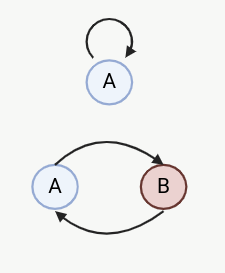
\includegraphics[width=7cm]{images/autocatalytic_motif.png}
    \caption[Autocatalytic motifs]{Autocatalytic motifs. Direct autocatalyis (top) and indirect autocatalysis (bottom).}
    \label{fig:autocatalysis_motif}
\end{figure}


Negative feedback can also be a means of destabilizing a system. A classic example is the repressilator,  a three gene loop where each gene expresses a protein that represses the next gene in the loop (figure \ref{fig:repressilator}) \cite{Elowitz2000}. The repression of gene X causes expression of gene Y to increase. Gene Y represses gene Z, which eases the repression of gene X, etc. Time delay is achieved with the transcription and translation of the three genes. The invention of the repressilator was a landmark achievement in the field of synthetic biology showcasing the feasibility of engineering complex gene circuits with predefined functions. It provided a foundational framework for the design and construction of synthetic genetic oscillators and inspired subsequent research in the development of artificial gene regulatory networks.

\begin{figure}
    \centering
    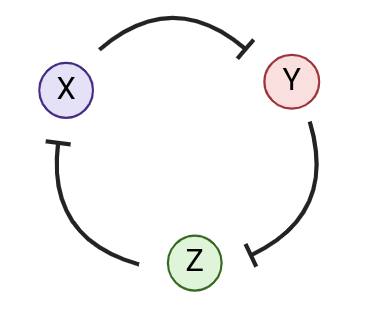
\includegraphics[width=7cm]{images/repressilator.png}
    \caption[Three node repressilator]{A three species repressilator.}
    \label{fig:repressilator}
\end{figure}

\subsection{Types of Oscillators}
The two primary means of destabilizing a system give rise to two basic types of oscillators: one based on negative feedback and one based on the combination of negative and positive feedback \cite{sauro_network_2009}. Both types of oscillators have been found in biological systems \cite{Tyson2003}.

\subsubsection{Negative Feedback Oscillators}
Negative feedback oscillators, such as the repressilator, require some sort of delay and the correct strength of feedback. The time delay allows the signal to go out of phase.
As the delay becomes longer, such as in systems with several intermediate steps, less feedback inhibition is needed to destabilize the system. Negative feedback oscillators tend to have smooth waveforms \cite{sauro_network_2009}.

The circadian clock is an example of a biological negative feedback oscillator (figure \ref{fig:circadian}). The proteins BMAL1 and CLOCK dimerize and activate the transcription of the proteins CRY and PER. These proteins accumulate in the cell, dimerize, and are transported back to the nucleus where they inhibit BMAL1/CLOCK induced transcription \cite{Rossetti2012}.

\begin{figure}
    \centering
    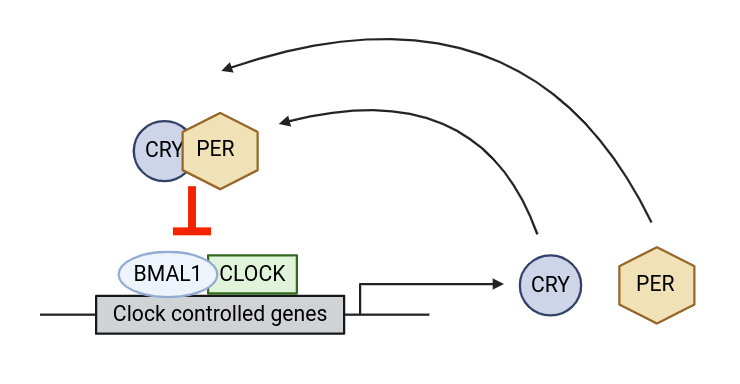
\includegraphics[width=12cm]{images/circadian.png}
    \caption[Negative feedback oscillation of the circadian cycle]{The circadian cycle is a negative feedback oscillator.}
    \label{fig:circadian}
\end{figure}

\subsubsection{Relaxation Oscillators}
Relaxation oscillators contain a subsystem that can be bistable, meaning it has two equally likely but different stable states. Bistability occurs over a range of values of a suitable control parameters, meaning there are limited values for the system to exist in either state. When the parameter moves beyond the range of values, it moves to the other steady state \cite{Sharma2006}.

For example, a bistable system with chemicals x and y is shown in figure \ref{fig:bistability}. The overlapping lower and upper curves represent the two stable states of the system. Moving along the lower curve, there is a point at which the lower steady state no longer exists for those values of x. At this point the system transitions to the upper steady state. Similarly, moving along the upper steady state, the concentration of x eventually exits the range of values for with the upper steady state exists and transitions back to the lower steady state.

A relaxation oscillator works by charging a species, in this example x, until it reaches a threshold with changes the state of the system. Once the system returns to its original state, the sequence begins again \cite{sauro_network_2009}. The charging and rapid switching of the relaxation oscillator leads to much sharper oscillations.

\begin{figure}
    \centering
    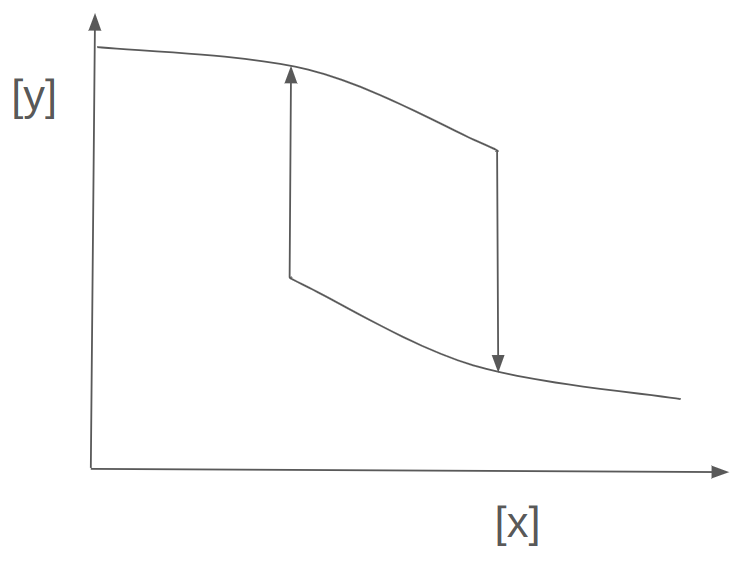
\includegraphics[width=12cm]{images/bistability.png}
    \caption[A simple bistable system]{A simple, two species, bistable system.}
    \label{fig:bistability}
\end{figure}

A biological example of a relaxation is the pacemaker action potential in the sinoatrial (SA) node of the heart \cite{SAnode}. The pacemaker cells in the SA node slowly depolarize as positive ions pass into the cell. When the cell's potential reaches a threshold value, calcium channels open causing an influx of calcium and rapid depolarization until the cell has a positive voltage relative to its environment. This voltage triggers potassium channels which pump potassium out of the cell and return it to its negative voltage where the cycle is repeated.

\subsection{Biological Relevance}
A fundamental aspect of living systems, oscillators occur across several levels of biological organization. 

As mentioned previously, the circadian clock exemplifies a well-studied molecular oscillator that regulates daily rhythms in behavior, metabolism, and physiology across organisms \cite{circadianReview, circadianOverview}. At its core, the circadian clock consists of interconnected transcriptional-translational feedback loops involving clock genes and proteins. These feedback loops take the form of interconnected repressilators \cite{YAMASHINO2013, Pett2016}. These molecular oscillators synchronize cellular processes with the day-night cycle, optimizing organismal fitness and survival. Disruptions to circadian rhythms have profound implications for health, contributing to various disorders such as sleep disorders, metabolic syndrome, and mood disorders \cite{circadianReview}.


Beyond the circadian clock, molecular oscillators operate within cells to regulate diverse processes such as gene expression, signal transduction, and metabolic pathways. Examples include calcium oscillations \cite{Smedler2014}, cyclic AMP (cAMP) signaling \cite{Dyachok2006}, and oscillatory patterns of gene expression driven by transcriptional regulatory networks \cite{Cerone2012}. These intracellular oscillatory systems enable cells to respond dynamically to external stimuli, coordinate complex physiological responses, and maintain cellular homeostasis under changing conditions \cite{Cheong2010, Jolma2010}. Oscillations are also present in systems such as neuronal networks \cite{Cebolla2019}, cardiac muscle cells \cite{Weiss2010, Montano2001}, pancreatic beta cells \cite{Watts2014}, and glycolysis \cite{Ghosh1964}, among others, highlighting the importance of molecular oscillators in physiological function.

Synthetic oscillatory systems offer considerable potential for advancing biomedicine and biotechnology. These dynamic systems can serve as biosensors, detecting the presence and concentration of proteins, drugs, and other chemicals \cite{Kis2015, CubillosRuiz2021}. Synthetic genetic oscillators can be employed to modulate the local delivery of effector molecules to tumors \cite{CubillosRuiz2021}. More broadly, synthetic oscillators could serve as essential components for engineering complex synthetic gene and protein networks. These networks could be used for disease diagnosis, pharmaceutical screening, and bio-manufacturing or used therapeutically to modulate endogenous oscillating systems \cite{Kis2015}.




\section{Applications of Evolutionary Algorithms in Systems Biology}
\label{section:intro_GA}
Genetic and evolutionary algorithms are optimization techniques inspired by the principles of natural selection and genetics. These algorithms mimic the process of natural evolution to solve complex optimization problems across various domains. At the core of genetic algorithms lies the concept of natural selection, a fundamental mechanism driving evolution in biological systems. Natural selection operates on populations of individuals, favoring those with traits that confer a reproductive advantage. Over successive generations, beneficial traits become more prevalent in the population, leading to the emergence of better-adapted individuals.






Evolutionary algorithms offer a computational framework for addressing the inherent complexity and nonlinearity of biological systems, providing a means to explore large solution spaces and optimize model parameters and structures.



The use of evolutionary algorithms in systems biology became popular in the late 1990s, often to better understand metabolic pathways. This approach has been used to demonstrate the optimality of the glycolysis \cite{Heinrich1999, stephani1999} and the Krebs citric acid cycle \cite{mittenthal2000}. In these studies, genetic algorithms were used to optimize reaction rates but not the structure of the networks.

Francois and Hakim evolved both the structure and reaction rates of genetic regulatory networks in an effort to generate small genetic networks that functioned as bistable switches and oscillators \cite{francois_hakim_2004}. The  algorithm used only mutation and selection, avoiding crossover, to minimize the difference between the candidate networks' output and idealized time series data displaying the desired behavior. Francois and Hakim argued that one of their evolved oscillators was structurally similar to the networks responsible for the circadian rhythm. However, Chu extended this work and found no consistent patterns in the evolved oscillators \cite{Chu_oscillator}. She noted that it is computationally unfeasible to thoroughly examine all resulting networks, but argued that the similarity to the circadian rhythm was likely coincidental. Despite Chu's study occurring almost 20 years ago, the problem of thoroughly pattern mining evolved networks remains and issue. The results of these works encouraged the exploration of evolutionary techniques on similar problems.

Fujimoto et al. employed a similar strategy to study genetic networks leading to striped patterning and ultimately body segmentation in arthropods \cite{fujimoto_network_2008}. When analyzing the resulting networks, they found three distinct classes, feed-forward loops, feed-back loops, and interconnections between the two. These three classes reproduced various segmentation strategies observed in arthropods.

Kobayashi et al. also explored the evolution of oscillatory genetic networks, however their algorithm fixed parameter values and only allowed connection rewiring to achieve oscillations with prescribed time periods \cite{kobayashi_evolutionary_2010}. Deckard and Sauro expanded this concept beyond genetic regulatory networks to evolve small networks with specific computational capabilities such as square root and cube root calculators \cite{deckard_preliminary_2004}. As with the previously mentioned algorithms, their algorithm avoided crossover relying solely on mutation to develop candidate solutions. Attempts to use crossover did not result in fitter offspring, possibly due to combining heterologous networks and thus disrupting developing solutions. This work was continued by Paladugu et al., who sought to generate mass-action network functional modules with specific behaviors, including oscillators \cite{Paladugu2006}.  This algorithm avoided crossover as the authors argued that it would be disruptive.

Marchisio and Stelling argued that brute force optimization algorithms lack efficiency and that implementing some element of rational design could speed up automatic design of genetic networks implementing boolean logic gates \cite{marchisio_automatic_2011}. They separate structural and parameter optimization by first generating several possible circuits and then ranks feasibility based on the structure. Then the best solutions undergo parameter optimization. Separating structural design from parameter optimization certainly saves computation time, but it relies on the existence of a rational solution, and is better suited for genetic networks, where these attributes are more easily separated. For more complex tasks, a solution might depend on a precise combination of both structure and parameter.

Other approaches fix structure and make use of evolutionary algorithms to explore the parameter space while fixing network topology. Jin and Sendhoff used an evolution strategy to explore parameters of regulatory motifs with fixed structures \cite{jin_evolving_2008}. Porubsky and Sauro use an evolutionary algorithm to search for parameters that yield oscillations in mass-action networks of fixed structure \cite{porubsky2019}.

Most applications of evolutionary algorithms in systems biology avoid the use of crossover as it tends to disrupt candidate solutions. For example, Drennan and Beer successfully evolved a repressilator using a genetic algorithm that included crossover \cite{drennan_beer}. Instead of evolving sets of differential equations, Drennan and Beer encoded their genetic regulatory networks using strings of 4 different letters, analogous to DNA encoding. Knabe et al. used a similar approach to evolve oscillators that interact with the environment \cite{knabe}. This approach allows for the straightforward implementation of crossover, but limits the space of possible models. Due to this encoding, there was a high probability of breaking connections making it difficult to pass on structural innovations.

Stanley and Miikkulainen addressed this problem in 2002 with NEAT (NeuroEvolution of Augmenting Topologies), a powerful algorithm used for evolving artificial neural networks (ANNs) \cite{stanley_evolving_2002}. Unlike traditional methods of neural network training, which typically involve adjusting the weights and biases of fixed network architectures, NEAT evolves both the structure and weights of neural networks simultaneously. Two key features of NEAT are the use of a more meaningful structural crossover technique, and speciation, which protects innovations and allows them time to develop by having candidate solutions compete only against similar individuals instead of the entire population. Dinh et al. adapted this technique to genetic regulatory networks and found improved performance in evolving oscillators with the use of crossover \cite{dinh_effective_2015}.

\section{Tools for Evolutionary and Genetic Algorithms}
\label{section:tools_GA}
Although there are many tools that enable evolutionary algorithms and simulating chemical reaction networks, there are none that facilitate evolutionary algorithms using chemical reaction networks. The two main issues with packages described here are user-friendliness and network encoding.

All of the tools described here require at least basic programming knowledge. Some packages boast extreme customizability, but require the user to essentially use the package as building blocks to write their own evolutionary algorithm program. These tools have significant barriers for users whose focus is not software development and programming.

Perhaps the larger issue is that all packages described here are intended for ``classic" evolutionary algorithm applications, where solutions can be encoded as vectors or matrices of integers and floating point numbers. This is not the case for the problem of evolving reaction networks, where candidate solutions are entire networks. To completely describe a chemical reaction network, an encoding must include (at the minimum) numerous reactions, including reactants, products, and rate constants and initial concentrations for each chemical species.  

\subsection{Python Libraries}

Most packages for implementing genetic and evolutionary algorithms are written in python \cite{python3}. Python is one of the most ubiquitous programming languages frequently topping lists of the most commonly used languages. It is often used in scientific applications due to it being open source, easy to use, and having vast library support. Likely for these reasons, most existing evolutionary algorithm tools are python libraries.

Although likely not an exhaustive list, the main python packages for evolutionary and genetic algorithms are described here.


\subsubsection{DEAP}
In 2012, Fortin et al. released the python package DEAP (Distributed Evolutionary Algorithms in Python) \cite{DEAP_JMLR2012}. The packages offers a toolbox of evolutionary algorithm features including different types of crossover, evolutionary strategies, and mutation operators. Unlike other frameworks DEAP makes algorithms explicit and data structures transparent, as opposed to black-box frameworks. Although DEAP allows for extensive customization, individuals are represented as arrays of values. Users can customize these arrays, such as specifying integers or floats at specific locations, but individuals must be in this form. For most optimization problems, this representation is adequate, however it is difficult to fully represent a chemical reaction network in this form. Reaction networks have varying numbers of reaction, so a stoichiometry matrix would be inadequate unless it contained a row for every possible reaction. Additionally, reactions require rate constants, and networks require initial values for each species. 

But beyond the encoding issue, the DEAP package, while highly versatile and proven in many research application, requires extensive programming knowledge. For example to build a population, a user must: (1) register the data type for each gene, (2) register an individual that combines these gene data types, (3) register a population that uses the individual, and finally (4) build the population. Running an entire genetic algorithm requires far more additional programming. 

\subsubsection{Pyevolve}
Pyevolve is a simpler framework for genetic algorithms compared to DEAP but has limited features \cite{pyevolve}. Despite its relative simplicity, it still requires extensive programming knowledge to implement an evolutionary process and problems are still limited to those whose ``genes" can be encoded as arrays of numbers. 

Pyevolve also requires significantly more programming to accomplish the same task comapred to DEAP. DEAP requires 59 lines of code to solve the OneMax problem\footnote{The OneMax problem is a classic problem in the field of evolutionary computation. It is a simple bit sting problem where the objective is the maximize the number of ones in a binary string. The fitness of each individual is the total number of ones in its string. The simplicity of the OneMax problem makes it an ideal benchmark for testing optimization algorithms}, compared to 378 for pyevolve \cite{LEAP}. 

The most recent release was 2014 and the library is no longer maintained.

\subsubsection{EasyGA}
EasyGA is a more recent (2021) python tool for genetic algorithms \cite{easyGA}. EasyGA makes it relatively easy to implement simple genetic algorithms, but still requires the user to have some advanced programming knowledge. The simplicity of easyGA makes it useful to only selected problems due to gene encoding restrictions.

The library has a limited number of genetic operators. Additionally, EasyGA randomly mutates both parents and offspring, a feature that goes against the basic premise of genetic algorithms. 

\subsubsection{LEAP}
LEAP (Library for Evolutionary Algorithms in Python) is another recently developed library published in 2020 \cite{LEAP}. LEAP was designed to simplify the process of implementing evolutionary and genetic algorithms. However, LEAP has some core design weaknesses that impact usability. 

Despite one of the objectives of LEAP being to simplify the process of implementing genetic algorithms, it still requires the user to write the evolution loop resulting in more code to solve simple problems. The user also has to manually increment the generation counter by calling a function specific to this purpose. Failing to call the function results in an infinite evolution loop, a problem that may not be immediately identifiable and solvable by less experienced users.

Additionally, LEAP has no means of tracing the results of each generation of evolution. This makes troubleshooting more difficult and renders LEAP an ineffective tool for those who may wish to study the evolution process and not just the final results.


\subsubsection{PyGAD}
In 2020, pyGAD was released with the aim to simplify the implementation of genetic algorithms for users with less programming experience while simultaneously proving control over ``everything possible" \cite{gad2023pygad}. PyGAD requires 3 core steps: (1) build the fitness function, (2) instantiate the relevant genetic algorithm class, (3) call the run function. The operation of pyGAD is relatively simple. Some programming knowledge is required for the user to create a fitness function and implement any further customization, but the bulk of the algorithm is run automatically. 

As with the other software tools described here, the main drawback of pyGAD for applications in systems biology is the restrictions on encoding individual solutions. Solutions must be encoded as a 1D vector of numbers. This is insufficient for evolving chemical reaction networks, where a solution is an entire reaction network and all parameters needed to simulate the network.

\subsubsection{EvoX}
Most recently, Huange et al. released EvoX, a python library for evolutionary computing \cite{Huang2024}. Unlike other libraries described here, EvoX is optimized for distributed GPU acceleration. This improves scalability and performance while remaining in the Python ecosystem.

\subsection{Libraries in Other Languages}
Python is one of the more commonly used languages for scientific computing, however other languages offer various advantages. C++ and Java offer high performance compared to interpreted languages, but tend to have steeper learning curves and are less common in scientific computing. R excels at statistical computing but is less versatile than python. MATLAB is proprietary and has high licensing costs. Julia is a relatively new language (2012) and has less package support and a smaller community than python. Likely for these reasons, fewer evolutionary packages exist in other programming languages and are less likely to be used by scientists. Notable non-python packages are briefly reviewed here.

\subsubsection{Evolutionary Computation in Java}
Evolutionary Computation in Java (ECJ) is a framework that supports several evolutionary computation techniques including genetic algorithms and differential evolution \cite{Luke1998ECJSoftware}. It offers a high level of flexibility and customization and is well-suited for large-scale optimization problems. 
ECJ has a steeper learning curve compared to other frameworks, especially for those not familiar with Java programming. Java is less frequently used in scientific programming making ECJ beyond the reach of many computational biologists. 

\subsubsection{JMetal}
Jmetal is a well-documented Java library offering a range of evolutionary algorithms and metahueristics for multi-objective programming \cite{Durillo2011}. It provides good performance and scalability for large-scale optimization problems. However, it requires knowledge of Java programming and a deeper understanding of the framework in order to customize it beyond the built-in algorithms. 

\subsubsection{Bio-Inspired Algorithms Building Blocks}
Bio-Inspired Algorithms Building Blocks (openBEAGLE) is a library providing evolutionary computation tools and components \cite{Gagne2006}. Written in C++, it offers good performance for  intensive tasks. However, it's documentation and community support are limited compared to more widely used frameworks and it may have a steep learning curve for those not familiar with C++.

\subsubsection{Many-Objective Genetic Metric-based Algorithms}
Many-Objective Genetic Metric-based Algorithms (MAGMA) is a library for many-objective optimization problems with a range of performance metrics for evaluating algorithms \cite{Wang2023}. It is written in MATLAB making it more accessible to many scientific users, however this limits performance for large-scale optimization problems compared to compiled languages.

\subsubsection{Genetic and Evolutionary Algorithm Toolbox for use with MATLAB}
Genetic and Evolutionary Algorithm Toolbox for use with MATLAB (GEATbx) seamlessly integrates with MATLAB's core functionalities, making it easy to implement and test evolutionary algorithms within the MATLAB environment \cite{pohlheim1994geatbx}. MATLAB's rich visualization capabilities allow users to easily visualize optimization processes and analyze results, aiding in understanding and debugging algorithms. GEATbx can be easily integrated with other MATLAB toolboxes for tasks such as data preprocessing, feature selection, and model evaluation, facilitating end-to-end optimization workflows. While MATLAB provides a wide range of functions for implementing evolutionary algorithms, the level of customization may be limited compared to lower-level languages or more specialized frameworks, particularly for advanced users requiring highly customized algorithms or optimization processes.
 
 
\subsubsection{Genetic Algorithms}
Genetic Algorithms (GA) offers a simple and intuited interface for implementing genetic algorithms in R, making it accessible to users with varying levels of programming experience \cite{GA1, GA2}. It has a range of customization options, including different selection methods, crossover and mutation operators, and termination criteria, allowing users to tailor algorithms to their specific problem domains. GA supports parallel execution, enabling users to leverage multi-core processors for faster execution of genetic algorithms, particularly useful for computationally intensive tasks. The package is actively maintained and updated by the R community, ensuring compatibility with the latest versions of R and incorporating new features and improvements over time. While suitable for many applications, R may not offer the same level of performance as lower-level languages like C++ or Java, especially for large-scale optimization problems or computationally intensive tasks.

\subsubsection{GALGO}

Like the GA package, GALGO integrates seamlessly with the R programming language, allowing users to leverage the rich ecosystem of statistical and machine learning libraries available in R \cite{Trevino2006}. GALGO offers a variety of evolutionary algorithms beyond genetic algorithms, including differential evolution, particle swarm optimization, and simulated annealing, providing users with flexibility in choosing the most suitable algorithm for their optimization problem. The package allows users to customize various aspects of the evolutionary algorithms, such as population size, crossover and mutation operators, and termination criteria, enabling tailored solutions for different optimization tasks. Like GA, GALGO may suffer from performance limitations compared to compiled languages.

\subsubsection{Evolutionary.jl}
Evolutionary.jl offers a user-friendly interface for implementing evolutionary algorithms in Julia, making it accessible to users with varying levels of programming expertise \cite{evolutionary.jl}. The package provides a range of evolutionary algorithms, including genetic algorithms, differential evolution, and particle swarm optimization, among others, allowing users to choose the most suitable algorithm for their optimization problems. Evolutionary.jl allows users to customize various aspects of the evolutionary algorithms, such as population size, crossover and mutation operators, and termination criteria, enabling tailored solutions for different optimization tasks. Julia is designed for high-performance numerical computing, and Evolutionary.jl benefits from Julia's performance advantages, providing efficient execution of evolutionary algorithms. However, this package is not suited for evolving chemical reaction networks due to the limitations of encoding solutions.

\section{Julia Packages for Reaction Network Modeling}
\label{section:tools_networks}
There are two primary packages for simulating chemical reaction networks in the julia programming langauge: RoadRunner and Catalyst. Although both offer a range of functionality for network modeling, they were not suitable for use in a julia package for generating reaction networks using genetic algorithms. The problem with both packages is the manner in which reaction networks are encoded.

RoadRunner is one of the fastest network simulation tools and has an interface for both python and julia \cite{Welsh2022}. It achieves its performance advantage by compiling reaction network models directly into native machine code. For evolutionary algorithms, where a network must be frequently modified and re-simulated, the performance advantage is lost as the network must be repeatedly converted to machine code after each sight modification.

Catalyst is a julia package for analysis and high performance simulation of chemical reaction networks \cite{Loman2023}. Catalyst converts chemical reaction networks to symbolic representations of concrete mathematical models and generating compiled code for numerical solvers. It includes several tools for analyzing, visualizing, and simulating networks making it highly versatile and relatively user friendly. However, Catalyst's reaction network object makes it difficult to modify the topology of reaction networks automatically making it unsuitable for genetic algorithms. 

\section{Conclusion}
Due to their interesting dynamics and biological relevance, chemical oscillator research has blossomed over the past 100 years. Their varied topology and interesting dynamics makes oscillation a compelling problem to explore with evolutionary algorithms. However, although evolutionary algorithms have been used to study and generate oscillators and other network behaviors, the software used for these studies was designed for one-time use and was not made available to the public. Additionally, previous research suggests that simple evolutionary algorithms have low success rates in generating oscillators.

There are numerous software tools for evolutionary algorithms and simulating chemical reaction networks, but none of these existing tools are suitable for using evolutionary algorithms on chemical reaction networks. Despite the interest in such a tool, as demonstrated in previous studies, there is no software tool that enables the evolution of chemical reaction networks in a speedy, user-friendly manner with a decent success rate.

\chapter{A Public Database of Evolved Oscillatory Reaction Networks}
\label{chap: cesium_paper}
\section{Background}
\blfootnote{This chapter was published in as
Tatka, L., Luk, W., Hellerstein, Elston, T., J., Sauro, H. “Cesium: A Public Database of Evolved Oscillatory Reaction Networks.”  Biosystems, vol. 224, 2023, p.104836., \\
https://doi.org/10.1016/j.biosystems.2023.104836. } With the constant emergence of new software tools and techniques in systems biology, access to a large variety of chemical reaction network models with defined characteristics can be useful for testing and validation. For example, an existing data set enumerating small chemical reaction networks~\cite{deckard2009} has been used to test computational methods to analyze bistability~\cite{pantea2010}, software to reverse engineer networks~\cite{nobile2013}, and a novel framework to assess networks for multiple equilibria and other characteristics~\cite{donnell2014}. Generating these test data sets can be computationally expensive and time-consuming. The data set generated by Deckard et al. took several days to compute and contains approximately 47 million small models, but its purpose is to exhaustively enumerate small networks, not to assess and catalog their behavior~\cite{deckard2009}.  Despite the usefulness of standard validation data sets, currently no public database exists containing numerous models displaying a variety of network behaviors.

In terms of network behavior, oscillatory chemical reaction networks are of particular interest due to their biological relevance, including embryogensis, DNA repair, and heart function~\cite{Novak2008,Aulehla2008,GevaZatorsky2006, Pol1928}. Lotka et al. documented the first ordinary differential equation model of an oscillatory predator-prey network~\cite{Lotka1910}. The study of oscillatory mechanisms in chemical reaction networks dramatically increased with the expansion of computing power and the improved ability to solve non-linear differential equations~\cite{Higgins1967}. Novak and Tyson studied non-autocatalyic small oscillators to determine design patterns and basic requirements for oscillating systems~\cite{Novak2008}. These works focus on the mechanisms and characteristics of individual oscillators or to oscillators as a broad category. Paladugu et al. used in silico evolution to create several oscillators, bistable switches, homeostatic systems and frequency filters, but the library was not made publicly available for further study~\cite{Paladugu2006}. 

We present a public database, entitled ``Cesium",  containing approximately 1800 3-species, 450 6-species, and 750 10-species oscillating networks created using a customized evolution algorithm, an optimization process based on the iterative improvement of candidate models. There are also random non-oscillating networks to serve as controls. The database can be searched by the number of reactions, the presence of autocatalytic reactions, and the number of species. Each entry contains the above information as well as the Antimony string~\cite{Smith2009} of the model which can be simulated by any software capable of reading antimony or SBML (to which Antimony models can be converted). Future work will expand this database to include a wider variety of oscillatory models as well as models that display other behaviors such as bistability. 

The population of evolved oscillatory reaction networks possessed different reaction type compositions compared to non-oscillating networks that were randomly generated. Oscillating networks had significantly more uni-bi reactions and autocatalytic reactions. 


\section{Methods}
Oscillating models were generated using evolution scripts written in python, available at https://github.com/sys-bio/evolution. The process begins by randomly generating a population of models and gradually modifying them over time to produce oscillatory behavior. Four types of reactions are used: uni-uni, uni-bi, bi-uni, and bi-bi, all with mass-action kinetics (figure \ref{fig:reaction}). At each step, every model is evaluated against an objective function scoring the model's ability to oscillate. Models with better fits are selected and further modified and models with lower fits are gradually eliminated. 
% \begin{wrapfigure}{r}{0.5\linewidth}
% \centering
\begin{figure}
    \centering
    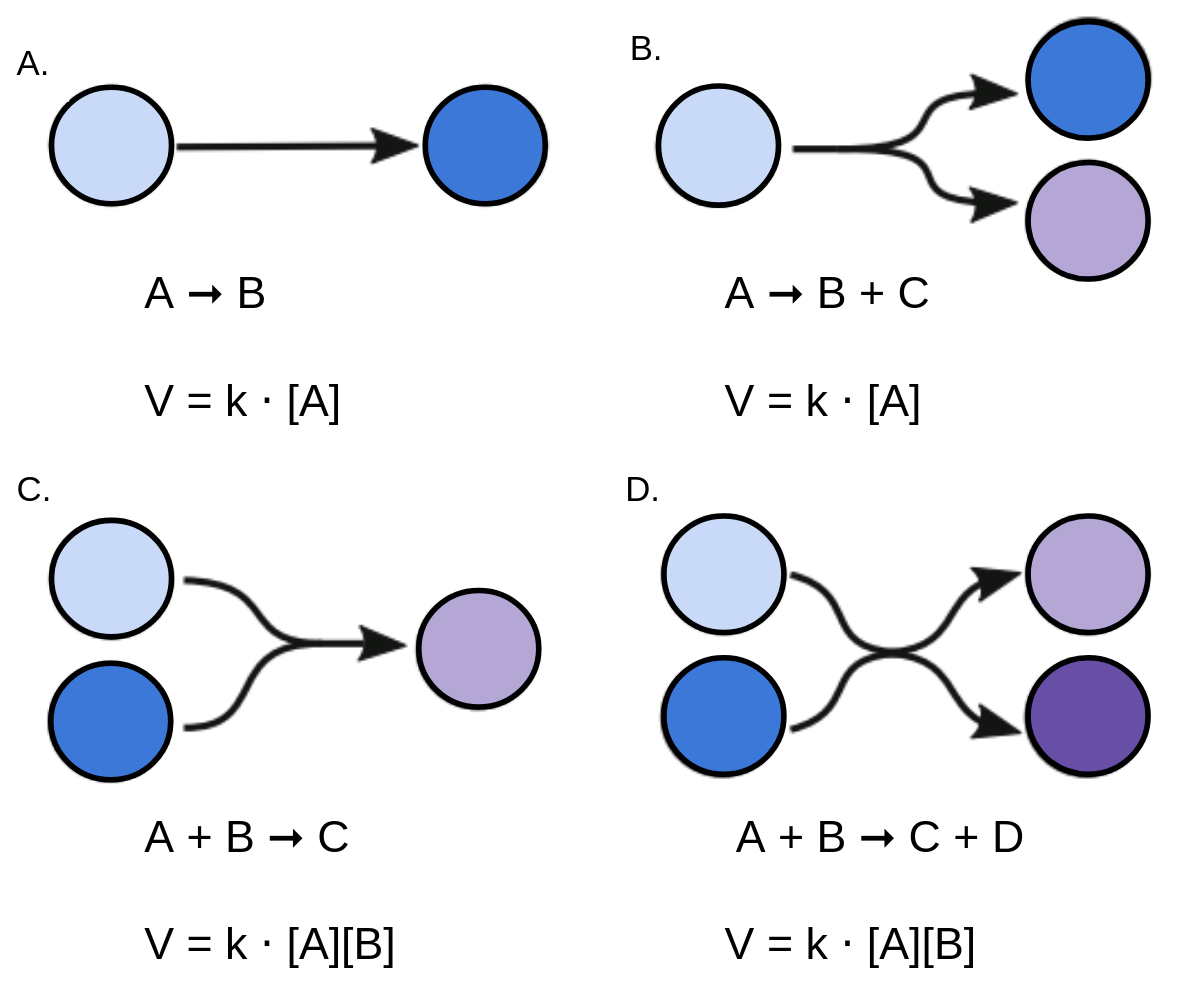
\includegraphics[width=10cm]{images/Reactions.png}
    \caption[Types of reactions and their rate laws]{Models were composed of four reaction types and rate laws: (A) uni-uni, (B) uni-bi, (C) bi-uni, (D) bi-bi}
    \label{fig:reaction}
    
\end{figure}



\subsection{Model Representation}
Models and reactions were represented by custom data structures. An instance of the \textit{reaction} object represents a single reaction and consists of one or two reactants, one or two products, a rate constant, and an integer representing the reaction type (uni-uni, uni-bi, bi-uni, or bi-bi). The \textit{model} object represents a single reaction network and consists of a list of species, a list of initial concentrations, and a list of \textit{reaction} objects. The software converts \textit{model} objects into systems of ordinary differential equations which are then numerically solved to produce time series data of species concentrations. After the evolution process is complete, the models are converted to antimony~\cite{Smith2009}, a human readable model definition language.

\subsection{Objective Function}

The objective function minimized error between the candidate model's time course data and a series of points corresponding to the peaks and troughs of an oscillator. This "idealized" oscillator time series consisted of nine concentration points, alternating between 5 and 30 concentration units over the course of 1.25 seconds (figure \ref{fig:fitness}). The output time series of each species was compared to these points by summing the squared difference between the observed point and the ``ideal" point and the smallest error value was considered the model's fitness. This is similar to MSE but the sum is not divided by the number of observations as this number is constant across all models. This has been demonstrated to be an effective objective function for the in silico evolution of chemical oscillators~\cite{Paladugu2006}.  In cases where candidate models could not be simulated, an arbitrarily high fitness value was assigned resulting in their subsequent removal from the population in the selection step.  

\begin{figure}
    \centering
    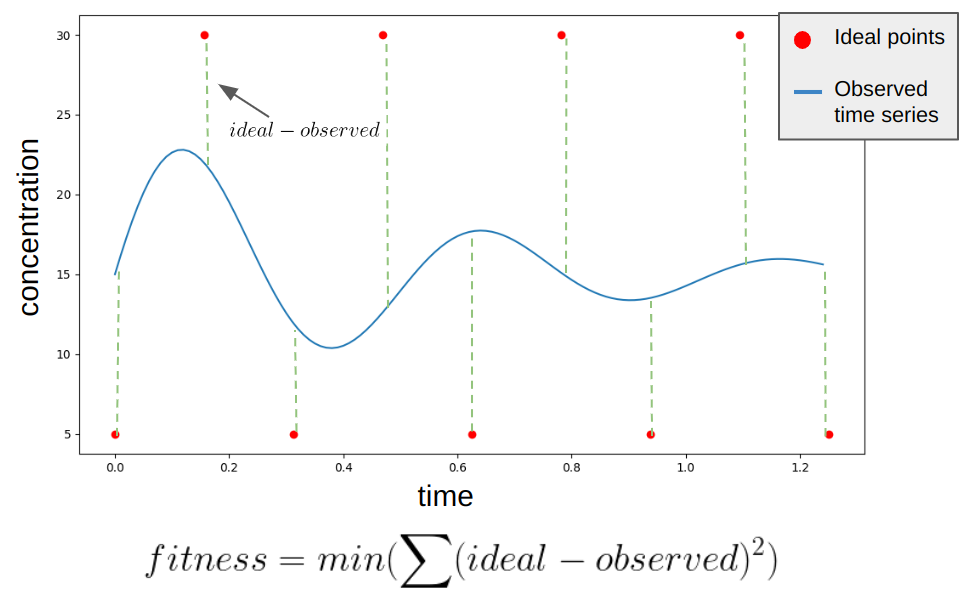
\includegraphics[width=15cm]{images/fitness.png}
    \caption[Oscillator objective function]{For the time series data of this species, the error is calculated by summing the square difference between the observed time series data (blue) and a set of idealized oscillator points (red). This process is repeated for each species in the model and the fitness is defined as the minimum of these sums. }
    \label{fig:fitness}
\end{figure}

\subsection{ODE Solver}
Preliminary studies suggested that the most commonly used python ODE solver from scikit was inaccurate for solving these problems. Other off-the-shelf solvers lacked the ability to deal with the custom data structure encoding the models. The Sauro Lab's simulation software, RoadRunner~\cite{Somogyi2015}, was also unsuitable for this purpose due to the computational cost of frequently modifying and recompiling models for simulation. Many algorithms, such as RK4 are not robust enough for this work. For this reason, a custom simulator using the CVODE solver from the Sundials suite was used~\cite{hindmarsh2005sundials}. 

\subsection{Selection}
In each new generation, the top 10\% of models from the previous generation were copied without modification. The remainder of the new population was chosen by tournament selection~\cite{Miller1995} from the previous generation. This is where two models are randomly chosen from the previous generation (including from the top 10\% of models already carried over) and the model with the better fitness is mutated by adding or deleting a reaction, or by modifying a rate constant. The modified model is then appended to the new generation. 

\subsection{Mutation}
After tournament selection, the fitter model was either mutated by modifying a rate constant or adding/deleting a reaction with equal probability. In the case of rate constant modification, a random rate constant was adjusted by a random percentage between -15\% and +15\% of the rate constant's current value. This mechanism ensured that rate constants could not become negative, and there was no upper limit to their value. 

In the case of reaction modification, a reaction was either added or deleted with 50\%-50\% probability. If deleted was selected, a random reaction was removed from the model. If addition, a new reaction was added with the equal probability of each reaction type: uni-uni, uni-bi, bi-uni, bi-bi (figure~\ref{fig:reaction}). 

\subsection{Random Networks for Evolution}
A population of 40 random networks were generated using the {\tt teUtils} python package~\cite{SauroteUtils_2020}. Each network was initialized with three species, and nine reactions with the probability of each reaction type being 0.1, 0.4, 0.4, 0.1 for uni-uni, uni-bi, bi-uni, and bi-bi reactions. These settings were chosen to maximize the number of evolution trials that successfully product oscillators. All reactions had mass-action kinetics with a random rate constant between 0 and 50. 
\begin{figure}
\begin{center}
    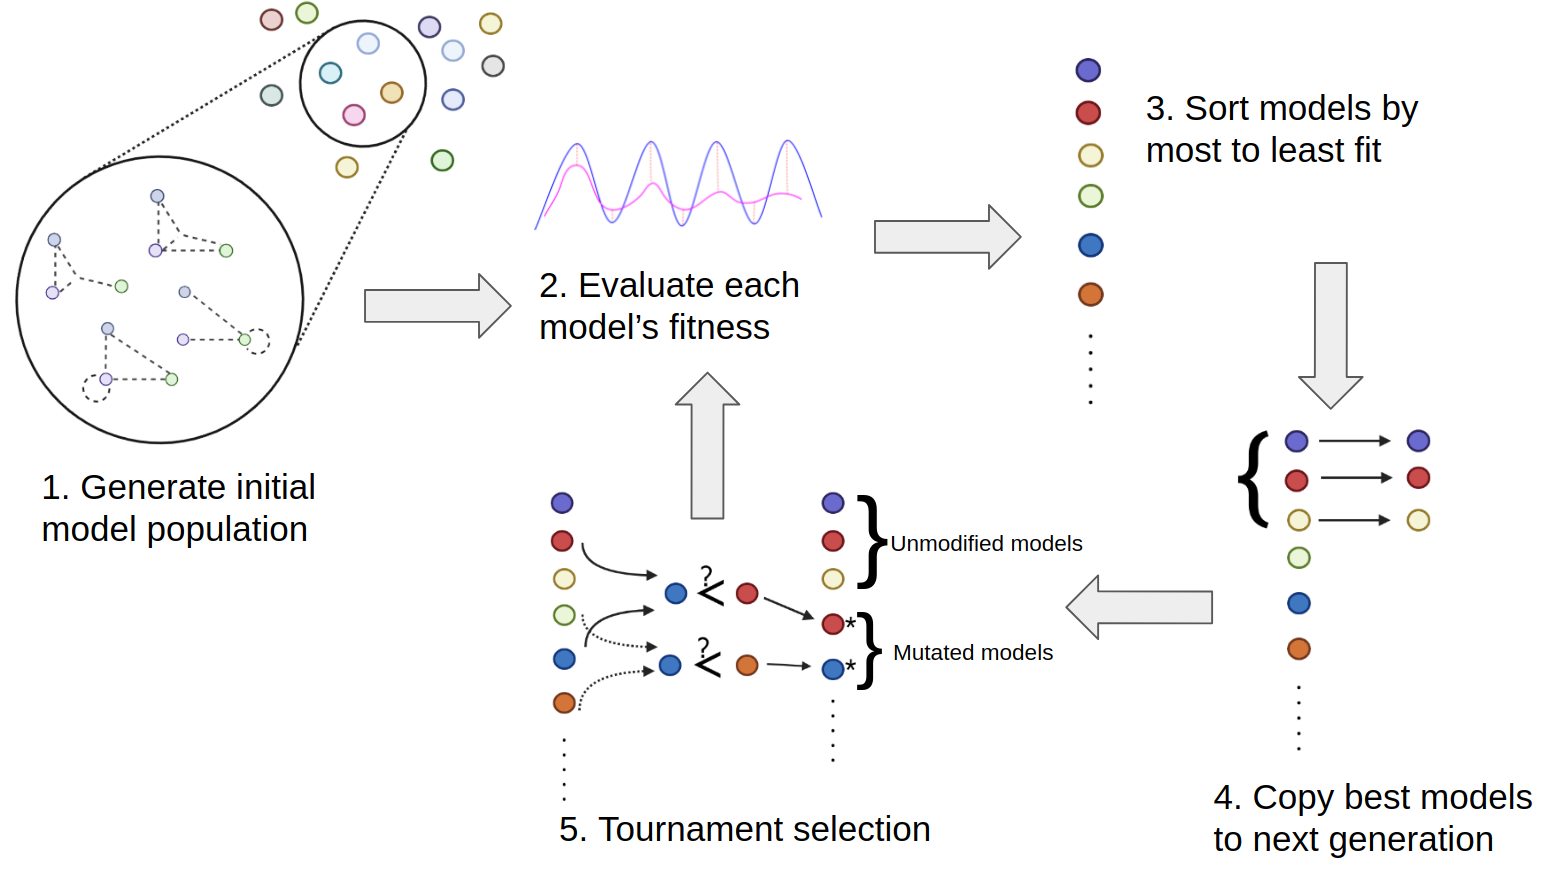
\includegraphics[width=17cm]{images/algorithm.png}
    \caption[Overview of the evolution algorithm in Python]{The evolution algorithm. (1) An initial population of random models is created. (2) The fitness of each model is evaluated. (3) The entire population is sorted by most fit to least fit. (4) The top 10\% of the models are transferred to the subsequent generation unmodified. (5)  Tournament selection is used to populate the remainder of the subsequent generation. Models are randomly selected, the more fit model is chosen to be modified and carried over to the subsequent generation. Steps 2-5 are repeated. }
    \label{fig:algorithm}
    \end{center}
\end{figure}

\subsection{Custom Evolution Algorithm}

The evolutionary algorithm mimics biological evolution in that populations of individuals, in this case candidate networks, are altered and forced to compete with each other. Over the course of generations, fitter individuals (models that oscillate or are likely to oscillate) out compete unfit individuals (models that do not oscillate or can not be simulated) and survive into the next generation. Although genetic and evolutionary algorithms are well characterized, their application to systems biology models remains a challenge as a key trait in these algorithms is crossover, the ability of two possible solutions to exchange information, creating a new, ideally more suitable, candidate solution~\cite{Katoch2020}. Typically, genetic algorithms operate on objective functions for which solutions consist of vectors where values can easily be exchanged between two vectors. It is uncertain how crossover of mass-action kinetic models could be achieved as solutions (candidate networks) consist both of topology (how reactions are connected) as well as rate constants (vectors of values). Additionally, the number of reactions and rate constants vary and must be equal but can vary from model to model. For this reason, a custom optimization process was developed based on genetic algorithms but avoiding crossover. 

This process begins with the generation of 40 random networks with pre-specified probabilities for each of the four reaction types.  The fitness of each model is evaluated by comparing the model's time series data with an objective function representing the desired outcome, oscillation. Models that with time series data close to this desired outcome, those that oscillate or those with damped oscillations, are more fit than those that fail to oscillate or cannot be simulated. 

These models are ordered from most to least fit and the top 10\% of the models are carried over unmodified to the subsequent generation (figure \ref{fig:algorithm}). The remaining models are randomly paired and compared and the fitter of the two models is slightly modified by either adding or deleting a reaction or changing a rate constant. If the modification improves the fitness of the model, the modified model is added to the next generation. If the modification makes the model less fit, 75\% of the time the unmodified model is added to the next generation and 25\% of the time the less fit model will be added. This allows for the chance that small changes initially make a model worse, but subsequent changes drastically improve the model. Once the new generation is fully populated, the models are again ordered from most to least fit and the process begins again. This is repeated for 400 generations or until a threshold fitness level is reached.

\subsection{Random Control Networks}
Random models were generated as described in the previous section. To control for changes made during evolution, the random models underwent the same mutation processes described previously. Instead of populating subsequent generations based on model fitness, 10\% of the previous population was randomly selected to be carried over unmodified to the new generation. The remainder of the new generation was populated with models randomly chosen and mutated from the previous generation. The purpose of this procedure was to account for model variability introduced in the evolutionary process. Of 1000 random control networks generated, 1 was a spontaneous oscillator.

\section{Results}
Evolved models are processed to remove any undesirable oscillators from the population, namely oscillators that dampen over time or oscillators where one or more species concentrations rise indefinitely towards infinity. Next,  duplicated reactions were fused and reactions that are superfluous to oscillation are deleted to minimize network size resulting in a population of reaction networks that oscillate indefinitely in species concentration, examples of which are shown in figure 4.

\begin{figure}
    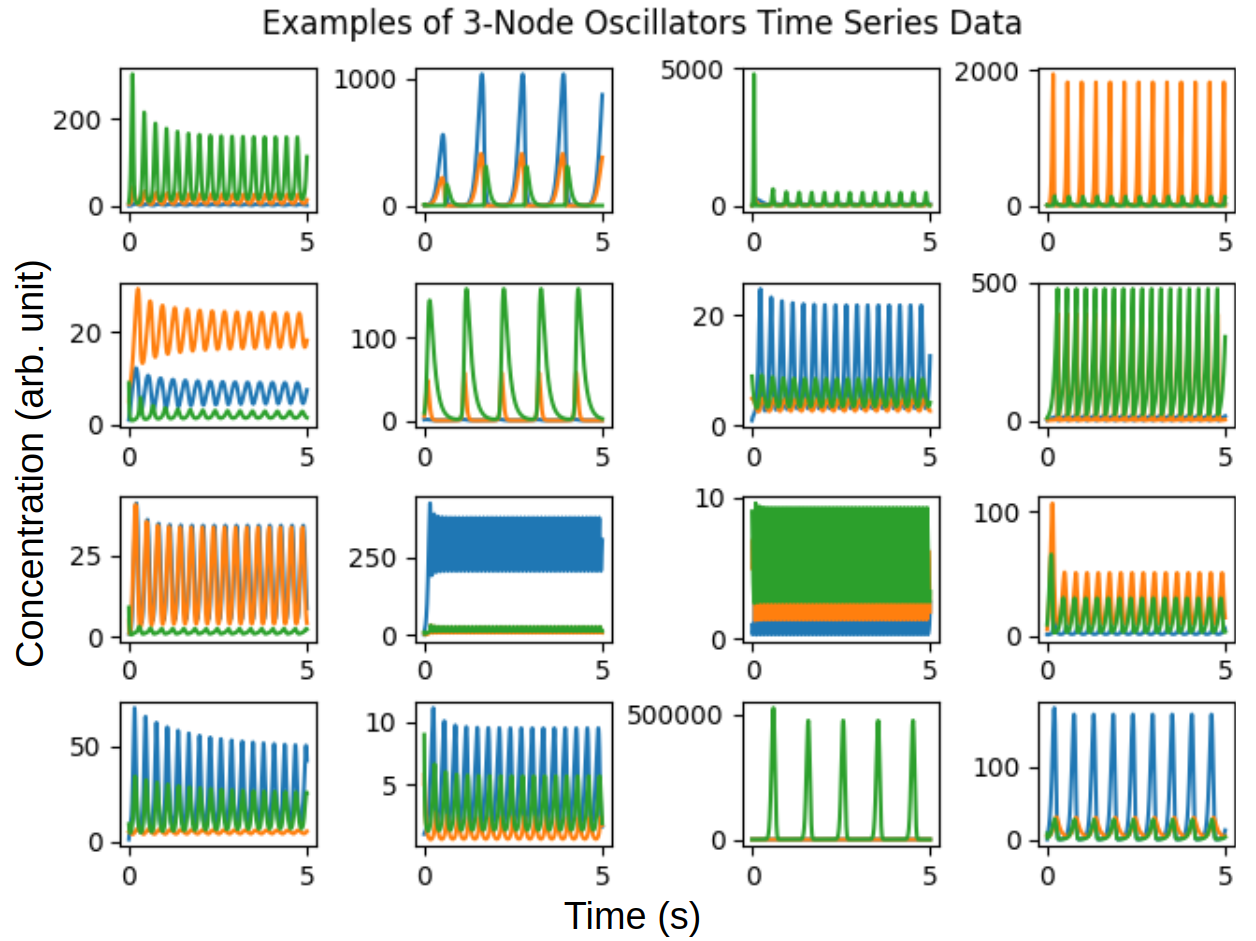
\includegraphics[width=15cm]{images/examples.png}
    \label{fig:examples}
    \caption[Examples of oscillator time series data]{Time series data of sixteen 3-node oscillators generated using differential evolution.}
\end{figure}


\subsection{Database Construction}
A non-relational key-value database was deployed via Mongo Atlas using the PyMongo API to store all models and their information. The user enters the desired reaction network attributes into the web GUI (figure \ref{fig:website}). Models are downloaded as a .zip file of text files, or if a single model a single text file, containing the antimony string of each model. If the ``Download in simulatable Tellurium form" box is checked, then each model file will contain the necessary python package imports and formatting to be immediately simulated and plotted upon running the file.


The current website queries the database by model type (current options are oscillator or random), the number of nodes (species), the number of reactions, and the presence or absence of autocatalysis or degradation reactions. Both oscillator and non-oscillating control networks are stored in the database. Each entry also includes a dictionary of tallies of each reaction type in the network, a list of redundant reactions that were fused during post-processing, a list of reactions that were deleted as their presence did not influence oscillation. 




In addition to the Antimony string comprising the model, other characteristics such as its initial reaction probabilities, fused and deleted reactions, and reaction counts are also tracked in the database.  The database can be queried to select models with any number of desired traits. Both oscillator and non-oscillating control networks are stored in the database.

The Cesium database is publicly available on the web at \url{https://cesiumdb.herokuapp.com/} and is intended to serve as source of reaction networks with specified characteristics for use in research and validation.  It currently contains 2000 randomly generated models and approximately 1800 3-species oscillating networks. This database can be expanded in the future to include a wider variety of oscillatory networks as well as networks with different behaviors, such as bistability. 

\begin{figure}
    \centering
    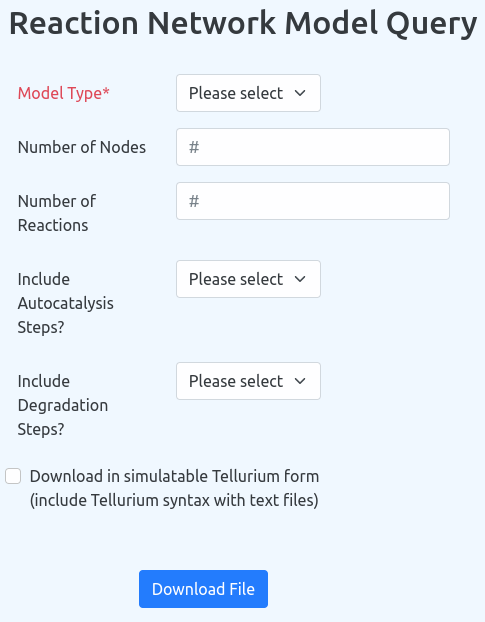
\includegraphics[width=12cm]{images/website.png}
    \caption[Landing page for the Cesium database website]{Landing page for the Cesium database.}
    \label{fig:website}
\end{figure}

\subsection{Oscillating Network Examples}
Four oscillating networks from the database are shown in figure \ref{fig:model-diagrams}. Arrows symbolize reaction and lead from the reactant to the product. A double headed arrow indicates two products are formed and a double tail indicates two reactants. 


\begin{figure}
    \centering
    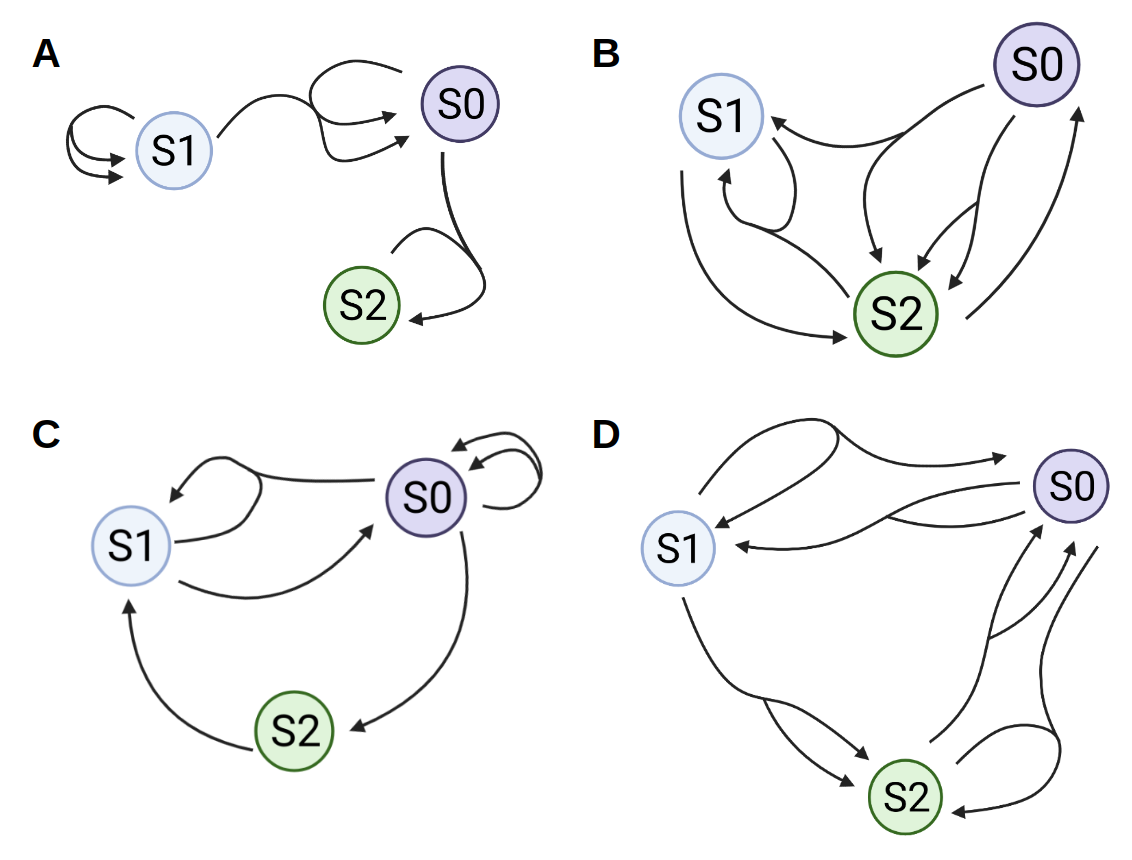
\includegraphics[width=12cm]{images/model-diagrams.png}
    \caption[Examples of evolved oscillating networks]{Examples of 3-species oscillating networks from the Cesium database.}
    \label{fig:model-diagrams}
\end{figure}

In network A, S1 is autocatalytic as is S0 (and catalyzed by S1). These linked positive feedback loops cause oscillation with products out flowing to S2, which essentially behaves as a boundary species, a species that is unaffected by the model and whose concentration remains fixed.  Network B lacks autocatalytic reactions completely. Computing the jacobian matrix at the unstable focus results in the following matrix:
\[
\begin{blockarray}{cccc}
S0 & S1 & S2 \\
\begin{block}{(ccc)c}
  -4.75 & 0 & 15.2 & S0 \\
  0.75 & -0.3 & 0 & S1 \\
  8.75 & -1.6 & -22.8 & S2 \\
\end{block}
\end{blockarray}
 \]
In the bottom row center, the negative number indicates that there is an inhibitory relationship between S1 and S2. An increase in S2 will decrease the production rate of S1. These interactions for a cycle with negative feedback, suggesting that this is a feedback oscillator (figure \ref{fig:feedback}). Similar analyses reveal that networks C and D are also likely to be feedback oscillators.

\begin{figure}
	\centering
    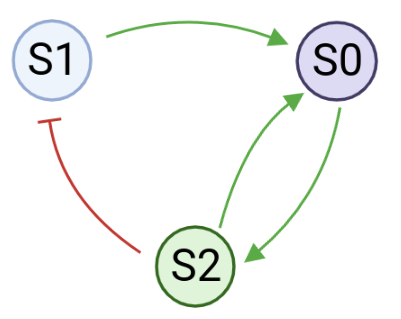
\includegraphics[width=8cm]{images/feedback-cycle.png}
    \caption[Feedback diagram of an oscillating network]{Species interactions of Network B. Green arrows indicate activation and blunt red arrows indicate inhibition. The interactions form a cycle with negative feedback suggesting that Network B is a feedback oscillator.}
    \label{fig:feedback}
\end{figure}


\section{Discussion}

Oscillating models were significantly enriched for autocatalytic reactions compared to control networks. Most oscillators are associated with unstable steady states. Destabilizing processes can be classified as 1) direct autocatalysis, 2) indirect autocatalysis (a positive feedback loop), and 3) end-product inhibition (a negative feedback loop)~\cite{Tyson1975, tyson2007}. Reactions are considered autocatalytic when the products increase the rate of reaction or when a chemical decelerates the rate of its own destruction~\cite{Tyson2004}. Given the two types of oscillators, negative feedback and negative feedback coupled with positive feedback~\cite{Sauro_dynamics}, it is unsurprising that autocatalytic reactions are enriched in the oscillator population as these reactions are a form of positive feedback. The portion of models containing at least one autocatalytic reaction in the oscillator and control populations were compared using a two-way chi square test. Of the 586 oscillating models, 83.1\% (487 of 586) contained an autocatalytic reaction compared with 49.8\% (498 of 1000) of the control models, a significant difference ($p < 0.0001$). 

Given the enrichment of autocatalytic reactions, one might expect a similar enrichment of degradation reactions, reactions where one species is removed from the system (eg. $X + Y \to Y$, where $X$ is removed from the system), to prevent species concentrations from rising to infinity. Interestingly, the presence of degradation reactions were not enriched in oscillating models. Of the oscillating model population 79.4\% (465 of 586) contained at least one degradation reaction compared to 76.3\% (763 of 1000) of the control models, an insignificant difference suggesting that although autocatalysis is a common characteristic in oscillating networks, degradation reactions are not necessary to prevent species concentrations from rising to infinity.  Although the presence of both an autocatalytic and a degradation reaction are not necessary for oscillation, it is rare that an oscillator contains neither. Only 0.5\% (3 of 586) of the oscillators analyzed had neither an autocatalytic reaction nor a degradation reaction compared to 0.2\% (2 of 1000) random models, an insignificant difference.

To determine if any reaction types were enriched in the oscillator population compared to the control population, the average model compositions were compared. The average model composition was assessed as the average number of reactions of the specific type were divided by the average total number of reactions for each group. For example, there were an average of 6.592 reactions per model in the oscillator population, of which an average of 0.99 were uni-uni reactions, for an average of 15.3\% uni-uni reactions in the average oscillator model (Table \ref{fig:avg-comp}). Compositions were compared with permutation tests, showing that model compositions and sizes were significantly different between the oscillator and control populations (the reduced size of oscillating networks can be accounted for by the fusion of duplicate reactions). Oscillators possessed significantly more uni-bi reactions compared to random control models. This is consistent with the enrichment of autocatalytic reactions which are often uni-bi. However, autocatalytic reactions can also be bi-bi reactions, which were not enriched in oscillating models. Although bi-bi reactions were less likely to be created during evolution due to the initial settings (10\%), it is somewhat surprising that bi-bi reactions were decreased in oscillatory networks given that a bi-bi reaction is slightly more likely to be autocatalytic ($\frac{4}{27}$) compared to a uni-bi reaction ($\frac{1}{9}$).

\begin{table}
	\centering
    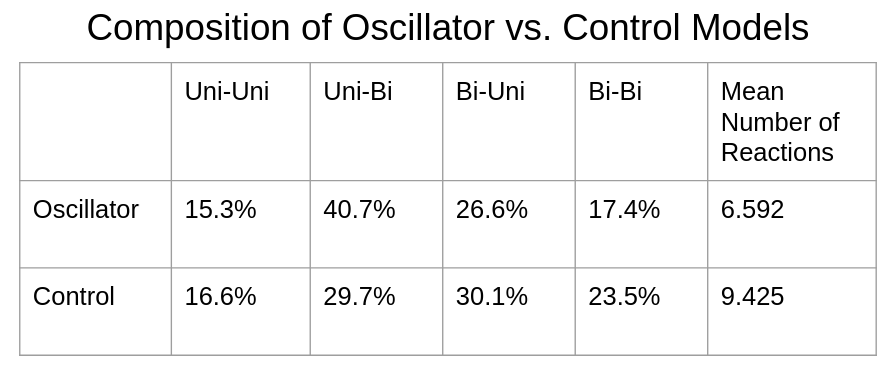
\includegraphics[width=12cm]{images/composition.png}
    \caption[Composition of oscillator vs. control models]{Average reaction compositions of oscillating networks compared to non-oscillating controls.}
    \label{fig:avg-comp}
\end{table}

Next, oscillators containing autocatalytic reactions (498 models) were compared to oscillators lacking them (98 models). Populations were compared by permutation test. There was a significant increase in the portion of uni-bi reactions and a significant decrease in the portion of bi-uni reactions in non-autocatalytic models as compared to autocatalytic oscillators (Table \ref{fig:autocatal}). This result is interesting given that autocatalytic reactions are either uni-bi or bi-bi and both reaction types were reduced in oscillators with autocatalytic reactions compared to oscillators without. It is possible that oscillators without a single autocatalytic reaction are achieving autocatalysis through a combination of non-autocatalytic reactions.

\begin{table}
	\centering
    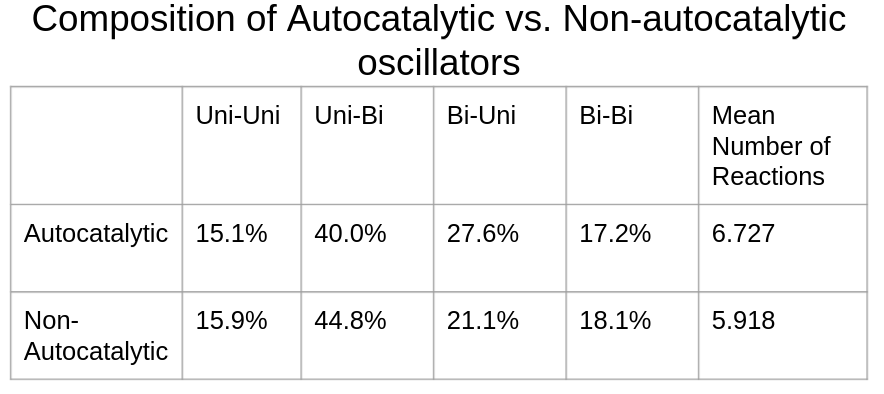
\includegraphics[width=12cm]{images/autocomp.png}
    \caption[Composition of autocatalyitic vs. non autocatalytic oscillators]{Average reaction compositions of autocatalytic oscillating networks compared to non-autocatalytic oscillating networks.}
    \label{fig:autocatal}
\end{table}

Several manually inspected oscillators had reactions with extremely high rate constants (greater than 300, whereas most rate constants were between 5 and 75). The initial range for rate constants is 0 to 50 and with each mutation, they can only increase a maximum of 15\% of the current value. Although there is no upper limit for rate constants, it is nearly impossible to mutate a rate constant from the initial range to over 100 during the course of evolution. To bypass this limit and achieve high rate constants, many successful models have simply duplicated reactions during the evolutionary process. During post-processing, these duplicate reactions are fused and their rate constants summed. Fusing duplicate reactions to achieve high rate constants accounts for the observation that oscillators generally have fewer reactions than non-oscillators in this study. These high rate constant reactions can not be removed, nor can the rate constant be significantly lowered without impacting oscillation. Further investigation is needed to determine what essential function these high rate reactions seem to play in most of the oscillators included in this study. 


These oscillatory models and the random control networks have been added to a database, accessible at \url{https://cesiumdb.herokuapp.com/}. Models can easily be selected by the number of species, the number of reactions, and the present of autocatalysis or degradation reactions. The selected models can be downloaded in a zip file containing a .txt for each model. Each .txt file contains an individual model's antimony string. If the ``Download in simulatable Tellurium form" option is selected, the .txt file will also contain formatting and package imports allowing the model to be easily simulated when the file is run as a python script. 

In the future, this database will be expanded to contain a variety of models with different behaviors besides oscillation. It is our hope that this database serves as a resource for the modeling community to study network behaviors and test novel software.


\section*{Funding}
This project was supported by National Institute of Health grant U01 CA238475 and the National Institute of Biomedical Imaging and Bioengineering for grant P41GM109824.

\section*{Acknowledgements}
We thank Lucian Smith for valuable discussions on differential evolution and model topology. 
\\



\chapter{In Silico Speciated Evolution of Oscillatory Mass-Action Reaction Networks}
\label{chap: ReactionNetworkEvolution.jl}
\section{Introduction}
Genetic algorithms (GAs), inspired by the principles of natural selection and genetics, have emerged as a powerful computational technique for solving optimization and search problems.Developed by John Holland in the 1970s, GAs mimic the process of biological evolution to solve optimization and search problems \cite{holland_1975}. At their core, genetic algorithms operate on a population of potential solutions, represented as individuals or ``chromosomes," each encoding a candidate solution to the problem at hand. Through iterative generations, genetic algorithms apply mechanisms of selection, crossover, and mutation to evolve and refine the population, gradually converging towards optimal or near-optimal solutions. Selection favors individuals with higher fitness, mirroring the process of natural selection, while crossover and mutation introduce variation and diversity into the population, allowing for exploration of the solution space. By leveraging the principles of evolution, genetic algorithms offer a versatile and robust approach to solving complex problems across various domains, from engineering and optimization to biology and beyond.

A key feature of genetic algorithms is crossover, the exchange of multiple parameters between two candidate solutions to create a new offspring solution. Crossover proves challenging when solutions are not vectors of matrices of numbers, but also include graphs. Stanley and  Miikkulainen devised a method, NEAT, to crossover topologies when evolving artificial neural networks \cite{stanley_evolving_2002}. Dinh et al. adapted NEAT to enable crossover when evolving gene regulatory networks \cite{dinh_effective_2015}. Here, the NEAT algorithm is adapted and explored with mass-action chemical reaction networks. In contrast to previous studies in different domains, the crossover method presented here does slightly reduces the success rate of evolution. 

Speciation, though not essential to evolutionary algorithms, can improve their success by protecting innovations and allowing them time to develop into better solutions. This work also introduces a method for separating chemical reaction networks into species and explores the effect of speciation on evolutionary success.

The purpose of this work it twofold: (1) to create a general purpose, easily customizable, module for evolving mass-action chemical reaction networks and (2) to explore the effects of crossover, speciation, and other hyperparameters on the success rate of the algorithm. The successful implementation of this algorithm could aid systems biologist in the construction of computational models or generate ensemble models to predict behavior. The algorithm could offer numerous possible explanations for a given phenomenon or set of timeseries data. In cases where multiple  models explain the same phenomenon, future iterations of this software may be useful in determining what data is needed to clarify the model.

Speciation is found to be essential to the success of the algorithm. In contrast to previous studies in different domains, the crossover method presented here does slightly reduces the success rate of evolution. In addition to speciation and crossover, a variety of evolutionary hyperparameters are explored in evolving oscillatory mass-action networks. The evolutionary algorithm is packaged in a library written in the julia programming language \cite{bezanson2017julia}. It is highly configurable and allows users to easily specify settings via the command line for a simple JSON file. It can generate reaction networks to match a variety of time series data beyond oscillators.



\section{Methods}

\begin{figure}
\centering
    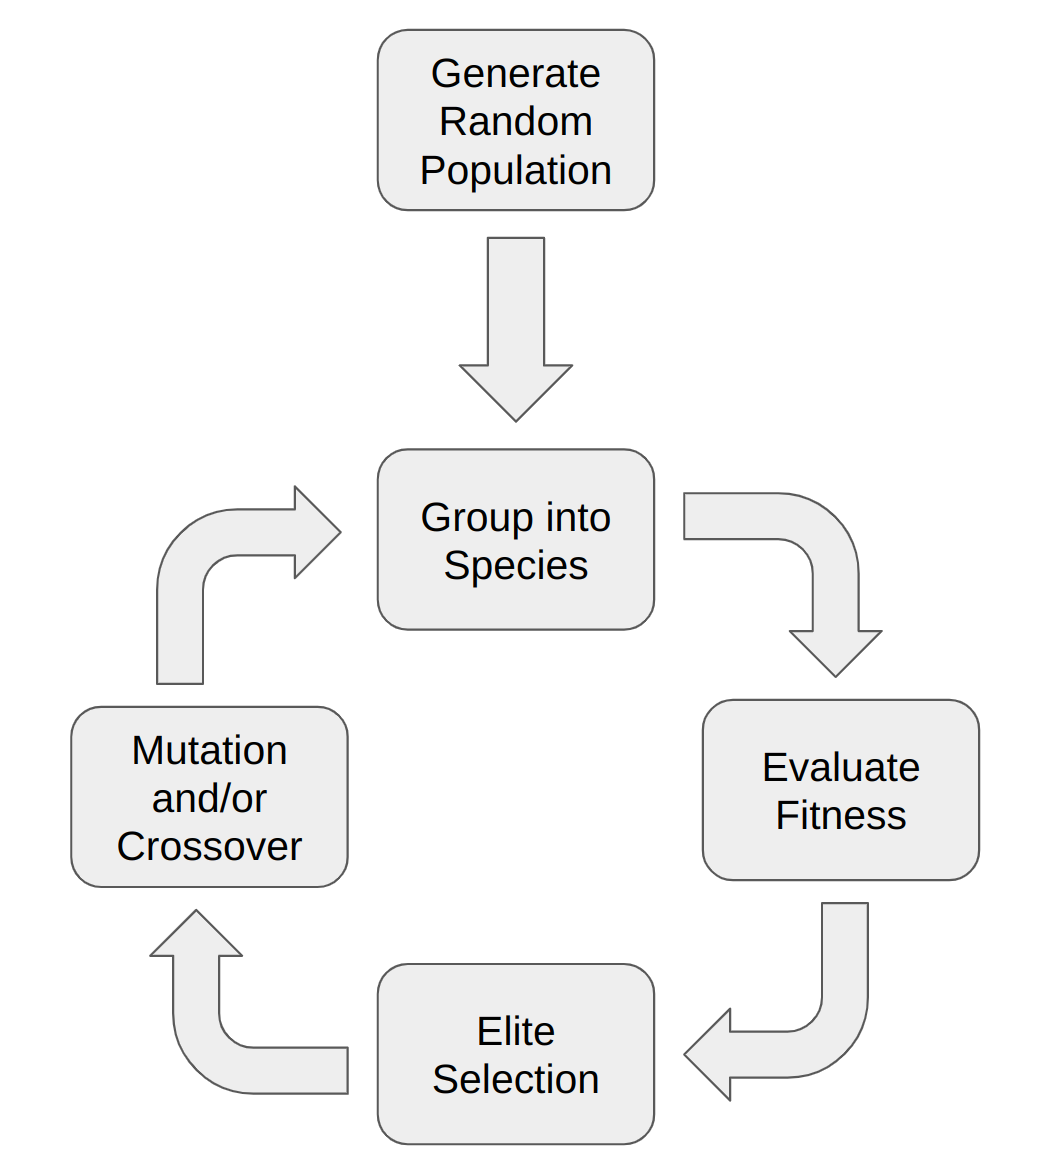
\includegraphics[width=8cm]{images/algo_description_crossover.png}
    \caption[Overview of the evolution algorithm with speciation]{The evolutionary algorithm begins with a population of randomly generated reaction networks. These networks are then grouped into species and their fitness evaluated. The next generation is constructed by first selecting the top performing individuals from each species without modification. The rest of the subsequent generation is populated by networks that are modified by either crossover, mutation, or both. This new generation is then grouped into species based on structural similarity and the process repeats.}
    \label{fig:algo_description_crossover}
\end{figure}

\subsection{Encoding}
Chemical reactions are represented as custom data structures that contain one or two reactants, one or two products, a rate constant, and a boolean value indicating if the reaction is active or inactive. Four types of mass-action reaction are possible: uni-uni (a single reactant to a single product), bi-uni (two reactants form a single product), uni-bi, and bi-bi. A reaction that is active participates in the network that it is part of. An inactive reaction is ``turned off" but remains part of the network as a historical record. It can be activated again or crossed over under certain circumstances. 

A reaction network is a custom data structure consisting of several reactions, initial concentrations for the floating species, and other information to track the individual network. A network can include boundary species (which are assumed to be at a constant concentration throughout the simulation), but boundary species were not used in this study.

\subsection{Mutation}
\label{section: mutation}
There are two types of mutation: rate constant mutation and reaction addition or subtraction. The probability of each of these mutations occurring and the range in which rate constants are mutated can be set by the user. A rate constant mutation can occur in two possible forms. The rate can be increased or reduce by a random percentage, uniformly distributed in a custom range (by default $\pm20\%$), or more rarely a completely new rate constant can be selected, uniformly distributed within a custom range (by default 0.1 to 50). Rate constants were not allowed to become negative, but they did not have an upper bound as previous studies observed that many synthetic oscillating systems rely on a single reaction with an abnormally large rate constant \cite{Tatka2023}.

A reaction mutation is either the addition of a new random reaction or the deletion of an existing reaction, with 50\% chance of each. When a new reaction is added, it is generated randomly with a 
probability of 0.1, 0.4, 0.4, 0.1 for uni-uni, uni-bi, bi-uni, and bi-bi reactions respectively. These probabilities are also configurable. If the randomly generated reaction is already present in the reaction network, the new reaction's rate constant is added to the existing reaction's rate constant. This feature can allow some rate constants to grow to several multiples of the next largest rate constant in the network. When a reaction is deleted, it is ``switched off" and becomes inactive in the network, but is preserved as it can become reactivated under certain circumstances.

\subsection{Crossover}
\label{section: crossover}
During crossover, two parent networks from the same species group are chosen to mate. Analogous to natural evolution, crossover is essential a means of changing more parameters simultaneously and to a greater degree. It injects novelty into the offspring network compared to single mutations. This could either result in faster progress towards a good solution, or could interrupt progress by destroying promising solutions.

\begin{table}
	\centering
    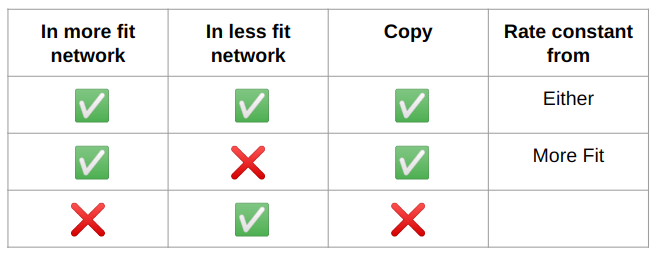
\includegraphics[width=12cm]{images/crossover_table.png}
    \caption[Crossover procedure]{Every reaction in the more fit network is passed down to the offspring network. If it occurs in both parent networks, the rate constant is randomly inherited from one parent or the other.}
    \label{table:crossover_table}
\end{table}

Crossover occurs by examining each reaction in the parent networks. If a reaction is present in both parents, the reaction will be passed down to the offspring network with the rate constant randomly chosen from one parent. If a reaction is present in the more fit parent, but not the less fit parent, the offspring network will inherit the reaction (figure \ref{figure:crossover_example}). If an inherited reaction is currently inactive meaning it was previously deleted during a mutation step), there is a 0.25 probability of the reaction becoming active again. If both parents are equally fit, one is randomly chosen to be the more fit parent (table \ref{table:crossover_table}). 


\begin{figure}
	\centering
    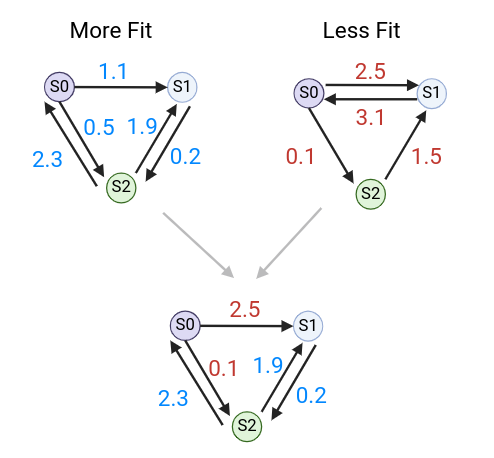
\includegraphics[width=12cm]{images/crossover_example.png}
    \caption[Crossover example]{The topology of the more fit parent is passed to the offspring. Rate constants for reactions that are shared are passed down randomly.}
    \label{figure:crossover_example}
\end{figure}


A second crossover strategy for similar networks was tested in later trials. Networks that were members of the same species and had similar fitness scores (within 5\% of each other) underwent a slightly different crossover process. All reactions that the two networks had in common were passed down to the offspring network with rate constants chosen randomly from one parent or the other. Reactions that occurred in one parent network but not the other had a 50\% chance of being passed down to the offspring network.

\subsection{Speciation}
In many cases, modifying a network, especially through the addition or deletion of reactions, initially makes the system less fit. Without speciation, these innovations seldom last for more than a generation. However, these topological innovations often prove to be an essential step in evolution \cite{stanley_evolving_2002}. For this reason, a speciation strategy is employed to protect innovations and allow them time to optimize. Individuals with similar topologies are grouped into species. Members of a species compete only with each other and not the population at large.  A compatibility distance metric, $\delta$, is used to assign reaction networks to a species, defined as

\begin{equation}
\delta=\frac{M}{N}
\end{equation}
where M is the number of reactions in the larger network that are not present in the smaller network and N is the total number of reactions in the larger network. Two reactions are considered identical if they have the same reactants and products. Rate constants are not considered. If $\delta$ is below the speciation threshold, $\delta_{t}$, the two networks are members of the same species.

For each new generation, networks are assigned to species based on the previous generation's species groups. Each new network is compared to the best network from a species in the previous generation. If $\delta$ is less than the speciation threshold $\delta_{t}$, then the network is assigned to that species. If $\delta$ is greater than $\delta_{t}$, then the network is compared to a randomly selected individual from the next species, etc., until a match is found. If no species is assigned after comparing the network to all species in the previous generation, then a new species is created. 

The speciation threshold $\delta_{t}$ is adjusted with each generation to steer the total number of species towards the target number of species. The target number of species is 10 by default, but can be configured by the user. After each generation the total number of species is counted. If there are more species than the target value, $\delta_{t}$ is increased allowing networks that are more dissimilar to be grouped together. If there are fewer species than the target value, $\delta_{t}$ is decreased. Adapting $\delta_{t}$ as evolution proceeds maintains an optimal number of species. If there are too many species each with a small number of members, there are not enough opportunities to optimize solutions in a small parameter space. Similarly, if there are too few species with several members, the entire parameter space is not adequately explored. 

\begin{equation}
	\delta_{t} = \begin{cases}\delta+\epsilon,& \mbox{if number of species} > N_{s} \\
	\delta-\epsilon,& \mbox{if number of species} < N_{s}
	\end{cases}
\end{equation}

\subsection{Objective Function}

The objective function evaluates how well a candidate model oscillates at the imposed time period, $T$.  Two arbitrary concentrations, $[C]_{1}$ and $[C]_{2}$,  are chosen \textit{a priori}. The fitness score of a network describes how well any of its chemical species approached $[C]_{1}$ at half periods ($T/2$, $3T/2$, $5T/2$,...) and  $[C]_{2}$ at each period ($T$, $2T$, $3T$,...) over the course of 5.5 periods. The candidate model's single chemical species that best approached these points was selected and the fitness was evaluated as the maximum of the reciprocal of the absolute difference between the timeseries data and $[C]_{1}$ or $[C]_{2}$, the ``ideal oscillator" time points, (equation \ref{equation: fitness}). The reciprocal was taken so that higher values represented better fitness, which is necessary for determining the number of offspring for each species in subsequent steps. This objective function has been shown to be an effective means of evolving oscillators in similar and previous work \cite{Paladugu2006, francois_hakim_2004, Tatka2023}. In cases where candidate models could not be simulated, a fitness of 0.0 was assigned resulting in the candidate model's subsequent removal from the population.

\begin{equation}
\label{equation: fitness}
fitness = max(\frac{1}{\sum|ideal - candidate|})
\end{equation}

\subsection{ODE Solver}
During the fitness evaluation phase, reaction networks were converted to systems of ordinary differential equations. These equations were then numerically solved using the DifferentialEquations.jl julia package \cite{DifferentialEquations.jl-2017} and the CVODE solver from the Sundials suite for solving initial value problems \cite{hindmarsh2005sundials}. The CVODE solver was shown to be effective for this application in previous work \cite{Tatka2023}.

\subsection{Reproduction}

Each model species was allocated offspring in proportion with its fitness, with more fit species producing more offspring. The fitness of species was defined as the fitness of its most fit individual. To calculate the number of offspring allocated to each species group, the total fitness of the population was calculated by summing the fitness of each species. Then each species, $s$, was assigned an offspring number proportional to its contribution to the fitness of the entire population (equation \ref{equation: num_offspring}). By default, a single species was only allowed to produce at most 10\% of the subsequent generation in order to prevent a single species from taking over the entire population (but this value could be adjusted by the user). For these reasons, the total number of individuals fluctuated slightly over time.


\begin{equation}
\label{equation: num_offspring}
offspring_{s} = \frac{\sum{fitness_{s}}}{\sum{fitness_{pop}}}*populationsize
\end{equation} 


The reproduction phase began with an elitism selection strategy. The top 10\% of networks in each species were copied to the next generation directly. If a species had 10 or fewer individuals, the single best network was copied without modification to the next generation. Then, the bottom 10\% of networks in each species are deleted. For the remainder of the allocated offspring for each species, a random number, $p$, was generated. If the $p$ was less than the probability of crossover, then two networks from the same species were selected and crossed over to produce a single offspring network. Otherwise a single network was chosen. If $p$ was greater than or equal to 1 - the probability of mutation, the network was mutated. Outside of the elite networks, all networks were either crossed over or mutated. Some were both crossed over and mutated. The probabilities of crossover and mutation could be configured by the user. Probabilities for specific types of mutations are described in section \ref{section: mutation}.

Tournament selection was also explored and can be configured in settings. In this case, two networks from the same species were randomly chosen and the more fit network was then crossed over, mutated, or both. If crossed over, a second network was also chosen by tournament selection (figure \ref{fig:tournament_crossover_diagram}).

\begin{figure}
\centering
    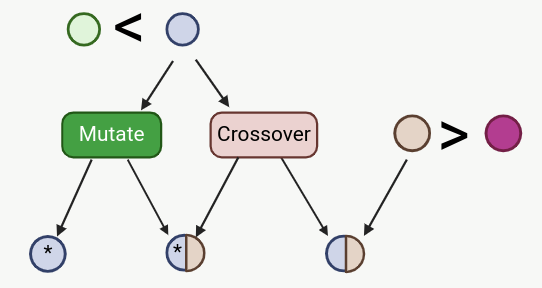
\includegraphics[width=12cm]{images/tournament_crossover_diagram.png}
    \caption[Tournament selection with mutation and/or crossover]{Tournament selection with mutation and/or crossover. Two networks are selected at random and the more fit network of the two undergoes either crossover, mutation, or both. If the network undergoes crossover, a mate network is also chosen by tournament selection.}
    \label{fig:tournament_crossover_diagram}
\end{figure}

\subsection{Output}
The evolutionary algorithm was repeated for a preset number of generations (800 by default) or until the best model reached a predefined fitness level. At this point, the best model from each species was converted to Antimony, a human readable model definition language \cite{Smith2009} and written to a text file along with the model's fitness. All settings were also written out to a JSON file, which could be used without modification to repeat the evolution trial exactly.

The best models from each evolution trial were automatically assessed with a Python script using the Tellurium modeling environment \cite{Choi2018} and RoadRunner simulation software \cite{andy2020}. A model was considered an oscillator if its eigenvalues at steady state contained a positive real number with a nonzero imaginary number and if all concentrations were positive at steady state. Models that met the eigenvalue criteria but had negative steady state concentrations were flagged. Flagged models then underwent a simple automated repair process wherein each reaction was deleted one at a time in an effort to meet the oscillation criteria. Models that met criteria after the simple repair process were counted as oscillators.

In previous work, output networks underwent a post-processing step where superfluous reactions were pruned. This post-processing step was not performed for these experiments so it is possible that many of the evolved oscillating networks have more reactions than are needed to produce oscillatory behavior.

Each evolution trial was run on a single CPU in a linux environment. Often several trials were run in parallel across several CPUs using the cluster computer at University of Washington.

\subsection{Success Metrics}
A single evolution trial was considered successful if it produced a network that oscillated. For each experiment, 700 trials of evolution were performed and the total number of resulting oscillators evaluated. The success rate is the portion of the 700 models that resulted in an oscillator. Experiments sought to maximize this number. Computation time was considered qualitatively in the discussion of results. Often experiments with higher success rates came at the expense of computation time. This metric also did not consider the diversity of the networks produced. For example, a batch of several evolution trials could produce duplicate oscillating networks without penalty. 

\section{Results}
The software was evaluated with multiple hyperparameter settings to assess its ability to generate oscillatory mass-action chemical reaction networks. Each set of hyperparameters were evaluated over 700 evolutionary trials and the success rate recorded. A trial was deemed successful if it generated a network with sustained oscillations, as evaluated by the criteria described previously.


\subsection{Verifying Speciation}
Before evaluating the effects of speciation on evolution, tests were run to verify that speciation was occurring and that the adaptive $\delta$ threshold was maintaining the target number of species. Batches of 700 trials were run for a target number of 1 (no speciation), 5, 10, 30, and 50 species. Figure \ref{fig:avg_num_species} shows that on average, these target numbers were achieved. During the initial generations, the number of species fluctuates more dramatically. This is like due to the fact that while $\delta$ is adaptive, $\epsilon$, the amount by which $\delta$ is changed, is not. During the first several generations, adjustments to $\delta$ tend to over or under shoot the target number of species, likely due to there being large differences between individual networks at first. This over and undershooting causes the number of species to fluctuate before leveling out to the target level after approximately 15 generations.

\begin{figure}
\centering
    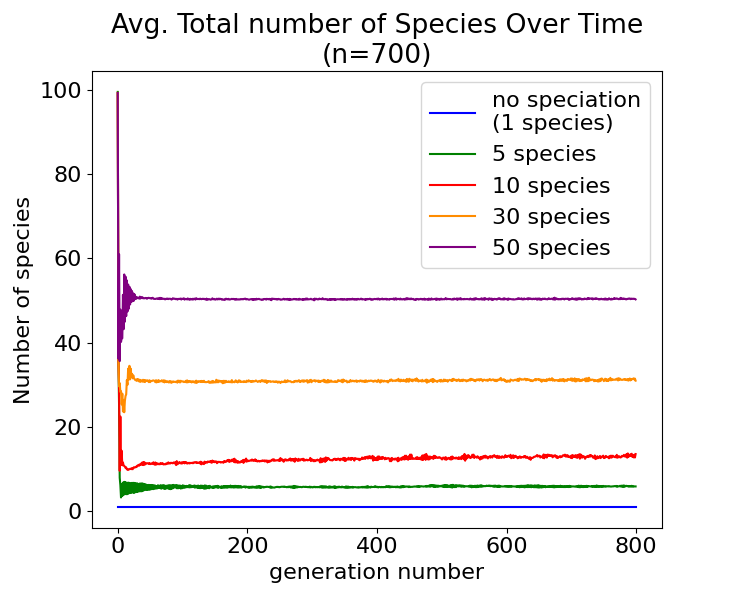
\includegraphics[width=15cm]{images/avg_num_species.png}
    \caption[Average total number of species over time]{Adapting $\delta$ maintains the target number of species without the need to select a value that results in the target number of species through trial and error.}
    \label{fig:avg_num_species}
\end{figure}

The benefit of an adaptive $\delta$ is that the user need only specify the target number of species and $\delta$ will change to accommodate that specification. Without adaptation, $\delta$ must be chosen through trial and error so that it results in the target number of species. For example, in the case of a target species of 10, with an adaptive $\delta$, the total number of species converges to 10 after a few generations and remains there until the end of the trial (figure \ref{fig:adaptive_delta}). With a constant $\delta$, the total number of species is gradually reduced over the course of the trial. In this example, in both cases the success rate was about the same 22\% vs 22.5\% for adaptive and constant $\delta$ respectively. 

\begin{figure}
\centering
    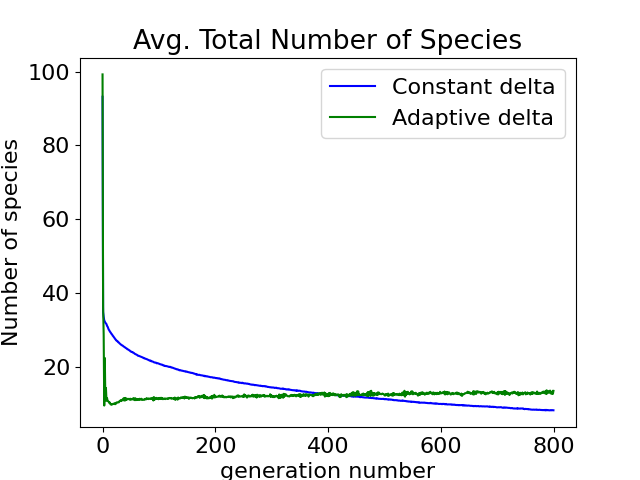
\includegraphics[width=15cm]{images/adaptive_delta.png}
    \caption[Adaptive $\delta$ maintains the target number of species]{Adaptive $\delta$ maintains the target number of species compared to a constant delta.}
    \label{fig:adaptive_delta}
\end{figure}


Although the total number of species remains relatively constant over time, the different species tend to become more similar to each other. The inter-species distance between two species is defined as the distance between the best networks from each species. At each generation, the distance between every combination of 2 species were measured and the average of these measurements recorded. This measurement was performed for batches of 700 trials each for a target of 5, 10, 30, and 50 species. For all four conditions, the average inter-species distance is reduced over time, possibly due to convergence to a single best solution. All three batches started with an average inter-species distance of approximately 0.9, meaning that species differed by an average of 90\% of their reactions. The batch with a target of 10 species converged the most, with an average inter-species difference of approximately 0.55 after 800 generations.   Batches with a target of 30 and 50 species did not converge as much and ended with an average inter-species distance of approximately 0.75 and 0.80 respectively. Larger distances with more species may be due to elitism. With a target of 50 species, at least 50 individuals will be copied to the next generation with no modification. Perhaps lesser networks that otherwise would have been removed if forced to compete with more individuals are allowed to reproduce. Reducing the removal of less fit individuals may allow them to maintain their distances over time. Trials with a target of 5 species converged more rapidly at first, but ultimately did not converge as much as trials with a target of 10 species. Perhaps with too few species, more fit networks dominate the population early on and cause more rapid convergence. However, as evolution progresses, trials with fewer species are less likely to find a good solution and therefor do not further converge.

\begin{figure}
\centering
    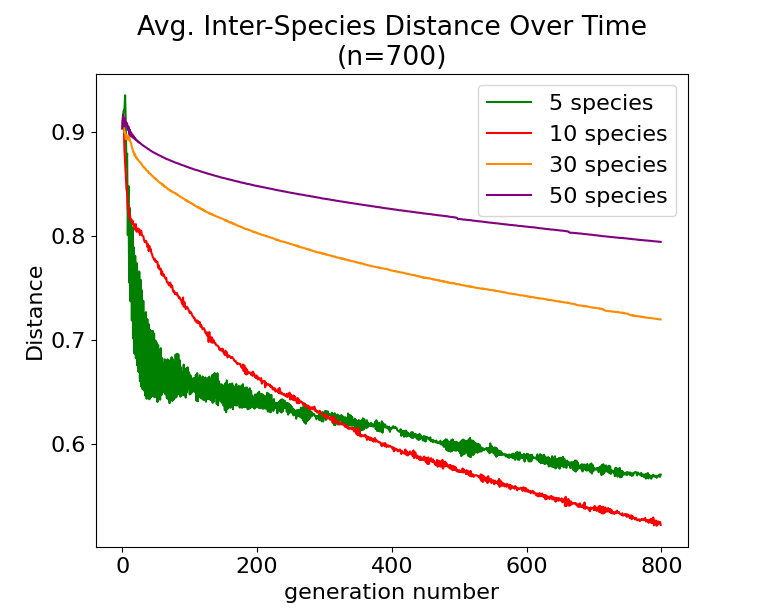
\includegraphics[width=15cm]{images/avg_species_differences.png}
    \caption[Average inter-species distance over time]{Different species become more similar over time.}
    \label{fig:avg_species_differences}
\end{figure}

Next, the average intra-species distances were compared for different target numbers of species. The intra-species distances was computed by averaging the distance between every combination of pairs of networks within a single species. As evolution progresses, species tend to converge on a solution and individuals within a species become more similar. This happens more quickly for trials with larger target species numbers. In order to maintain a larger number of species, the speciation threshold must be stricter, so each species has fewer individuals and individuals within a species are more similar.

\begin{figure}
\centering
    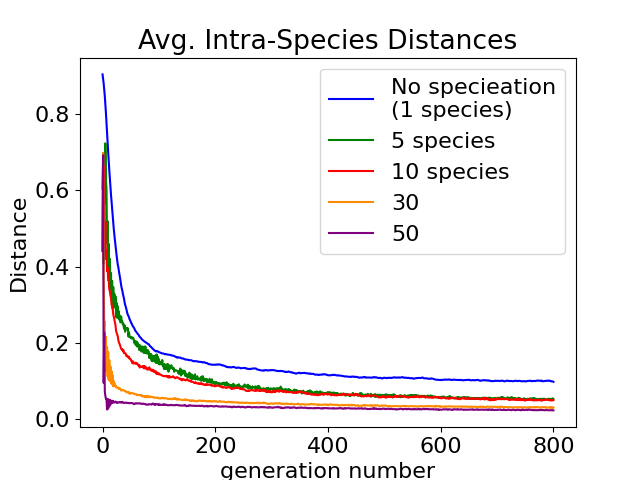
\includegraphics[width=15cm]{images/intraspecies_distance.png}
    \caption[Average intra-species distance over time]{Networks within a species become more similar over time.}
    \label{fig:intra_species_distance}
\end{figure}



\subsection{Speciation Effects}
\label{section:speciation}
In order to test the effects of speciation on population diversity and oscillator success rate, evolution was run without speciation, and with 10 and 30 as the target number of species. When speciation is disabled, the top 10\% of the entire population is passed on to the next generation unmodified and the bottom 10\% of the entire population is deleted. Then mutation is performed on the entire population to populate the remainder of the subsequent generation (crossover was not performed for these experiments). Each network must compete against every other network in the population. To account for fluctuations in population size when speciation is enabled, diversity was measured as the number of unique networks over the total number of networks in the population. A network was considered unique if differed by one or more reactions from all other networks. Reactions are considered different if they differ in product or reactant. Rate constants are not considered in these comparisons. Significance levels were calculated using two-tailed t-tests. 


In trials where no speciation was allowed, the average portion of unique networks was 0.294 $\pm$ 0.035 across 800 generations. This is significantly (p \textless 0.0001) less than the portion of unique networks in evolution trials with a target number of species of 10, 0.344 $\pm$ 0.037 (figure \ref{fig:num_unique_species}).

\begin{figure}
\centering
    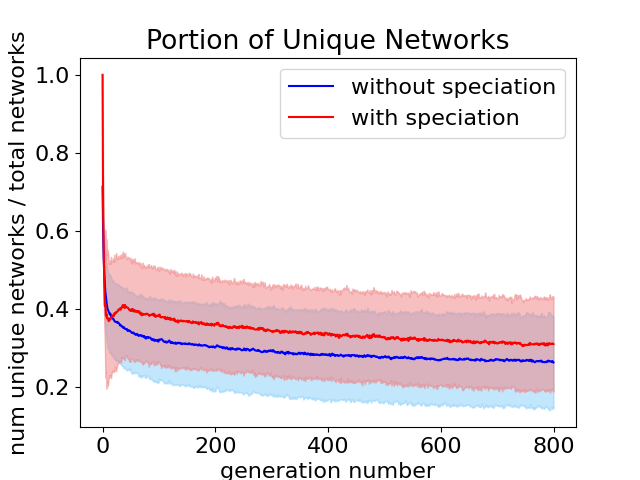
\includegraphics[width=15cm]{images/num_unique_networks.png}
    \caption[Unique networks with and without speciation]{The average portion of unique networks over 800 generations with speciation (red), 0.344 $\pm$ 0.037, and without (blue), 0.296 $\pm$ 0.034. Shading is the 95\% confidence interval.}
    \label{fig:num_unique_species}
\end{figure}

One purpose of speciation was to prevent the most fit network from overtaking the population over time. When a single network dominates the population, there are not enough unique networks to adequately explore the solution space and the evolution algorithm converges on a solution prematurely. To account for fluctuating population sizes when speciation is allowed, the number of copies of the best network divided by the total number of networks was measured at each generation with speciation (with a target species number of 10) and without speciation.  When speciated was enabled, the portion of the population occupied by copies of the most fit network
remained constant with an average portion of best networks of 0.071 $\pm$ 0.008. Without speciation, the portion of best networks rose gradually over time with an average portion of 0.402 $\pm$ 0.079 (figure \ref{fig:portion_best_network}). This shows that speciation effectively prevents a single network from dominating the population (p \textless 0.0001).

\begin{figure}
	\centering
    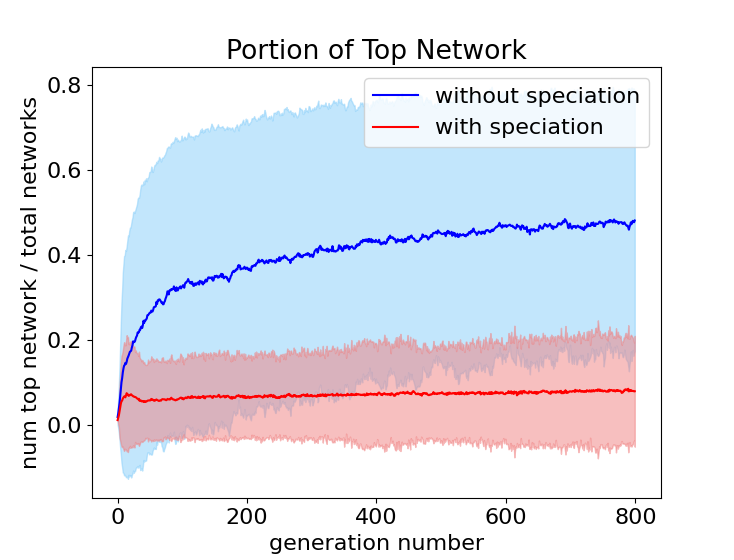
\includegraphics[width=18cm]{images/portion_best_network.png}
    \caption[Portion of top network over time, with and without speciation]{The average portion of best networks over 800 generations with speciation (red), 0.071 $\pm$ 0.008, and without (blue), 0.402 $\pm$ 0.079. Shading is the 95\% confidence interval.}
    \label{fig:portion_best_network}
\end{figure}


Next, the effects of speciation on evolution success rate was evaluated comparing no speciation to speciation with a target species number of 5, 10, 30, and 50 (figure \ref{fig:species_success_rate}. Again, crossover was omitted from these studies. For each speciation level, a batch of 700 trials of evolution were run and the number of oscillators resulting from each batch. Significance levels were calculated using a binomial test. 

With a target species of 10 (the default condition), evolution trials resulted in sustained oscillators at a rate of 0.22 (154/700). Without speciation, the success was significantly reduced (p \textless 0.0001), with oscillators occurring at a rate of 0.12 (83/700). The batch with a target of 30 species also had a success rate of 0.22 (153/700). Increasing the target number of species to 50 significantly (p=0.002) worsened results with a success rate of 0.16 (110/700). Similarly, decreasing the target number of species resulted in a success rate of 0.13 (89/700). This success is still a significant improvement over evolution without speciation (p \textless 0.0001).

Speciation increases the success rate of evolution by sheltering innovations and maintaining population diversity. However, with too many species, there are not enough individuals in any given species to thoroughly explore the space and the success rate is reduced. Similarly, with too few species, there are not enough groups to more broadly explore the solution space and the success rate is reduced.

 
\begin{figure}
	\centering
    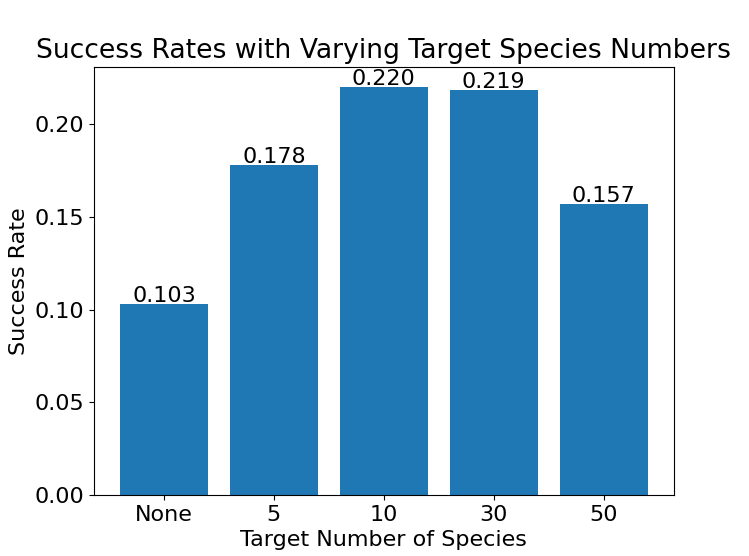
\includegraphics[width=15cm]{images/species_success_rate.png}
    \caption[Evolutionary success rate with varying target species numbers]{Evolution success rate of 700 trials with no speciation and with a target species of 5, 10, 30, and 50.}
    \label{fig:species_success_rate}
\end{figure}

\subsection{Crossover}
To assess the effects of crossover on evolutionary success, batches of 700 evolution trials without crossover and with several type of crossover were compared. None of the crossover batches tested here had better evolutionary success than the batch without crossover. 

First, the crossover technique described previously was compared to a batch with no crossover. Both batches had a target species of 10 and all other parameters in common. The batch with without crossover had 0\% chance of crossover and 100\% chance of mutation.  22\% (154/700) of trials in this batch resulted in oscillators The batch with crossover used the crossover procedure described in the Methods section. The chance of crossover was 75\% and the chance of mutation was 75\%. All networks were either crossed over or mutated ($p_{crossover} + p_{mutation} - p_{crossover} \cap p_{mutation} = 1$). This meant that networks had a 50\% chance of being crossed over and then mutated ($p_{crossover} \cap p_{mutation} = p_{crossover} + p_{mutation} -1$). With these settings, evolution trials with crossover resulted in oscillators at a rate of 17\% (119/700) of the time. This was significantly lower than the success rate without crossover (p = 0.001181).

It was possible that allowing some networks to undergo both crossover and mutation was too much change in a single step and was disrupting any progress towards a solution. In the next batch, networks were only allowed to undergo crossover or mutation (50\% of each), but never both. In this case, 13.7\% (96/700) trials resulted in oscillators, significantly less than both the batch without crossover and the batch with the original crossover method.

In a second attempt to address the problem of too much change, the chance of crossover was reduced from 75\% to 25\%. For this batch, 20.6\% of trials resulted in oscillators. This is significantly better than the batch with a 75\% chance of crossover (p=0.014), but not significantly different than the batch with no crossover. 

With the original crossover method described in \ref{section: crossover}, when two networks have the exact same fitness, one is randomly chosen as the more fit network. It is highly improbable that two networks would have exactly the same fitness, but this prompted the thought that there may be some benefit to more leniently combining two networks with similar fitness scores. For the next batch, networks with a fitness score within 5\% of one another underwent a slightly different crossover method. Like the original crossover method, all reactions that were present in both parent networks were passed to the offspring, with the rate constant chosen randomly from one parent or the other. Reactions that were not shared between the two networks were passed down with a 0.5 probability. As with the original crossover method, reactions that were inactive had a 0.25 probability of reactivation. The success of this batch (16.1\%, 111/700) was no different than the success of the original crossover batch and both were worse than the batch without crossover (p \textless 0.0001).

\begin{figure}
	\centering
    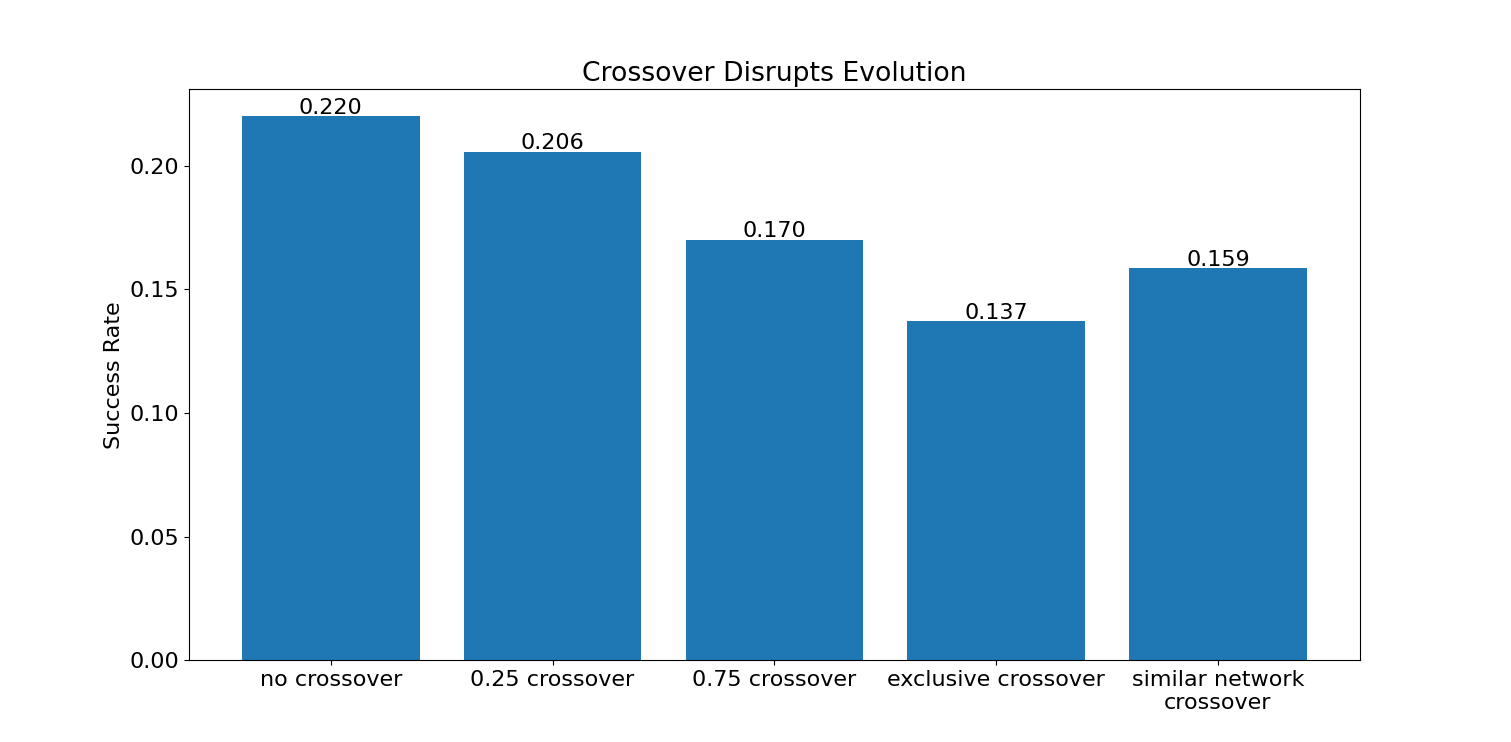
\includegraphics[width=18cm]{images/crossover_success.png}
    \caption[Evolutionary success rate with different crossover strategies]{Evolution success rate of 700 trials with no crossover, 0.25 and 0.75 probability of crossover, 50-50 exclusive chance of crossover or mutation, and 0.75 probability of crossover with more lenient crossover method for networks with similar fitness.}
    \label{fig:crossover_success}
\end{figure}


\subsection{Elitist Selection}
\label{section:elites}
Populating each generations begins with elitist selection. For each species, 10\% of its allocated offspring are unmodified copies of the best networks from the previous generation. In cases where a species is only allocated a single offspring, a mutation is performed on the best network in the species. If the mutation improves the network, the network is passed on to the next generation with the mutation. If the mutation does not improve the network, the unmodified network is passed on to the next generation.

To explore the influence of elitist selection, batches of 700 trials of evolution were run with and without elitism. For batches with elitism, levels of 10, 25, and 50\% were tested\footnote{This is the percentage of the \textit{next} generation that is composed of unmodified, higher fitness models. For example, if a species has 20 members but is only allowed 10 offspring with an elitism rate of 10\%, then the single best network of the 20 will be passed down to the next generation unmodified.}. Eliminating elitism resulted in drastically reduced success rates, with only 1\% (7/700) trials resulting in oscillators. However, in batches with elitism, the percentage of high fitness models copied to the next generation did not result in significantly different success rates. Batches with 10, 25, and 50\% elitism had success rates of 0.220 (154/700), 0.224 (157/700), and 0.197 (138/700) respectively (figure \ref{fig:elitism_success}). It is likely that evolution is driven primarily by the top few individuals. When elitism is removed, these top individuals are not preserved and evolution mostly fails. However keeping more individuals in addition to these top performers does not improve success rates.

\begin{figure}
	\centering
    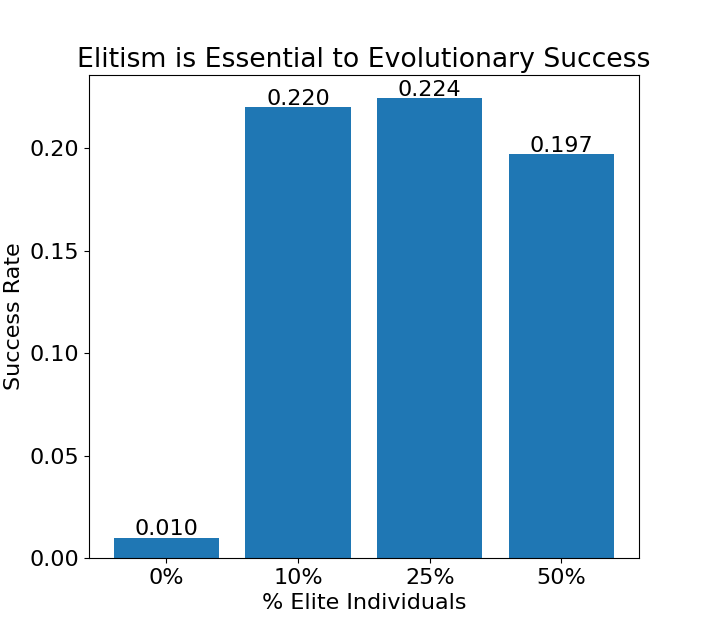
\includegraphics[width=15cm]{images/elitism_success.png}
    \caption[Evolutionary success rate with different levels of elitist selection]{Evolution success rate of 700 trials with no speciation and with a target species of 10, 30, and 50.}
    \label{fig:elitism_success}
\end{figure}


\subsection{Tournament Selection}
After the elite networks were copied to the next generation, the remaining offspring were produced by randomly selecting networks (including the elites, excluding the bottom 10\%) to mutate or crossover. As demonstrated in section \ref{section:elites}, elitism is crucial to the algorithms success. But could a different selection strategy for the non-elite offpsring improve success rate? To test this, tournament selection, with and without speciation, was used to select the non-elite offspring.

Tournament selection involves running several comparisons of a few individuals chosen at random from the population \cite{tournamentselect,  Miller1995}. The best of the subset is chosen for crossover or mutation. It is efficient to code and scales well population size and objective function. In this case, two individuals from the same species were randomly chosen (with replacement) and the individual with the better fitness score was allowed to mutate or crossover and continue to the next generation.

Tournament selection trials with a target species number of 10 and without speciation were compared to trials where non-elite networks were randomly selected. The trial with tournament selection and no speciation performed worst, with only 7.5\% (105/1400) of trials resulting in an oscillator. Interestingly, random selection fared better, with 11.1\% (155/1400) of trials resulting in oscillators (p \textless 0.0001). This result was unexpected, as it would seem that biasing selection towards more fit networks with tournament selection should improve the results. However, it is possible that random selection helped maintain diversity by including less fit networks that ultimately developed into good solutions.

When considering tournament selection with speciation, results improved, with 21.1\% (148/700) of trials resulting in an oscillator. However, this result in not significantly different than random selection with speciation, which resulted in oscillators in 22.0\% of trials (154/700). This bolsters the conclusion that speciation drives evolutionary success more than any other factors explored here.

\begin{figure}
	\centering
    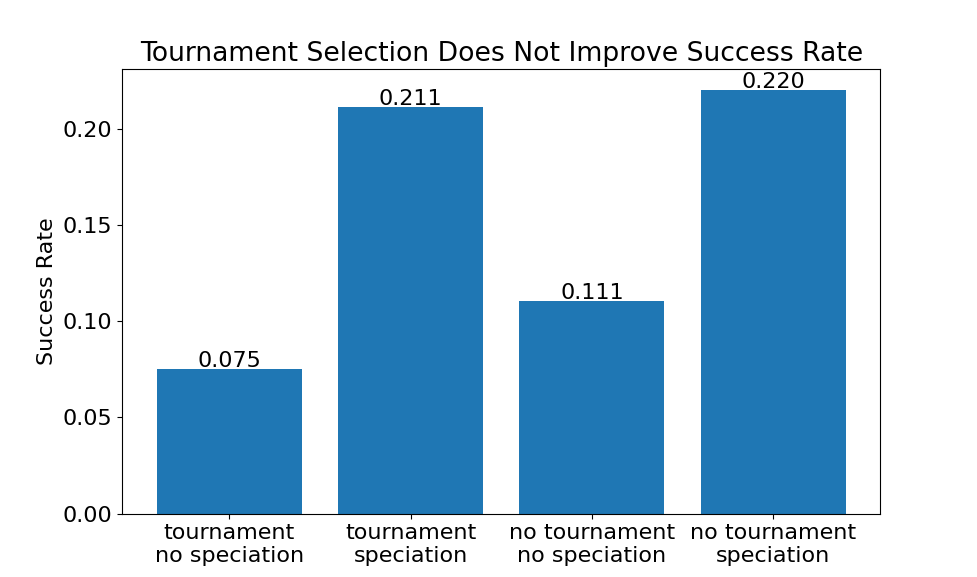
\includegraphics[width=15cm]{images/tournament_speciation.png}
    \caption[Evolutionary success rates with tournament selection and speciation]{Evolution success rate with and without tournament selection and with and without speciation. Speciation influences success rate far more than tournament selection (n=1400 for each no speciation batch, n=700 for speciation batches).}
    \label{fig:tournament_speciation}
\end{figure}

\subsection{Increased Population size}
Unlike other hyperparmaters discussed here, increasing the population size has a direct effect on computation time, as numerically solving the ODEs is the rate limiting step of the algorithm. However, increasing the population size increases the number of individuals exploring the solution landscape and thus increases the chances of finding a good solution. 

When the population size was doubled, from 100 individuals to 200 individuals, evolutionary success significantly improved from 22\% to 26\% (p = 0.012), with 182 of 700 trials producing an oscillator. However, this computation took roughly twice as long. The batch with 100 individuals resulted in 154 oscillators (out of 700 trials). Running this batch twice would result in ~300 oscillators and take roughly the same amount of time as a 200 individual population that produces ~180 oscillators.

Next, a batch with a population of 200 and a target of 20 species was run. For a population of 100, a target species of 10 was shown to result in the highest success rate, so this experiment sought to test if the optimal target number of species scaled with population size. This appeared to be the case as 38.5\% (77/200) trials in this batch resulted in oscillators, a significant improvement over both 200 individuals with 10 species and 100 individuals with 10 species. 

\subsection{More Generations}
Like population size, the number of generations directly effects computation time. However, increasing the number of generations allows more time for the algorithm to discover and optimize solutions and increase evolutionary success. 

The maximum number of generations was doubled, from 800 to 1600, and evolution was run with default parameters: no crossover, 100 individuals, target species of 10. Trials in this batch resulted in oscillators 37\% (74/200) of the time. The fitness of the top network in each generation was tracked and averaged across 200 trials (figure \ref{fig:1600_top_fitness}). After 1600 generations, the average top fitness continues to rise suggesting that the success rate may further increase with more generations. When the number of generations was doubled again, from 1600 to 3200, the success rate was 50\% (100/200). At 3200 generations, the average fitness still did not plateau suggesting that a higher success rate may be possible at the expense of computing time.
 

\begin{figure}
\centering
    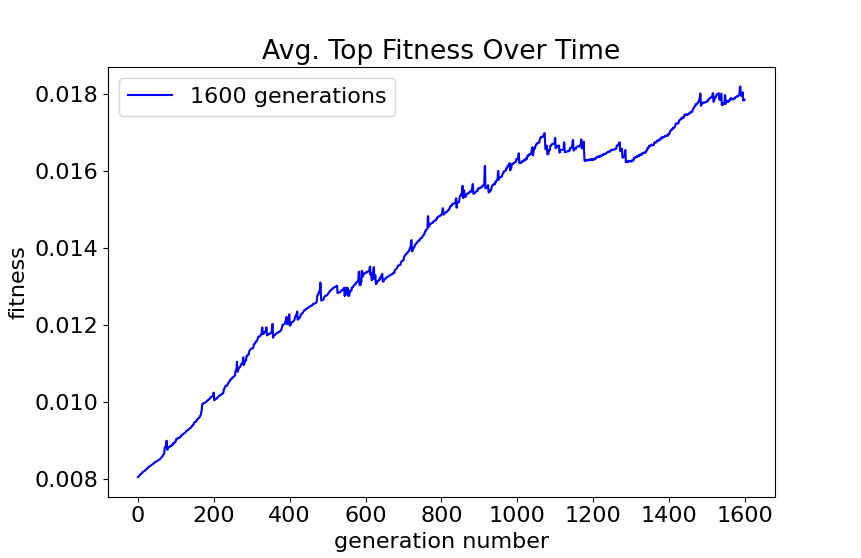
\includegraphics[width=15cm]{images/1600_top_fitness.png}
    \caption[Average top fitness over 1600 generations]{Average fitness of the best network of each generation over 200 trials. Small spikes can likely be attributed to writing out networks with high fitness and discontinuing evolution trials.}
    \label{fig:1600_top_fitness}
\end{figure}


\subsection{Evolving Oscillators with Optimal Settings}
With the insights from these experiments, a batch of 720 trials was run with the best known hyperpamaters. Two hundred individuals with a target of 20 species were evolved over 1600 generations without crossover and without tournament selection. Of the 720 trials, 374 resulted in oscillators for a success rate of 51.9\%. It is likely that increasing the number of generations to 3200 or higher would further increase success rate, but at a cost of computing time.

Examples of time series data generated by randomly selected evolved oscillators are shown in figure \ref{fig:julia_example}. There are a variety of oscillation shapes, amplitudes, and frequencies demonstrating that there are many ways that the objective criteria can be met to produce an oscillator. This suggests that there are a variety of different oscillators in the evolved networks. The networks were not examined for duplicates.

\begin{figure}
\centering
    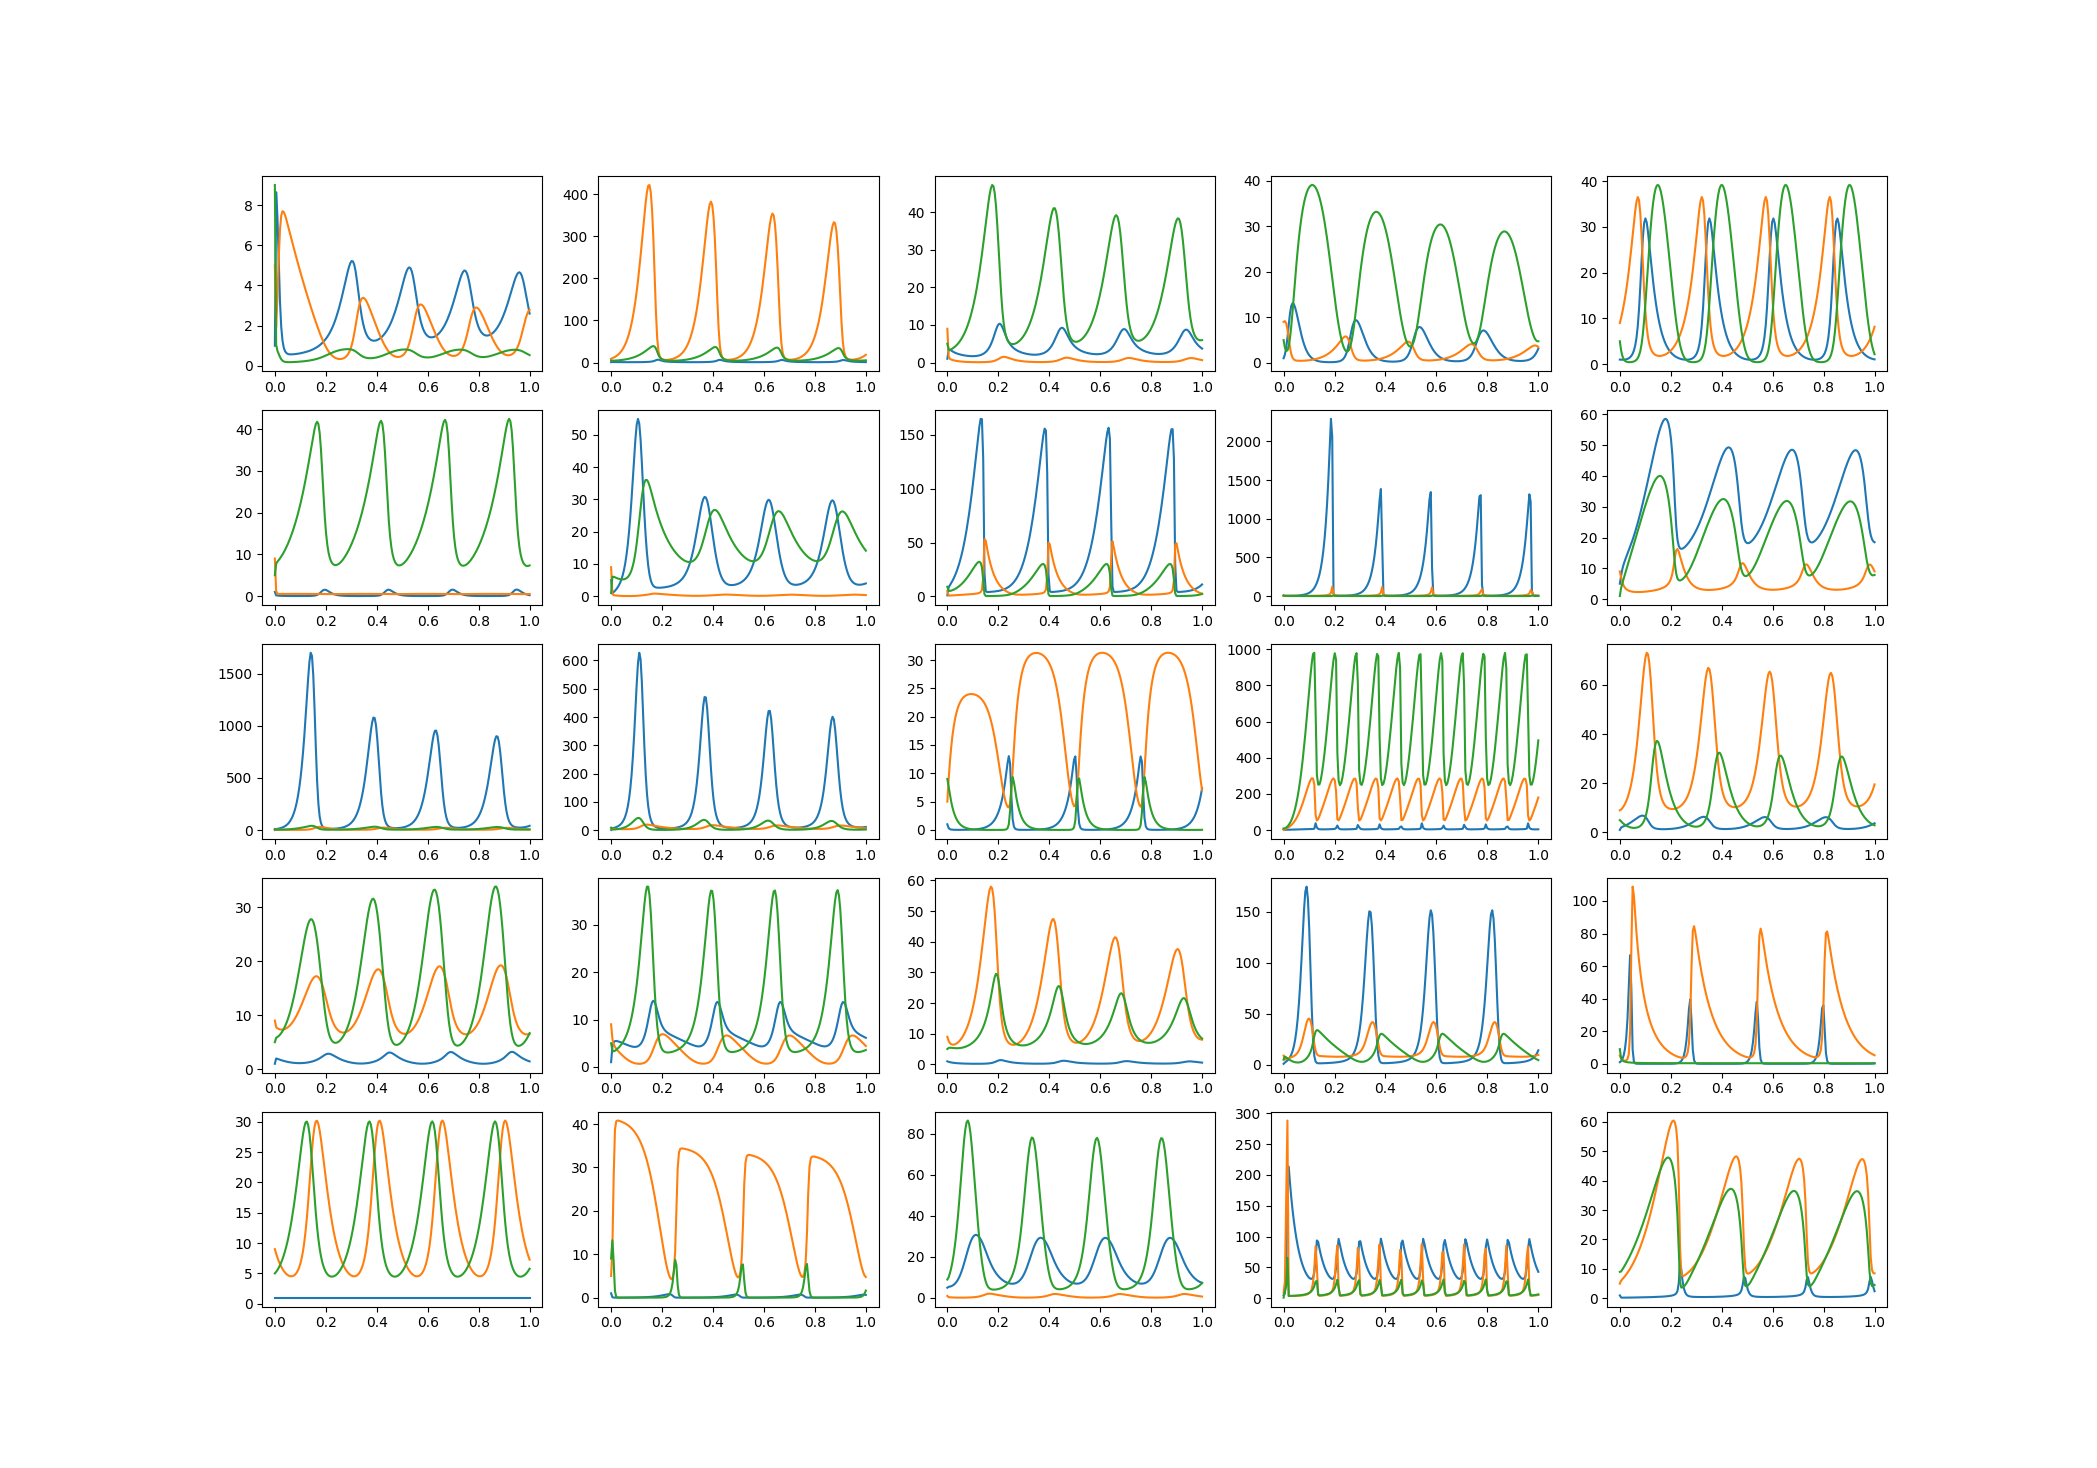
\includegraphics[width=18cm]{images/julia_sample_oscillators.png}
    \caption[Time series data of evolved oscillators]{Time series data from an assortment of evolved oscillators.}
    \label{fig:julia_example}
\end{figure}

Examples of three evolved networks and their timeseries data are shown in figure \ref{fig:examples_networks}. Each network has been processed to remove all reactions that are not necessary for oscillation. The three networks vary in complexity and produce different oscillations in terms of frequency, amplitude, and shape. Despite the difference in complexity, the second and third networks generate a similarly shaped time series. Interestingly, the third network has completly ignored the third chemical species and recreated the Lotka-Volterra predator-prey model.

\begin{figure}
\centering
    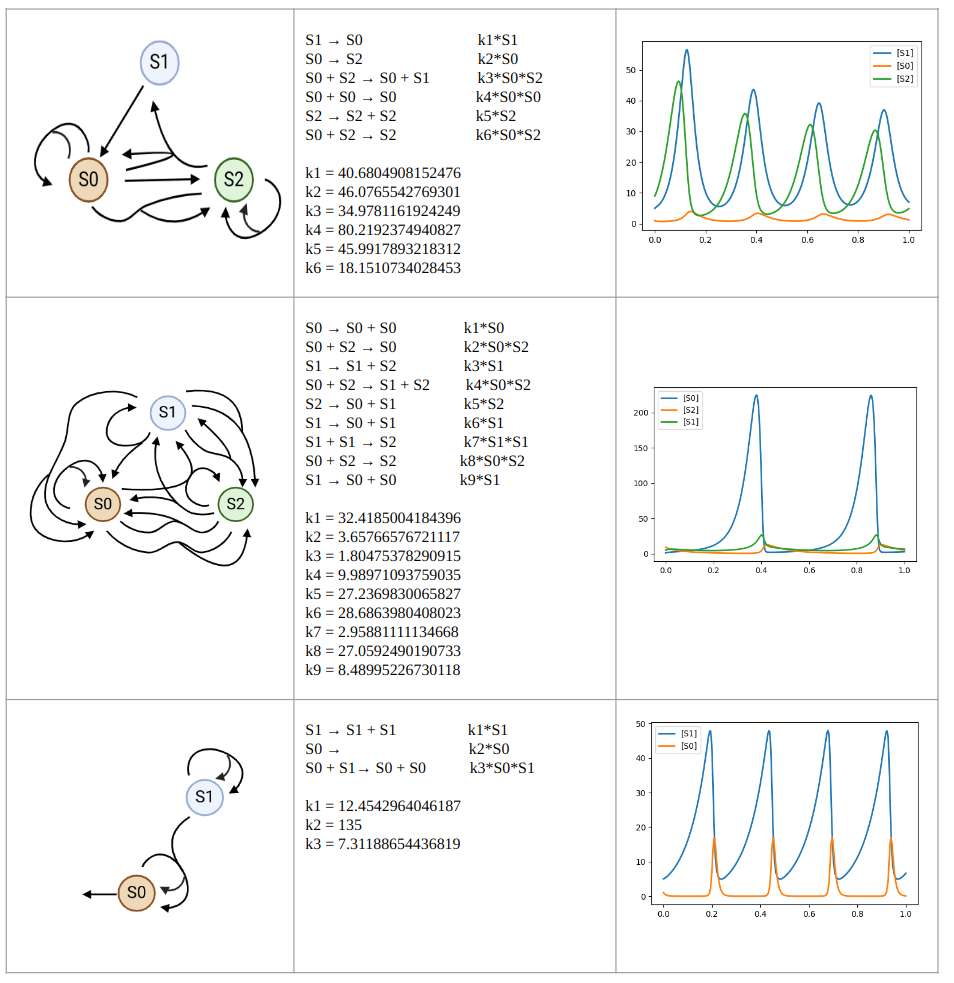
\includegraphics[width=18cm]{images/examples_and_networks.png}
    \caption[Examples of oscillatory networks and their time series]{Examples of oscillatory networks and their time series. The bottom network is the Lotka-Volterra predator-prey network.}
    \label{fig:examples_networks}
\end{figure}

The top fitness values at each generation for five successful evolution trials are shown in figure \ref{fig:fitness_trajectories}. Some networks, such as those shown in blue and purple, make a series of mutations that rapidly improve the fitness. Others develop more gradually. Trials with a fitness value of 0.05 or higher were stopped and saved, but 0.05 is a very conservative cutoff. It is likely that a cutoff value of 0.01 would capture most if not all oscillators. 

\begin{figure}
\centering
    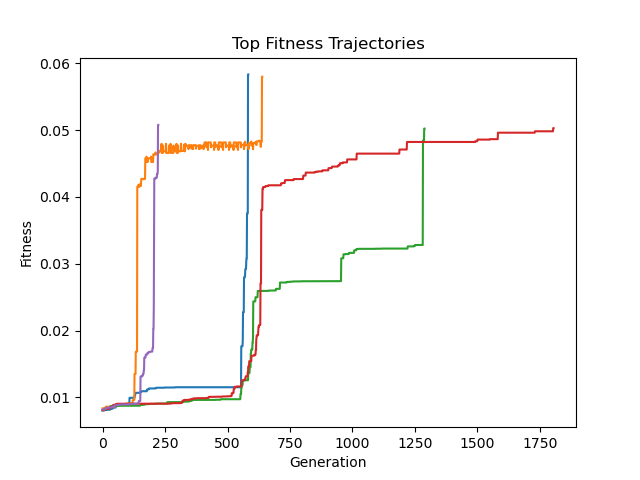
\includegraphics[width=18cm]{images/fitness_trajectories.png}
    \caption[Fitness trajectories of successful evolution trials]{Examples of fitness trajectories of successful evolution trials.}
    \label{fig:fitness_trajectories}
\end{figure}

\subsection{Fitting Time Series Data}
\label{section:fit_timeseries}
Beyond generating oscillators, the ReactionNetworkEvolution.jl software is intended to implement an evolutionary algorithm for more broad systems biology problems. One application could be evolving reaction networks that match time series data. To test if ReactionNetworkEvolution.jl could generate networks to match time series data, a simple, 3 chemical, 5 reaction synthetic network was constructed and its time series data collected (figure \ref{fig:groundtruth}). Then the ReactionNetworkEvolution.jl software was given the time series data as an objective. 

\begin{figure}
\centering
    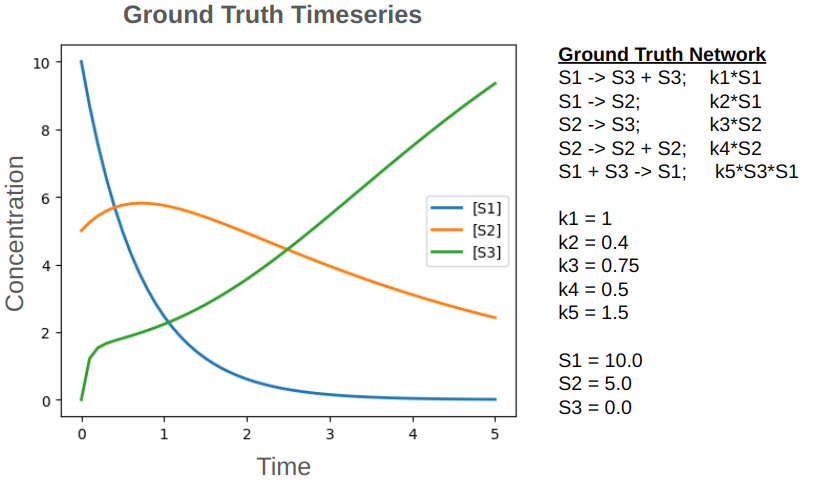
\includegraphics[width=18cm]{images/groundtruth.png}
    \caption[A ground truth synthetic network and its time series]{A synthetic network and its time series data.}
    \label{fig:groundtruth}
\end{figure}

Four hundred trials of evolution were run, each with 1600 generations in an effort to match the ground truth time series data. The time series data of the 12 best evolved networks all closely match the dynamics in the ground truth network (figure figure \ref{fig:12_timeseries}). The best matching time series (top row left of figure \ref{fig:12_timeseries}) is shown overlaid with the ground truth time series in figure \ref{fig:truth_vs_evolved}. The solid lines are data from the ground truth network and the dashed lines are from the evolved network.

\begin{figure}
\centering
    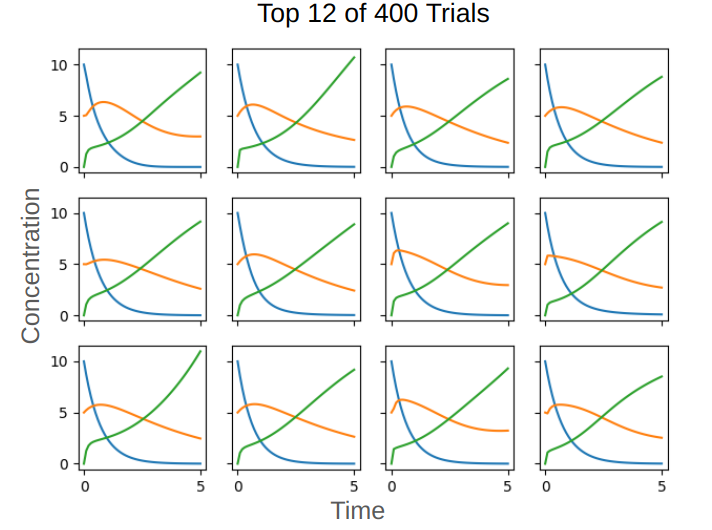
\includegraphics[width=15cm]{images/12_timeseries.png}
    \caption[The 12 trials that most closely matched the time series data]{The 12 trials that most closely matched the time series data.}
    \label{fig:12_timeseries}
\end{figure}

\begin{figure}
\centering
    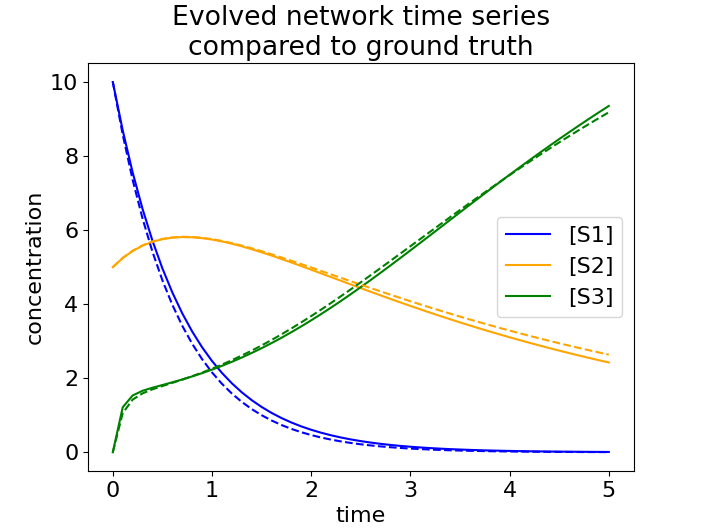
\includegraphics[width=15cm]{images/ground_truth_vs_evolved.png}
    \caption[Time series of the ground truth network compared to the best evolved network]{Time series of the ground truth network (solid lines) compared to the best evolved network (dashed lines).}
    \label{fig:truth_vs_evolved}
\end{figure}

Interestingly, the evolved network that most closely matched the ground truth time series data only had one reaction in common with the original network (figure \ref{fig:evolved_network_structure}). The last reaction, S1 + S3 $\to$ S1, occurred in 10 of the 12 best networks. The next most common was the reaction S2 $\to$ S3, which occurred in 7 of the 12 best networks. All networks that had the reaction S2 $\to$ S3 also had the reaction S1 + S3 $\to$ S1.

\begin{figure}
\centering
    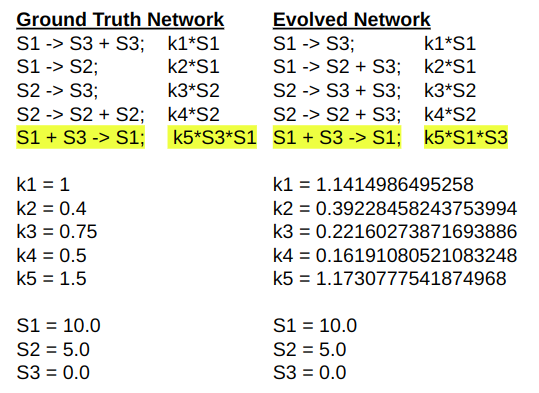
\includegraphics[width=15cm]{images/antimony_truth_evolved.png}
    \caption[The ground truth network compared to the best evolved network]{The ground truth network compared to the best evolved network}
    \label{fig:evolved_network_structure}
\end{figure}

\subsection{Parameter Fitting}
ReactionNetworkEvolution.jl's ability to fit parameters (rate constants) to a given network and time series was tested by supplying it with the ground truth network and time series data from figure \ref{fig:groundtruth}. In this case, ReactionNetworkEvolution.jl implements a more ``classic" evolutionary algorithm, where the topology of the network is fixed and only the parameters are changed. 

The distance metric was modified in order to take advantage of speciation in this context. Previously, the distance metric only took reactions into a account when quantifying the distance between two networks. In a parameter fitting task, all the networks are topologically identical and would all be considered to have a distance of 0 from another an be grouped into a single large species. The average difference  between associated rate constants was added to the distance function. As in the previous distance metric, the first term is the number of reaction in the larger network that are not in the smaller network, divided by the number of reactions in the larger network. For parameter fitting, this will be zero as all the networks are identical. The second term quantifies how different the rate constants are between two models. For reactions that are in both networks, average difference between rate constants for corresponding reactions is multiplied by a weight, W. For this experiment. W was set to 1. W is a configurable setting and is set to 0 by default.


\begin{equation}
\delta=\frac{M}{N} + W\frac{\sum|k_{i1} - k_{i2}|}{N_{shared}}
\end{equation}

\begin{table}
\centering
    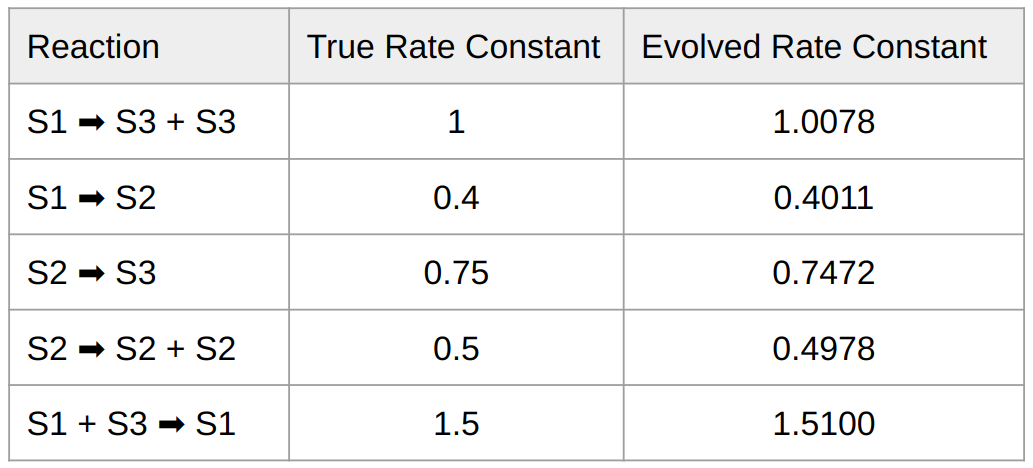
\includegraphics[width=15cm]{images/parameterfit.png}
    \caption[Parameter fitting results]{The evolved rate constants closely match the true rate constants.}
    \label{table:parameterfit}
\end{table}

Evolution was run with 200 individuals, 20 species, 1600 generations, and no crossover. ReactionNetworkEvolution.jl was given the network's topology (without rate constants), and the time series data and tasked with producing rate constants. The best result closely matches the ground truth data (table \ref{table:parameterfit}).

\section{Discussion}
Speciation was shown to significantly benefit evolutionary success by protecting innovations and maintaining evolutionary diversity throughout the process. Fine tuning is necessary to achieve the maximum benefit of speciation. The target number of species must be chosen with consideration of the population size. Additionally, $\delta$ and $\delta$ step sizes may require adjustment for different population sizes, target number of species, and different objectives. 

Elitism is also essential to evolution as it preserves the best individuals of each generation. It pairs well with speciation as it allows the best individuals not just from the whole population but from the each species to be passed on to the next generation. Interestingly, the evolutionary success did not seem to vary with different levels of elitism suggesting that evolutionary progress is driven primarily by the top individuals of each species and that including additional elite networks does not improve success. This seems to be confirmed by the observation that alternative selection strategies for non-elite individuals did not affect evolutionary performance.

Although crossover has shown success in other topological evolution problems \cite{stanley_evolving_2002, dinh_effective_2015}, this was not the case with mass-action networks. Both artificial neural networks (ANNs) and genetic regulatory networks (GRNs) (domains where crossover has been shown effective) have more edges that can more easily be separated from their weights. In both cases, edges simply connect two nodes together. For ANNs, all edges activate the output node and have a weight which increases or decreases the signal strength. GRNs are similar but edges can also be inhibitory. The weights of the edges are not influence by the nodes the edge is connected to. On the other hand, in this work, reactions are analogous to edges and can connect two to four nodes (chemical species). The rate constants are analogous to weights. But unlike weights, the extent to which one node activates another (or the speed at which a reactant becomes a product) is also influenced by the reactant's concentration. That is to say, in the case of mass-action chemical reaction networks, it is far more difficult to isolate subsets of a network and maintain their function. When crossover occurs, it tends to disrupt the finely tuned developing solutions by changing several rate constants simultaneously. This could explain why crossover reduces success in this application despite its utility in other domains. 

Although this algorithm is faster than previous iterations, it still computationally expensive. A single trial of 800 generations and 100 individuals take approximately 90 seconds on average. Given the success rate using these settings, this amounts to approximately 3 minutes per oscillator per CPU. The vast majority of this time is consumed by numerically solving the ODEs. The software uses a custom function to compute the rate of change of each concentration, but the solver is from julia's DifferentialEquations and Sundials libraries, both highly optimized for performance. Additionally, ReactionNetworkEvolution.jl uses strict typing, pre-allocation wherever possible, and hash maps to further improve performance. Although the current implementation of ReactionNetworkEvolution.jl does not make use of parallelization within a single trial, in practice multiple trials can be dispatch to different CPUs using a bash script or job array. Future efforts to improve the success rate are likely to be more fruitful than efforts to increase computational performance.


Using an adaptive speciation threshold, $\delta$, did not directly influence evolutionary success, but it maintained the target number of species which did influence success. Without an adaptive $\delta$, the user would have to manually tune $\delta$ through trial and error to achieve the target number of species. Given the utility of this adaptive feature, it may be useful to implement a similar strategy for other evolutionary hyperparameters. For example, the probability of changing the topology (adding or deleting reactions) versus changing rate constants remains the same throughout the evolutionary process. Early on, it may be useful to change topology more frequently in an effort to find a decent solution. However, later in the process, when a promising solution has been found, it is more useful to modify rate constants in an effort to optimize the solution. Changing topology may be wasted effort and may divert resources that may be better spent optimizing an existing solution. In future iterations of ReactionNetworkEvolution.jl, it may be useful to change the balance of topological versus rate constant mutation over time or as fitness reaches a pre-specified threshold.

Similarly, as evolution progresses and homes in a promising solution, smaller rate constant changes may be necessary to explore a small area in the solution space in more detail. The amount by which rate constants are changed could be adaptively reduced over time, either based on fitness or generation number. 

Another means of more thoroughly exploring a promising solution space as evolution progresses could be altering the metric used to determine the ``distance" between two networks, and thus their species. In the current iteration of ReactionNetworkEvolution.jl, the distance between two networks is entirely determined by the amount of reactions that the two networks do not share with no consideration to the rate constants for shared reactions. Networks with the same topology are considered identical even if rate constants for their different reactions vary by orders of magnitude. Including the differences in rate constants when considering distance could improve evolution by encouraging more thorough explorations of viable solution spaces towards the end of the process. As networks become more topologically similar as evolution progresses, speciation would be driven by differences in rate constants instead of topology. This would direct more resources towards optimizing a decent solution as opposed to continuing to explore the broader solution space.

One flaw of the existing iteration of ReactionNetworkEvolution.jl is the tendency to add extraneous reactions. It appears that more often than not, deleting a reaction reduces fitness whereas adding a reaction may slightly improve fitness. Although there was equal probability of adding and deleting reactions, networks at the end of evolution tended to be much larger (~15 reactions) than at the start (5) reactions. In some cases, this may not be of concern. For example, if the objective is simply to create a population of oscillators, it may not matter that some of them are overly complicated. However, if attempting to gather simple networks to fit time series data, the tendency to over complicate networks could be detrimental. Overfitting by over complicating models (for example, by including too many predictors) is a well-known problem in machine learning. Often, the solution is to penalize machine learning models that use too many features. A similar technique could be implemented here, penalizing candidate networks for each additional reaction. Penalization was briefly explored, but was found to reduce the success rate. Further fine tuning of a fitness function that addresses network complexity may increase the success rate and result in less complex models.

Isomorphism was not considered during of after the evolution process. Networks were only considered similar or identical if both their reactions and the names of the chemical species involved in the reactions matched. However, given the arbitrary naming of the chemical species, it is possible to have two identical networks but with shuffled chemical species names. During the evolution process, this might result in two or more species groups effectively populated with the same network. Similarly, after multiple trials of evolution, there may be a number of oscillators that are isomorphic. 

The issue of isomorphism could be partially addressed in future versions of ReactionNetworkEvolution.jl. During evolution, the names of chemical species could be normalized during fitness evaluation such that the chemical species that most closely matched the input time series was named ``$S_0$," followed by ``$S_1$," and so on. One possible problem with this proposal is that different reaction rates may cause different chemcial species to best match the input time series data despite two networks being topologically identical. 

Identifying isomorphic duplicates after multiple evolution trials could be addressed with multiple pairwise comparisons. For each pair of networks with 3 chemical species, six comparisons between the two networks would be sufficient to identify if two networks are the same despite having shuffled chemical species names. For a population of several oscillators, this would amount to 6${n\choose 2}$ comparisons, where n is the number of oscillating networks to be evaluated. A population of 40 oscillators would require 4,680 comparisons to identify all duplicate networks.

Additionally, the algorithm has demonstrated its ability to produce oscillators, but its ability to match other network behaviors is untested. It successfully generated a network to match simple time series data, but did not manage to recover the network that produced the data. This is expected given the limited amount of information about the network provided to the software. More testing and algorithm development could improve ReactionNetworkEvolution.jl's performance in tasks beyond generating oscillators. 

Another possible application of ReactionNetworkEvolution.jl is parameter fitting. ReactionNetworkEvolution.jl can be supplied with seed networks for the initial population (in lieu of random networks) and time series data. ReactionNetworkEvolution.jl will then use the evolutionary algorithm to explore the parameter (rate constant) space while holding the structure of the network (reactions) constant. This was demonstrated with a simple network, but future work will test ReactionNetworkEvolution.jl's ability to fit parameters for a more complex network. 

\section{Conclusion}
The NEAT algorithm for evolving artificial neural networks was successfully adapted to mass-action chemical reaction networks. The experimental results showed that speciation and elite selection drive evolutionary success. Unlike other domains, crossover negatively impacts evolution of oscillatory mass-action networks. 

The adapted evolutionary algorithm is packaged in a julia module, ReactionNetworkEvolution.jl, for easy use and customization. ReactionNetworkEvolution.jl boasts at least a four-fold improvement in success rates over previous iterations and has considerably better computational performance. Using the default settings, oscillators are generated every three minutes on average using a single CPU.

Future work will explore evolution of more complicated network behaviors. Other directions include improving the algorithm's ability to match time series data when given more information about the network or to suggest what additional information is necessary to narrow down the set of networks that can recapitulate the input time series data.

\chapter{Adapting Credibility Standards to Computational Systems Biology}
\label{chap: review_paper}

\section{Introduction}

\blfootnote{This chapter was originally published as Tatka, L., Smith, L., Hellerstein, J., Sauro, H. Adapting modeling and simulation credibility standards to computational systems biology. J Transl Med 21, 501 (2023).
\\https://doi.org/10.1186/s12967-023-04290-5}As computing power rapidly increases, computational models become more intricate and an increasingly important tool for scientific discovery. In systems biology, where the amount of available data has also expanded, computational modeling has become an important tool to study, explain, and predict behavior of biological systems. The scale of biological models ranges from subcellular components~\cite{Wang2021} to entire ecosystems~\cite{Hassell2021}. Modeling paradigms include mechanistic models, rule-based systems, Boolean networks, and agent-based models~\cite{Bartocci2016}. This review will focus on mechanistic models of subcellular processes.

The Food and Drug Administration (FDA) defines model credibility as ``the trust, established through the collection of evidence, in the predictive capability of a computational model for a context of use''~\cite{FDAguidelines}. Model credibility is important in systems biology as models are used to guide experiments or to optimize patient treatment. This is particularly important given the increasing scale and intricacy of models. Reproducibility, the ability to recreate a model and data \textit{de novo} and obtain the same result~\cite{shin_standards_nodate}, is directly connected to credibility, but even reproducibility remains a challenge. It was recently discovered that 49\% of published models undergoing the review and curation process for the BioModels~\cite{BioModels2020} database were not reproducible primarily due to missing materials necessary for simulation, the availability of the model and code in public databases, and lack of documentation~\cite{tiwari_reproducibility_2021}. With some extra effort, an additional 12\% of the published models could be reproduced.  A model that cannot be reproduced is not credible. 

Due to the increasing importance of computational models in scientific discovery, the National Aeronautics and Space Administration (NASA), the FDA, and other regulatory bodies have developed standards to assess the credibility of models~\cite{babula_nasa_2009,FDAguidelines,Shepard2015}. These standards are somewhat vague and generally qualitative to accommodate the broad scope of models in these fields. However, mechanistic models in systems biology are relatively narrow in scope and are supported by a variety of standards for model encoding, annotation, simulation, and dissemination potentially enabling the development of a credibility standard for mechanistic systems biology models.

In this chapter, we discuss current systems biology modeling standards that could aid in the development of credibility standards, examine existing credibility standards in other scientific fields, and propose that current standards in systems biology and other fields could support the development of a credibility standard for mechanistic systems biology models.

\section{Current Standards in Systems Biology}

Klipp et al. describe standards as agreed-upon formats used to enhance information exchange and mutual understanding~\cite{Klipp2007StandardsIC}. In the field of systems biology, standards are a means to share information about experiments, models, data formats, nomenclature, and graphical representations of biochemical systems. Standardized means of information exchange improve model reuse, expandability, and integration as well as allowing communication between tools. In a survey of 125 systems biologists, most thought of standards as essential to their field, primarily for the purpose of reproducing and checking simulation results, both essential aspects of credibility~\cite{Klipp2007StandardsIC}.

A multitude of standards exist in systems biology for processes from annotation to dissemination. Although there is currently no widely used standard for model credibility, the development of this standard is likely to depend on existing systems biology standards, just as standards for model simulation are dependent on standards for model encoding. This section will summarize current standards relevant to model credibility including standards for ontology, encoding, simulating, and disseminating models.  Although standards also exist for graphical representation of systems biology models (SBGN)~\cite{SBGN} and representation of simulation results (SBRML)~\cite{SBRML}, these will not be discussed here as they are less relevant to the future implementation of model credibility standards. 

\subsection{Model Representation}
Having a commonly understood language for describing a model is essential in exchange, reproducibility, credibility. Without a common language to describe models, they cannot be simulated across different platforms or freely shared. For this reason, systems biology model representation has become standardized using XML-based languages SBML~\cite{Klipp2007StandardsIC, machado_modeling_2011}, CellML~\cite{CellML}, and BioPAX~\cite{demir_biopax_2010}. NeuroML~\cite{Gleeson2010}, similar to SBML and CellML, is used to represent neuronal models, but is beyond the scope of this proposal.  

\subsubsection{SBML}

The most widely used model format is SBML (Systems Biology Markup Language)~\cite{SBML, Finney2003, Klipp2007StandardsIC, machado_modeling_2011}. SBML is a XML-based language for encoding mathematical models that reproduce biological processes, particularly biochemical reaction networks, gene regulation, metabolism, and signaling networks~\cite{SBML, Kohl2011}. SBML encodes critical biological process data such as species, compartments, reactions, and other properties (such as concentrations, volumes, stoichiometry, and rate laws) in a standardized format. Annotations can also be stored in the SBML format. With its support by over 200 third party tools and its ability to easily convert to other model formats, SBML is the de facto language for systems biology models~\cite{Kohl2011, machado_modeling_2011}.

SBML models are composed of entities, such as species, located in containers that can by acted upon by processes that create, destroy, or modify~\cite{Keating2020}. Other elements allow for the definition of parameters, initial conditions, variables, and mathematical relationships. The SBML language is structured as a series of upwardly compatible levels, with higher levels incorporating more powerful features. Versions describe the refinement of levels. Most recently, SBML level 3 introduced modular architecture consisting of a set of fixed features, SBML level 3 core, and a scheme for adding packages that augment the core functionality. This allows for extensive customization of the language while enabling reuse of key features. Currently, eight packages are part of the SBML 3 standard. These packages extend the capability of SBML such as enabling descriptions of uncertainties in terms of distributions~\cite{Smith2020}, allowing for the encoding, exchange, and annotation of constraint-based models~\cite{Olivier2018},  rendering visual diagrams~\cite{Gauges2015}, among many others~\cite{Keating2020}. 


\subsubsection{CellML}
Similar to SBML but broader in scope, CellML is also an XML-based language for reproducing mathematical models of any kind, including biochemical reaction networks~\cite{Beard2009}. CellML models do not encode biological information explicitly in the model, but instead consist of mathematical formulations of biological processes~\cite{Wimalaratne2009}. This feature of the CellML language increases flexibility enabling the description of a wide variety of biological processes. CellML models are composed of several interconnected components~\cite{Mesiti} with each component containing at least one variable that is associated with physical units.  This enables CellML processors to automatically check equations for dimensional consistency. 


Both CellML and SBML use almost identical mathematical expressions in MathML, an international standard for encoding mathematical expression using XML~\cite{Caprotti1999}. CellML explicitly encodes all mathematics, such as ODEs~\cite{Smith2013}. It is more versatile than SBML, capable of describing any type of mathematical model. SBML defines reaction rates, which can be used to build rate rules and ODEs~\cite{Hucka2015}. There is more third party support for SBML and it is a semantically richer language compared to CellML~\cite{machado_modeling_2011, Smith2013}.


\subsubsection{BioPAX}
BioPAX (Biological Pathway Exchange) is an ontology, a formal systems of describing knowledge that structures biological pathway data making it more easily processed by computer software~\cite{demir_biopax_2010}. It describes the biological semantics of metabolic, signaling, molecular, gene-regulatory, and genetic interaction networks~\cite{demir_biopax_2010}. Whereas SBML and CellML focus on quantitative modelling and dynamic simulation, BioPAX concentrates primarily on quantitative processes and visualization~\cite{demir_biopax_2010, buchel_qualitative_2012}.  

BioPAX contains one superclass, Entity. Within the Entity superclass, there are two main classes: PhysicalEntity and Interaction. PhysicalEntity describes molecules, including proteins, complexes, and DNA, while the Interaction class defines reactions and relationships between instances of the PhysicalEntity class. Interactions can be either Control or Conversion, both of which are divided into several more detailed subclasses~\cite{demir_biopax_2010, buchel_qualitative_2012}. Like SBML, BioPAX is released level-wise with level 1 describing interactions, level 2 supporting signaling pathways and molecular interactions, and level 3 enabling the description of gene-regulatory networks and genetic interactions.

\subsection{Annotation}

As models grow more numerous and complex, there is an increasing need for a standardized encoding format to search, compare, and integrate them. While standards such as SBML and CellML provide information on the mathematical structure of a model, there is no information as to what variables and mathematical expressions represent. Simple textual descriptions of these representations are subject to errors and ambiguity and require text-mining for computational interpretation~\cite{Curtout2011}. Standardized metadata annotations address these issues by capturing the biological meaning of a model's components and describing its simulation, provenance, and layout information for visualization. The use of annotations improves model interoperability, reusability, comparability and comprehension~\cite{Gennari2021}. Annotations are enabled by systems biology specific ontologies~\cite{Wimalaratne2009} which define a common vocabulary and set of rules to unambiguously represent information~\cite{Noy2001OntologyD1}.
 
To avoid accounting for a variety of annotation formats and approaches, standard annotation protocols are necessary~\cite{Gennari2021}. However, despite the numerous standards and tools, annotation remains a challenge. For example, the ChEBI database~\cite{Hastings2015} has approximately 1,000 annotations for glucose. While more than one entry for each annotation can serve a purpose (some users may prefer to be more abstract in their annotations), this adds to the challenge of defining the purpose of a model and, therefore its credibility.  Additionally, annotations can be obsolete, inappropriate or incorrect, or provide insufficient information. Evaluating the quality of annotations would be essential in any credibility assessment for systems biology models. Some tools already exist for this purpose, such as SBMate~\cite{Shin2021}, a python package that automatically assesses coverage, consistency, and specificity of semantic annotations in systems biology models.

\subsubsection{MIRIAM}
 MIRIAM (Minimum Information Requested in the Annotation of Biochemical Models)~\cite{novere_minimum_2005} was developed to encourage the standardized annotation of computational models by providing guidelines for annotation. The MIRIAM guidelines suggest that model metadata clearly references the relation documentation (e.g. a journal article), that the documentation and encoded model have a high degree of correspondence, and that the model be encoded in a machine-readable format (such as SBML or CellML). Annotations should also include the name of the model, the citation for its corresponding journal article, the contact information of the creators and date of creation, as well as a statement about the terms of distribution. Additionally, models should have accurate annotations that unambiguously links model components to corresponding structures in existing open access bioinformatics resources. The referenced information should be described using a triplet, {data collection, collection-specific identifier, optional qualifier} and expressed as a Uniform Resource Identifier (URI), a unique sequence of characters that identifies a resource used by web technologies~\cite{berners2005uniform}. The optional qualifier field is used to describe relationships between the model constituents and the piece of knowledge with language such as ``has a'', ``is a version of'', ``is homologous to'', etc. 
 
\subsubsection{Systems Biology Ontology (SBO)}
SBO (Systems Biology Ontology) describes entities used in computational modeling~\cite{SBO, Curtout2011}. It defines a set of interrelated concepts used to specify the types of components specified in a model and their relationships to one another. Annotation with SBO terms allows for unambiguous and explicit understanding of the meaning of model components and enables mapping between elements of different models encoded in different formats~\cite{Curtout2011}. Both SBML and CellML support annotation with SBO terms.  SBML elements contain an optional sboTerm attribute~\cite{Curtout2011, Hucka2015, Wimalaratne2009}. 


\subsubsection{OMEX}
In order to harmonize the metadata annotations across models encoded in various formats, Gennari \textit{et al.}, with the consensus of the COMBINE (Computational Modeling in Biology Network) community, developed a specification for encoding annotations in Open Modeling Exchange (OMEX)-formatted archives. The specification describes standards for model component annotations as well as for annotation at the model-level, and archive-level~\cite{Gennari2021}. The specification describes annotation best practices and addresses annotation issues such as composite annotations, annotating tabular data and physical units, as well as provides a list of ontologies relevant to systems biology. Implementation of these specifications is aided by LibOMexMeta, a software library supporting reading, writing, and editing of model annotations. It uses Resource Description Framework~\cite{Decker2000} (RDF), an XML-based standard format for data exchange on the web, for representing annotations. It also makes use of several standard knowledge resources describing biology and biological processes such as ChEBI~\cite{Hastings2015}, a dictionary of small chemical compounds, and UniProt~\cite{Apweiler2004}, a database of protein sequence and functional information.

\subsubsection{Annotation in CellML and SBML}
 Both CellML and SBML have their own annotation protocols based on RDF~\cite{Wimalaratne2009}. The CellML language uses its own ontology for model annotation, a necessity due to the flexibility of the language~\cite{Beard2009}. The CellML Metadata Specification was developed parallel to the CellML language~\cite{Wimalaratne2009}. CellMLBiophysical/OWL ontology is composed of two categories: physical and biological~\cite{Wimalaratne2009}. The physical ontology describes physical quantitative information and concepts captured in the model's mathematical expressions. It is subdivided into processes, such as enzyme kinetics, ionic current, and rate constants, and physical entities, such as area, concentration, volume, and stoichiometry. The biological ontology provides description for processes, entities, the role of an entity in relation to a process, and the specific location of the entity in a biological system. Bioprocesses are divided into three subclasses: biochemical reactions, transport, and complex assembly. Biological entities include proteins, small molecules, and complexes. The biological roles subclass is composed of modifiers, reactants, and products. 

%Hacky BS spacer before BioModels.net to prevent text from flowing into margins
SBML also facilitates MIRIAM compliant annotation using RDF)~\cite{Swainston2009,Decker2000}. Annotations use \\BioModels.net~\cite{LeNovere2006} qualifier elements embedded in XML form of RDF~\cite{Hucka2019}. Each annotation is a single RDF triple consisting of the model component to annotate (subject), the relationship between the model component and the annotation term (predicate), and a term which describes the meaning of the component (object). These terms come from defined ontologies, such as SBO~\cite{SBO}. RDF annotation is supported by the software libraries libSBML~\cite{libSBML} and JSBML~\cite{Rodriguez2015}.



\subsection{Simulation and Parameter Estimation}
Information about a model alone is insufficient to enable efficient reuse. A variety of advanced numerical algorithms and complex modeling workflows make the reproduction of simulations challenging. Many modelers reproduce simulations by reading the simulation description in the corresponding publication~\cite{waltemath_minimum_2011}. This is time consuming and error prone and the published description of a simulation is often incomplete or incorrect. For these reasons, it is essential to define and include information necessary to perform all simulations.

\subsubsection{MIASE}
Guidelines for the Minimum Information About a Simulation Experiment (MIASE) were introduced to specify what information should be provided in order to correctly reproduce and interpret a simulation~\cite{waltemath_minimum_2011}. MIASE is a set of rules that fall into three categories: information about the model used in the simulation experiment must be listed in a way that enables reproduction of the experiment; all information necessary to run any step of the experiment must be provided; all information needed to post-process data and compare results must be included.  Along with MIRIAM~\cite{novere_minimum_2005} guidelines, MIASE compliance guarantees that the simulation experiment is true to the intention of the original authors and is reproducible. 

\subsubsection{KiSAO}
KiSAO (Kinetic Simulation Algorithm Ontology) is an ontology used to describe and structure existing simulation algorithms~\cite{Zhukova2011, Curtout2011}. It consists of three main branches, each with several subbranches. The first branch is Kinetic simulation algorithm characteristics, such as the type of system behavior or type of solution. The second in the kinetic simulation algorithm such as Gillespie or accelerated stochastic simulation. The third branch is kinetic simulation algorithm parameters which describe error and granularity, among other characteristics. 

\subsubsection{SED-ML}
Simulation Experiment Description Markup Language (SED-ML) is software independent, XML-based format for encoding descriptions of simulation experiments and results~\cite{bergmann_simulation_2018, Smith2021simulation}. To help modelers comply with MIASE rules, SED-ML describes the details of simulation procedures, including what datasets and models to use, which modifications to apply to models, which simulations to run on each model, how to post-process data, report, and present results can all be encoded~\cite{waltemath_minimum_2011}. Each algorithm mentioned in a SED-ML file must be identified by a KiSAO term~\cite{Curtout2011}. PhraSED-ML was developed to enable modelers to encode human readable SED-ML elements without the use of specialized software~\cite{choi_phrased-ml_2016}.

\subsubsection{PEtab}
Parameter estimation is common in modeling and simulation, which often requires running multiple simulations to scan the suitability of several parameter sets.  Although many parameter estimation toolboxes exist, they each use their own input formats. The lack of a standardized format makes it difficult to switch between tools, hindering reproducibility~\cite{Schmiester2021}.  PEtab is a parameter estimation problem definition format consisting of several files containing information necessary for parameter estimation, including the model (in SBML format), experimental conditions, observables, measurements, parameters, and optional visualization files~\cite{Schmiester2021}. A final PEtab problem file links all other files to form a single, reusable, parameter estimation problem. Following the success of PEtab, parameter estimation functionality was added to SED-ML~\cite{Smith2021simulation}.

\subsection{Dissemination}
Model reproducibility best practices describe dissemination as an essential part of reproducibility~\cite{porubsky_best_2020}. Sharing all model artifacts and documentation on open-source repositories allows independent researchers to reproduce, reuse, and understand the model. Several guidelines and archive formats have been developed to ensure that all relevant information necessary to reproduce a modeling result is easily accessible to the public.


\subsubsection{MIRIAM Curation Guidelines}
In addition to annotation guidelines, MIRIAM also provides guidelines for model curation, the process of collecting and verifying models. The aim of MIRIAM guidelines is the ensure that model is properly associated with a reference description (e.g. a journal article) and that it is consistent with that reference description, meaning that it reflects the biological process listed in the reference description. The model must be encoded in a public, machine-readable format such as SBML or CellML and comply with the associated encoding standard. The encoded model must be simulatable, including quantitative values for initial conditions, parameters, and kinetic expressions, and must reproduce relevant results when simulated~\cite{novere_minimum_2005}.

\subsubsection{FAIR}
More recently, the FAIR guidelines were published to improve the ability of computers to \textbf{F}ind, \textbf{A}ccess \textbf{I}nteroperate, and \textbf{R}euse models~\cite{Wilkinson2016} with minimal human interaction. FAIR defines characteristics that data resources should possess to assist with discovery and reuse by third-parties. Unlike most data management and archival guidelines, FAIR is a set of high-level, domain-independent guidelines that can be applied to a variety of digital assets. Each element of the FAIR principle is independent. 

For a model to be ``findable," it should be easy to find for both humans and computers. This requires describing and annotating data and metadata with unique identifiers that are registered or indexed in a searchable resource. Once the user finds the relevant model, it should be accessible: data and metadata should be retrievable by their identifiers using standard communications protocol. Metadata should remain accessible even when data are no longer available. Interoperability refers to the integration with other data and the ability to operate with various applications and workflows. This is enabled by the use of broadly applicable languages for model representation and annotation. As the ultimate goal of FAIR is to enable the reuse of data, the guidelines dictate that data and metadata should be associated with detailed provenance, meet domain-specific community standards (such as COMBINE archive format described below), and released with clear and accessible data usage license.


\subsubsection{COMBINE Archives}
COMBINE (COmputational Modelling in BIology NEtwork) is a formal entity that coordinates standards in systems biology.  To assist in this coordination, a MIRIAM compliant system for sharing groups of documents regarding a model was developed called the COMBINE Archive~\cite{schreiber_specifications_2020}. The archive is encoded in OMEX (Open Modeling Exchange format) and the archive itself is a ``ZIP" file. A COMBINE archive could contain files in several different standard formats including SBML, SBOL, and SED-ML among others. Additionally, every COMBINE Archive contains at least one file titled \textit{manifest.xml} that contains a list of all the files comprising the archive and describing their locations. An archive also may contain a metadata file, ideally conforming to MIRIAM and MIASE guidelines. The inclusion of all necessary protocols and data needed to implement a model enables distribution of models via a single file encouraging reuse and improving reproducibility~\cite{bergmann_combine_2014}.



\section{Credibility Guidelines in Systems Biology}

Although no standard for model credibility in systems biology exists, there are general guidelines aimed at improving the trustworthiness of models developed by the Committee on Credible Practice of Modeling and Simulation in Healthcare, a group formed by the U.S. National Institutes of Health~\cite{erdemir_credible_2020}. The purpose of these guidelines is to encourage the credible use of modeling and simulation in healthcare and translational research. These guidelines are qualitative and share many components with best practices for reproducibility. The term ``credible" was defined as  ``dependable, with a desired certainty level to guide research or support decision-making within a prescribed application domain and intended use; establishing reproducibility and accountability." These guidelines are qualitative and intended to cover a variety of modeling approaches and applications within the biomedical context (figure \ref{fig:10rules}). 

The credibility of a model should be evaluated within the model's context of use~\cite{erdemir_credible_2020}.
 To this end, the guidelines recommend using contextually appropriate data and evaluating the model (performing verification, validation, uncertainty quantification and sensitivity analysis) with respect to the context in which the model will be used. Any limitations should be listed explicitly. 

Borrowing from software engineering best practices, the guidelines also recommend the use of version control to track model and simulation development as well as extensive documentation of simulation code, model mark-up, scope and intended use. Models should also include guides for developers and users and conform to domain-specific standards~~\cite{erdemir_credible_2020}.

Different simulation strategies should tested to ensure that the results and conclusions are similar across various tools and methods. All modeling components such as software, models, and results should be reviewed by third party users and developers and disseminated widely.  


\begin{center}
    \captionsetup{type=figure}
    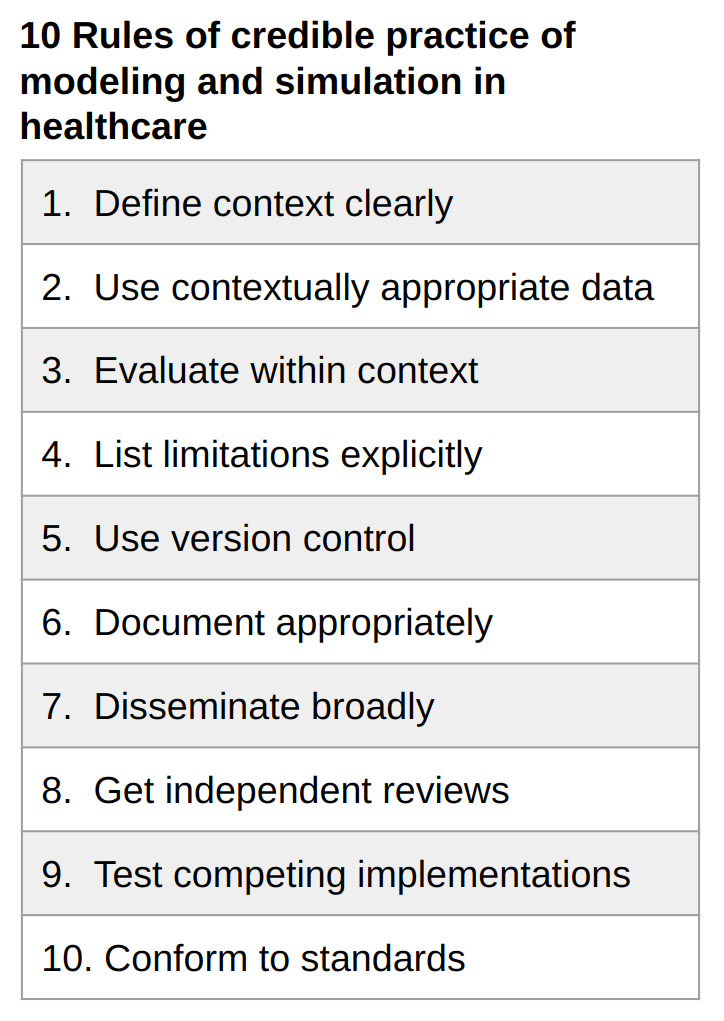
\includegraphics[width=6cm]{images/10rules.png}
    \captionof{figure}{The Committee on Credible Practice of Modeling and Simulation in Healthcare 10 rules of model credibility.}
    \label{fig:10rules}
\end{center}


\section{Qualitative Credibility Assessment in Other Modeling Fields}
NASA and the FDA also have a keen interest in producing well-documented and credible models for the purpose of making critical decisions. However, modeling and simulation tasks in these institutions are far broader compared to systems biology. NASA models range from the analysis of individual parts to orbits and spacecraft while models submitted to the FDA include medical devices and pharmacokinetics. Due to the wide variety of modeling tasks relevant to NASA and the FDA, credibility guidelines in these institutions are general, largely qualitative, and do not prescribe specific tests.


\subsection{NASA Credibility Assessment Scale}

After the loss of the Columbia Space Shuttle and its seven crew members in 2003, NASA significantly increased its focus on quantitative and credible models. The misuse of an existing model and the reliance on engineers' judgment led to the false conclusion that shuttle reentry would not be affected by a small hole in the heat shield caused by a debris strike during takeoff~\cite{Blattnig2013-qx, Howell2021}. The lack of quantifiable uncertainty and risk analysis in the report to management ultimately led to the shuttle's disintegration~\cite{Niewoehner2008}. Since then, NASA has developed extensive modeling and simulation standards including the Credibility Assessment Scale~\cite{babula_nasa_2009} (CAS) (figure \ref{fig:NASA}).  

Each model credibility standard described here emphasizes assessments be made within a specific context of use, the specific role and scope of the model and the specific question of interest that the model is intended to help answer~\cite{FDAguidelines}. The judgment error that ultimately led to the Columbia Space Shuttle disaster was partially due to the use of a modeling software far outside the intended context of use, leading to incorrect predictions and over-reliance on engineer's judgment~\cite{Blattnig2013-qx}. In addition to specifying the scope and question of interest, the context of us should also describe how model outputs will be used to answer the question of interest and whether other information, such as bench-testing, will be used in conjunction with the model to answer the question of interest~\cite{FDAguidelines}. The standards described here, from various institutions such as NASA and the FDA, all specify that credibility is to be evaluated within a specific context of use.

\begin{center}
    \captionsetup{type=figure}
    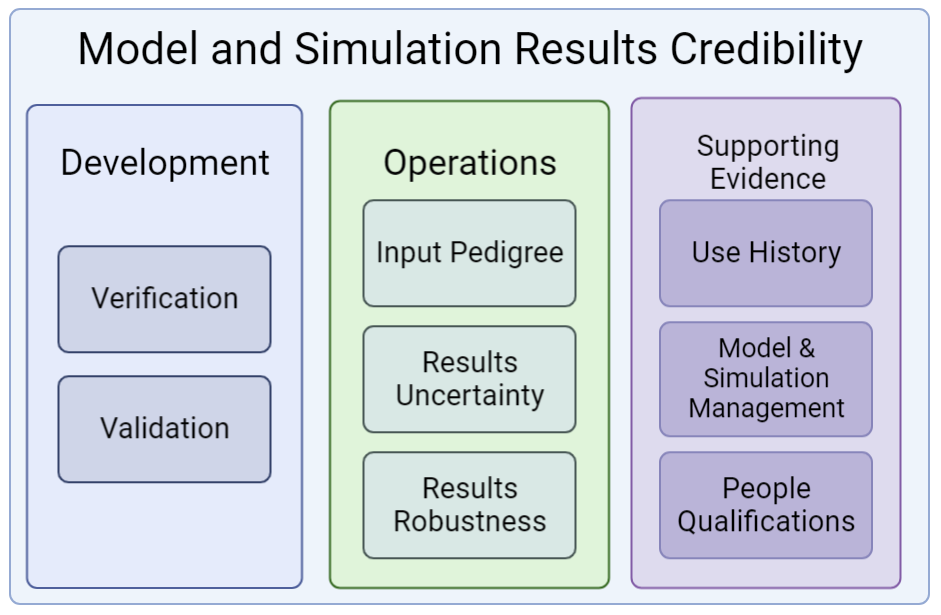
\includegraphics[width=8.5cm]{images/NASA_CAS.png}
    \captionof{figure}{Categories of the NASA Credibility Assessment Scale (CAS)}
    \label{fig:NASA}
\end{center}


NASA's CAS is intended to help a decision-maker evaluate the credibility of specific modeling and simulation results and to identify aspects of the results that most influence credibility~\cite{blattnig_towards_2008, Blattnig2013-qx}. The credibility assessment process can be viewed as a two part process: first the modeler conveys an assessment of the results, then a decision maker infers the credibility of these results. The CAS standard consists of eight factors grouped into three categories~\cite{babula_nasa_2009}: development, operations, and management. Each of the eight factors is scored on a scale of 0-4 with guidelines for each numeric score. These factors were selected as they were considered to be the most essential, sufficiently independent of one another, and could be objectively assessed. While the primary concern is the score for each individual factor, the secondary concern is the score of the overall model, which is the minimum score of the eight subfactors. 

The model and simulation (M\&S) development category consists of subsections verification and validation~\cite{babula_nasa_2009}. Scoring in these subcategories assess the correctness of the model implementation, the numerical error and uncertainty, and the extent to which the M\&S result matches reference data. If numerical errors for important features are ``small" and if results agree with real-world data, the highest score of 4 is awarded for these factors.

The second category, M\&S operations, consists of three factors: input pedigree, results uncertainty, and result robustness~\cite{babula_nasa_2009}. Input pedigree describes the level of trust in the input data, where input data that accurately reflects real-world data receiving the highest score. The results uncertainty category earns the highest score if non-deterministic numerical analysis is performed. Result robustness high scores are achieved by including sensitivity analysis for most parameters and identifying key sensitivities.

Model and simulation management, the third category, is less technical, containing the factors use history, M\&S management, and people qualification~\cite{babula_nasa_2009}. Use history scores the highest score if the model has previously been used successfully and meets de facto standards. For example, a model used for finite element analysis (FEA) would be required to meet FEA standards and codes for the type of object being modeled. M\&S management refers to the maintenance and improvement of the model with continual process improvement receiving the highest score of 4.  The people qualification category assesses the experience and qualifications of those constructing, maintaining, and using the model where personnel with extensive experience with the model and best practices scoring the highest. 

Although these categories were chosen, in part, due to their ability to be objectively assessed, there is still a significant subjective component of the scoring process. It is acknowledged that different decision makers may assign different degrees of credibility to the same model and different decisions may require different levels of credibility. The CAS serves as a template to assess and clearly communicate risks to decision-makers. Additionally, it can be useful in measuring model development progress or in identifying areas where improvement is most needed~\cite{Blattnig2013-qx}.


\subsection{Credibility Standards for Medical Models}
In addition to systems biology, computational models are also becoming essential tools in biomedical applications such as drug discovery~\cite{Chen2015}, pharmacokinetics~\cite{Kuh2000}, and medical devices~\cite{Kung2019}. Credibility is essential in biomedical modeling, particularly in cases where models influence patient treatment or regulatory approval of a device or drug. Both the FDA and the European Medicines Agency have developed standards guiding model credibility for the purposes of regulatory approval. As with NASA, these guidelines are broad and qualitative due to the broad scope of biomedical modeling. Before the FDA began formalizing guidelines for model credibility, the American Society of Mechanical Engineers (ASME) issued Verification and Validation (V\&V) 40 for assessing credibility of computational models in medical device applications~\cite{viceconti_credibility_2020}. However, this standard assumes the ability to perform traditional validation activities such as comparing model predictions to well-controlled validation experiments~\cite{FDAguidelines}, a task which can be unfeasible with some biomedical models. Many models used in regulatory submissions are supported by many sources of evidence beyond traditional validation experiments including clinical trials and population-level validation. Recognizing this fact, FDA modeling credibility guidelines expand on ASME V\&V 40 concepts to provide a more general framework for assessing a wider variety of models.


\subsubsection{ASME V\&V 40}

The ASME developed the V\&V 40 standard in 2012 as a means of describing verification and validation activities in the modeling and simulation of medical devices~\cite{viceconti_credibility_2020}. Like the NASA CAS, V\&V 40 focuses on context of use, model risk, and the establishment of credibility goals prior to any credibility assessment. The context of use addresses the specific role of the model in addressing the question of interest. Model risk is then assessed based on the possibility that the model may lead to incorrect conclusions resulting in adverse outcomes. After the establishment of credibility goals, verification and validation take place. 

Of particular relevance to modeling in systems biology are the descriptions of code and calculation verification found in V\&V 40. Verification seeks to determine if the model is built correctly. More specifically, code verification aims to identify any errors in the source code and numerical algorithms. This can be done by comparing output from a model to benchmark problems with known solutions~\cite{viceconti_credibility_2020}. Calculation verification estimates the error in the output of a model due to numerical methods. Output errors can include discretization errors, rounding errors, numerical solver errors, or user errors. Calculation verification is complete when it is demonstrated that errors in the numerical solution are minimized to the point that they are not corrupting the numerical results~\cite{viceconti_credibility_2020}.

Validation assesses how well the computational model represents reality. Validation activities might include comparing the model's behavior to the biological features of the real phenomenon by comparing results to \textit{in vitro/in vivo} benchmark experiments. Validation also includes uncertainty quantification and sensitivity analysis. Uncertainty quantification refers to the estimation of how stochastic error in the input propagates into the model's output. Sensitivity analysis is a post-hoc examination of the results of the uncertainty quantification to evaluate which elements most influence output variability~~\cite{viceconti_credibility_2020}.

Unlike the NASA CAS, V\&V 40 does not describe the quality of evidence needed to prove a model credible and lacks an objective scoring system necessary for implementing ``cut-offs" of credible versus non-credible models, or for comparing the credibility of multiple models.

\subsubsection{FDA Guidance on Computational Model Credibility in Medical Devices}

Based on the V\&V 40 standard, the FDA released guidance on assessing credibility for models of medical devices~\cite{FDAguidelines}. This guidance expands V\&V 40 to include other forms of credibility evidence beyond traditional verification and validation exercises. Applicable to physics-based, mechanistic, or other first-principles-based models of medical devices, these guidelines consist of ten categories broadly divided into code verification, calculation verification, and validation. The code verification category is taken directly from V\&V 40 described previously.

The calculation verification guideline extends the V\&V 40 by detailing several methods to verify that the model produces the intended output.  For example, the model results can be compared with the same data used to calibrate the model parameters. Broader evidence in support of the model, but perhaps without a specific context of use are also acceptable. A model can also be verified using \textit{in vitro} or \textit{in vivo} experiments either within the context of use, or within conditions supporting a different context of use. These techniques can also be used for validation evidence. 

Validation assesses the model's ability to reproduce real-world behavior. In addition to the methods described for calculation verification, validation can also include population-based evidence, statistical comparisons of model predictions to population-level data such as the results of a clinical trial. Credibility is also supported by emergent model behavior, the ability of a model to reproduce real-world phenomena that were not pre-specified or explicitly modeled, as well as general model plausibility, that model assumptions, input parameters, and other characteristics are deemed reasonable based on scientific knowledge of the system modeled. 

Unlike the NASA Credibility Assessment Scale, these FDA guidelines are sets of nonbinding recommendations. Additionally, no scoring or suggested quality measures of FDA credibility factors are included making quantitative analysis of credibility impossible.


\subsubsection{EMA Guidelines for PBPK Models}

Of particular relevance for the field of systems biology is The European Medicines Agency's (EMA) Guideline on the Reporting of Physiologically Based Pharmacokinetic (PBPK) Modeling and Simulation issued in 2018~\cite{viceconti2021, Shepard2015} . PBPK models are mathematical models that simulate the concentration of a drug over time in tissues and blood. With the rise in regulatory submissions that include PBPK models that rely on specialized software programs, this guideline provides detailed advice on what to include in a PBPK modeling report. 

The standard dictates the necessary information to describe and justify model parameters. Like the FDA standard, modelers are required to submit any assumptions made when assigning parameters and to document the sources of any literature-based parameters. Additionally, modelers must perform a sensitivity analysis for parameters that are key to the model (those that significantly influence the outcome) and list any parameters that are uncertain. 

The submission must include the simulation results as well as the files used to generate the final simulations in both tabular and executable format. This requirement is shared with reproducibility standards already in place for systems biology in the COMBINE Archive standard as well as described in systems biology modeling reproducibility best practices~\cite{porubsky_best_2020}.

The predictive performance of the model must also be evaluated. That is, its ability to recapitulate observed pharmacokinetics. This requirement is also mentioned in the FDA guidelines. 

Lastly, the guideline requires a discussion of uncertainty and confidence in the model. Although described more qualitatively in the EMA standard, this requirement is shared by NASA's CAS, V\&V 40, FDA credibility guidelines, and best practices for reproducible modeling in systems biology~\cite{porubsky_best_2020}.




\subsection{Current Tools for Systems Biology Model Testing}
Although there is no credibility standard in systems biology modeling, some tools provide automated model testing. Although these tools were not developed explicitly to assess credibility, many of the factors they test for could be considered aspects of credibility. Future model credibility assessments could aspire to the level of quantification and automation these tools offer. 
 
\subsubsection{MEMOTE}
MEMOTE (MEtabolic MOdel TEsts) is an open-source Python software that automatically tests and scores genome-scale metabolic models~\cite{Lieven2020-kj}. MEMOTE offers a web interface and command line interface where SBML files can be uploaded and analyzed, and ultimately scored. The tests check that a model is annotated according to the MIRIAM standard, that components are described using SBO terms, and that the model is properly constructed using the relevant SBML package, SBML-FBC~\cite{Lieven2020-kj, Olivier2018-tx}. Basic tests check for the presence of relevant components, charge information, and metabolite formulas. Biomass tests check that biomass precursors are produced and that the growth rate is non-zero. Stoichiometry tests test for inconsistency, erroneously produced energy metabolites, and reactions that are permanently blocked. A numeric score is output after testing indicating the extent to which a model conforms to these standards.

MEMOTE is designed to assess genome-scale metabolic models and largely includes tests that are specific to this model subset. Although a high MEMOTE score is likely to be indicative of model quality and reproducibility, it is not an assessment of credibility. A credible model will likely have a good MEMOTE score, but a good MEMOTE score does not necessarily indicate a credible model. However, the quantitative and automated nature of MEMOTE allows for quickly gauging model quality, comparing models, and the iterative improvement of metabolic models.

\subsubsection{FROG Analysis}
Similar to MEMOTE, the COMBINE community has recently developed FROG analysis, an ensemble of analyses for constraint-based models to generate standardized numerically reproducible reference datasets~\cite{sbmlsim21}. Results from constraint-based models are often communicated as flux values and there are often multiple solutions for a single model. As such, results cannot be used to gauge reproducibility. The COMBINE community outlined a list of outputs and results of flux balance analysis that are numerically reproducible and can be used for curation, known as FROG reports. FROG reports can be used in the BioModels~\cite{BioModels2018a, BioModels2020} curation process to assess reproducibility.

FROG analysis consists of  \textbf{F}lux variability analysis, \textbf{R}eaction deletion, \textbf{O}bjective function values, and \textbf{G}ene deletion fluxes. Flux variability analysis tests that the maximum and minimum fluxes are reproducible using different software tools. The objective function value for a defined set of bounds should be reproducible. The systematic deletion of all reactions or all genes, one at a time, should provide comparable reference results. Currently four tools support the generation of FROG reports. Web-based tools include fbc\_curation~\cite{sbmlsim21}, CBMPy MOdel Curator~\cite{SBMpy} (both of which are also available as command line tools), and FLUXER~\cite{hari2020}. fbc\_curation\_matlab is a command-line tool and exports results in COMBINE archive format~\cite{fbc_curation}.

Unlike MEMOTE, FROG analysis produces a report in lieu of a single numerical score. 

\section{Discussion}
When standards are established, tests can be established to assess the extent to which a model conforms to that standard. With the development of standardized quantitative metrics (as opposed to qualitative guidelines such as those discussed previously), models can be constructed to meet minimum quality requirements lending credibility to those models and allowing for easy comparison across models~\cite{Kaddi2007-js}. 

The difficulty in developing these quantitative metrics is that the characteristics of an ideal bio-model must be known and expressed concisely. Existing standards in systems biology seek to address the first point by outlining what information is necessary to completely define and reproduce a model as well as the format in which that information is to be presented. However, a model could meet all existing standards and not be credible. For example, a model could be fully defined in SBML with extensive annotations, be reproducible, properly formatted for dissemination with SED-ML files describing all simulations. Despite meeting these standards, this hypothetical model could produce negative concentrations when simulating, clearly indicating that the model is not credible.  Additional metrics and standards must be established to adequately assess credibility. These metrics might include the relative concentration of floating species or the shape of response curves.

Hellerstein \textit{et al.} note that several issues in biomedical modeling are analogous to problems faced in software development and propose that software development best practices might be translated to improve modeling in systems biology~\cite{Hellerstein2019}. Of particular interest is software testing, which can be considered a form of credibility assessment. These tests aim to ensure the correctness, reliability, and availability of software, all characteristics that are also essential in systems biology model credibility. 


Software tests can be divided into two categories, which may also be applicable in systems biology modeling: (i) black-box testing and (ii) white-box testing. Black-box software testing assesses the behavior of the code and does not deal with implementation. For systems biology model credibility assessment, black-box credibility indicators might be that the model accurately predicts observed data. White-box testing evaluates the internal workings of a software project or model. The absence of errors, such as undefined parameters, typos, or unused species, might serve as white-box credibility indicators.  



\section{Conclusion}

Although many reproducibility standards are in use to simplify assessing reproducibility, there are no standards and scoring systems for model credibility in systems biology. Unlike institutions such as NASA and the FDA, which deal with models spanning a broad scope of applications and scales, systems biology is focused on the modeling of cellular processes. This narrow scope, combined with the variety of standards already in use, makes systems biology models well-suited for a credibility standard.

A quantitative credibility scoring system would be particularly useful and enable comparing the credibility of different models and guide the development of more credible models. Credibility metrics could be published alongside models to indicate the trustworthiness of results and allow users to make informed decisions about reusing models.


Systems such as MEMOTE demonstrate that model standards and model quality indicators can be automatically quantitatively scored enabling iterative improvement during the development phase. More challenging is further developing standards to express characteristics, both quantitative and qualitative, that make a model credible. Current modeling standards in other scientific fields emphasize assessing credibility in the model's context of use. This poses a challenge for automating credibility assessment in systems biology modeling as more or less rigor may be required to achieve a sufficiently credible model depending on the intended use of the model. It may prove useful to develop a manual, semi-quantitative scoring systems, such as NASA's Credibility Assessment Scale prior to attempting to implement a fully quantitative and perhaps automated credibility scoring system for systems biology models.

\subsection*{Funding}
This work was supported by NIH Imaging and Bioengineering (NIBIB) award P41GM109824, and the National Science Foundation award 1933453. 




\chapter{Summary}
The primary goal of this research was to develop a novel algorithm for evolving mass-action networks, package the algorithm in a user-friendly software tool, and explore what aspects of the algorithm drove its success. This work was influenced by earlier work, described in chapter \ref{chap: cesium_paper}, which involved software to evolve oscillating mass-action networks. The software had a low success rate and poor computational performance. The software, ReactionNetworkEvolution.jl, described in chapter \ref{chap: ReactionNetworkEvolution.jl} addresses these issues and increases the success rate 10 fold. 

In chapter \ref{chap: ReactionNetworkEvolution.jl}, the novel evolutionary algorithm is probed to understand what aspect of it drive evolutionary success. Various parameters and slight algorithm adjustments were trialed and the rates of evolutionary success (trials that produced oscillators) were compared. It was found that speciation most effects the success rate by encouraging population diversity and protecting innovations. Elite selection was also essential for evolutionary success. Unlike previous works in other domains, crossover was found to be detrimental to the algorithm's success. Based on what was learned during these experiments, the algorithm was optimized resulting in an evolutionary success rate of 51.9\%.


\begin{appendices}	
\chapter{The ReactionNetworkEvolution.jl Software}

\section{Introduction}
The purpose of this chapter is to briefly describe the logistics of acquiring, using, and customizing the ReactionNetworkEvolution.jl software. It describes how to use the package to generate oscillators, match time series data, and fit parameters for a network with fixed topology. This documentation may become obsolete as the ReactionNetworkEvolution.jl is updated and improved. For the most recent documentation, see \url{https://github.com/ltatka/ReactionNetworkEvolution.jl.git}.

\section{Download and Quick Start}
ReactionNetworkEvolution.jl is currently available as a github repository or a julia package. The package requires the julia programming language, version 1.9.0, which can be downloaded with directions from the julia website, \url{https://julialang.org/downloads/ }. The package was designed to run on both linux and windows machines.

To use ReactionNetworkEvolution.jl as a script, it is best to clone the github repository in order to be certain of it's location.

In a terminal, clone the github repository, located at \url{https://github.com/ltatka/ReactionNetworkEvolution.jl.git} and navigate to the newly created ReactionNetworkEvolution.jl directory.


\begin{Verbatim}[frame=single]
	git clone https://github.com/ltatka/ReactionNetworkEvolution.jl.git
	cd ReactionNetworkEvolution.jl
\end{Verbatim}

In the ReactionNetworkEvolution.jl, there is a script titled, run\_evolution.jl. This script can be run from any terminal. Upon execution, the script will instantiate all dependencies. A JSON file containing all default settings, settings.json, is also available in the ReactionNetworkEvolution.jl directory. This file can be modified to adjust settings and will be automatically read by the run\_evolution.jl script. 

ReactionNetworkEvolution.jl supports several command line arguments for the most frequently changed settings. These include the number of trials, generations, and population size as well as paths to additional settings and an output directory and random seed (table \ref{table:flag_args}). For example, a user can change the number of generations on the command line as follows:


\begin{Verbatim}[frame=single]
	julia run_evolution.jl --ngenerations=1600
\end{Verbatim}



ReactionNetworkEvolution.jl can also be downloaded as a julia package. The advantages of this method is that ReactionNetworkEvolution.jl is accessible from any working directory. The disadvantage is that the package is installed in the julia packages directory. This directory can be difficult to locate making the run\_evolution.jl script less accessible.

When downloading ReactionNetworkEvolution.jl as a package, it can be imported and its functions used in a julia programming environment. The ``Pkg.add" command only needs to be performed once to download the package. After it is added to the local package repository, it can be called with ``using" or ``import."

\begin{Verbatim}[frame=single]
	julia # activate the julia interpreter
	using Pkg
	Pkg.add("ReactionNetworkEvolution") 
	
	# To run a trial of evolution using the default settings:
	import ReactionNetworkEvolution as rne
	rne.run_evolution()	
\end{Verbatim}

When using the run\_evolution \textit{function}, the command line arguments described previously can be supplied as optional keyword arguments. 


\begin{Verbatim}[frame=single]
	rne.run_evolution(ngenerations=1200)
\end{Verbatim}



By default, ReactionNetworkEvolution.jl prints its progress in the terminal as well as what settings directory and output directories are used. An example of the output is shown below. The compilation time and evolution time are also returned. Timing data omits any post-processing steps.


\begin{Verbatim}[frame=single]
Starting 2024-06-03 12:52:53
Writing output to /home/outputpath/evolution_output
Using default settings
Beginning 5 trials with 50 generations each
..... trial 5
 21.693363 seconds 
Output written to /home/evolution_output/batch_2024-06-03_125253sNA
Done
\end{Verbatim}

\begin{table}
    \centering
    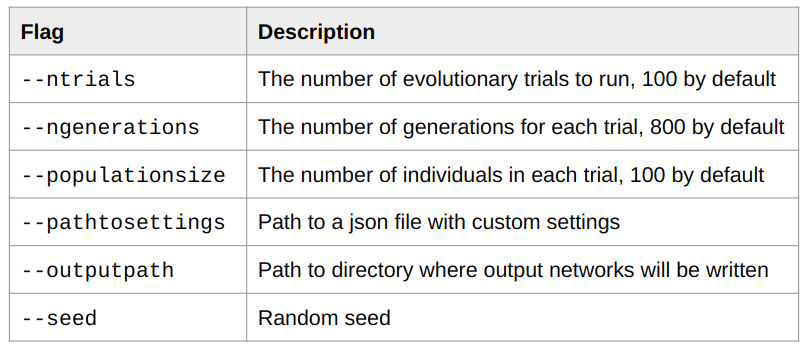
\includegraphics[width=15cm]{images/flag_args_table.png}
    \caption[Description of command line flag arguments]{Command line flag arguments. Flag arguments take precedence over customizations in a JSON file.}
    \label{table:flag_args}
\end{table}


\section{Further Customization}
Beyond the basic customizations available with command line arguments, there are many settings options that can be adjusted with a JSON file. The JSON file is written as a dictionary, with the name of the setting as the key. The user then supplies the path to the JSON settings file as a command line argument. Settings can be specified in any order. Any settings that are not specified will be set to the default value. All settings and their default values are described in table \ref{table:hyperparams}.

\begin{Verbatim}[frame=single]
	# Example customization file
	{"populationsize": 200,
	"p_crossover": 0.25,
	"ngenerations": 1600}
\end{Verbatim}

\begin{Verbatim}[frame=single]
# Supplying the custom settings JSON file
julia --project=. run_evolution.jl --pathtosettings="/path/settings.json"
\end{Verbatim}


\begin{table}

    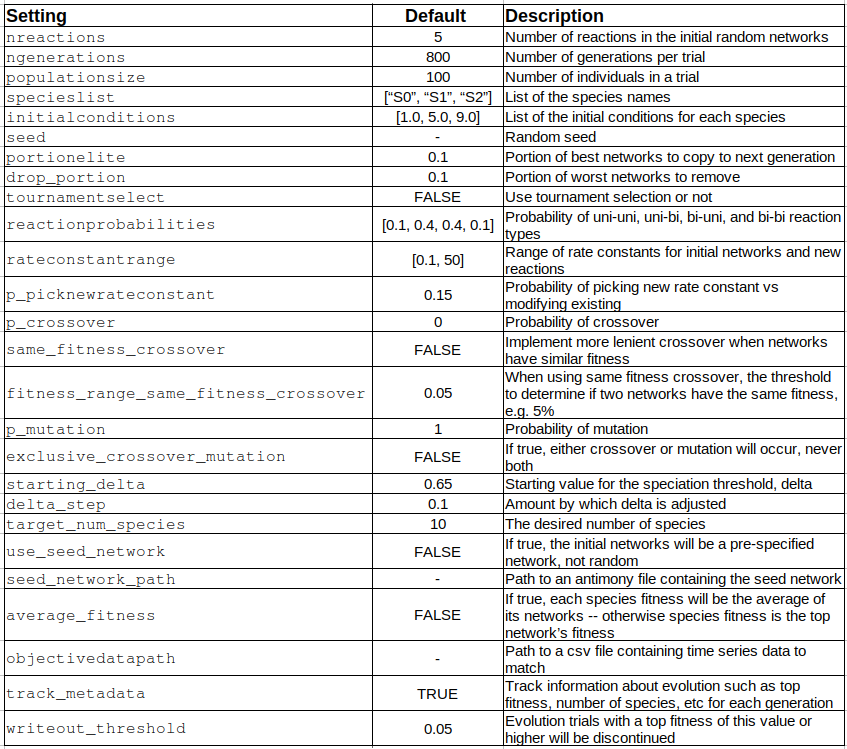
\includegraphics[width=18cm]{images/hyperparams.png}
    \caption[Evolution algorithm settings]{Evolutionary algorithm settings and default values.}
    \label{table:hyperparams}
\end{table}

\section{Fit Arbitrary Timeseries Data}
As described in section \ref{section:fit_timeseries}, ReactionNetworkEvolution.jl can be used to generate models to match input timeseries data. ReactionNetworkEvolution.jl can take any timeseries data in the form of a csv file with the leftmost column being time. Supply the path to the timeseries data to the ``objective\_data\_path" setting in a JSON file. Either modify the included settings.json file or create a new settings file and supply it with the ``pathtosettings" command line argument.

\section{Parameter Fitting}
ReactionNetworkEvolution.jl can also be used to fit parameters (rate constants) for a network with fixed topology. Supply the path to the antimony file containing the network to the ``seed\_network\_path" setting and specify ``use\_seed\_network" as true. To avoid modifying reactions, set ``p\_rateconstant\_mutation" to 1. In order to take advantage of speciation despite having a population of topologically identical networks, set ``rateconstant\_distance\_weight" to 1 or any positive nonzero number. Parameter fitting with fixed topology may be a case where crossover proves useful. It may help to set ``p\_crossover" to 0.25 or another positive number between 0 and 1. 

\begin{Verbatim}[frame=single]
	# Example json file for parameter fitting with fixed topology
	{"use_seed_network": true,
	"seed_network_path": "/path/seednetwork.ant",
	"p_rateconstant_mutation": 1,
	"rateconstant_distance_weight": 1}
\end{Verbatim}

\section{Post-Processing}
By default, ReactionNetworkEvolution.jl will write out all final models and a JSON file with the top fitness for each generation. For oscillators, final models can automatically be assessed by setting the ``process\_output" setting to true. When evolution is complete, each final model will be evaluated and network files and their associated fitness JSON files will be sorted into a directory labeled either ``SUCCESS" or ``FAIL." 

The package also includes a python package with some post-processing utilities. In some cases, it appears that the python functions more accurately sort oscillators and non-oscillators. 

To use the python utilities package, the working directory must be ReactionNetworkEvolution.jl. The location of this directory can be specified by downloading the package using git as opposed to the ``Pkg.add" function.

\begin{Verbatim}[frame=single]
	# To import the python utilities package
	import utilities as util
\end{Verbatim}

\subsection{Python Utilities Sub-Package}
The key functions in the python utilities ``sub-package" are described here.

\subsubsection{evaluate\_oscillators(path: str)}
Given a directory of antimony files, this function simulates each network and labels the file as ``success" if it is an oscillator, otherwise ``fail." This function appears to be more accurate than the julia equivalent function for reasons unknown. \\
\underline{Parameter} Path: (str) Path to a directory of antimony models\\
\underline{Returns} (int, int) The number of oscillators found and the total number of models evaluated

\subsubsection{evaluate\_fitness\_cutoff(path: str, cutoff: float)}
Similar to the evaluate\_oscillators function, this function sorts through a directory of antimony models and labels them ``success" if the fitness is above the input threshold, otherwise they are labeled ``fail." It seems that 0.01 is a good cutoff to distinguish between oscillators and non-oscillators with few false negatives or false positives. \\
\underline{Parameter} path: (str) Path to a directory of antimony models\\
\underline{Parameter} cutoff: (float) Fitness cutoff value (0.01 recommended)\\
\underline{Returns} (int, int) The number of oscillators found and the total number of models evaluated

\subsubsection{sort\_by\_fitness(path: str)}
Given a directory of antimony files, sort them by fitness (best to worst) and relabel the files accordingly.\\
\underline{Parameter} path: (str) Path to a directory of antimony models\\
\underline{Returns} None

\subsubsection{plot\_timeseries(input, start=0, end=1, numpoints=200, savepath=None)}
Plot the timeseries data for either a single or multiple network models. If multiple, plots will appear as an array of subplots.\\
\underline{Parameter} input: any of
\begin{itemize}
\item{(str) path to a directory containing antimony files}
\item{list(str) or list(RoadRunner): a list of antimony strings or RoadRunner} models
\item{(str) or (RoadRunner): a single antimony string or RoadRunner model}
\end{itemize}
\underline{Optional Parameters}
\begin{itemize}
\item{start (float): start time for simulation}
\item{end (float): end time for simulation}
\item{numpoints (int): the number of time points for simulation}
\item{savepath (str): path to save the plot}
\end{itemize}
\underline{Returns} None


\subsubsection{plot\_fitness(path: str, limit: int=None, savepath: str=None)}
Plot the top fitness value for each generation for each network model\\
\underline{Parameter} input (str) path to directory containing JSON files of fitness values\\
\underline{Optional Parameters}
\begin{itemize}
\item{limit (int): the maximum number of fitness trajectories to plot}
\item{savepath (str): path to save the plot}
\end{itemize}
\underline{Returns} None

\subsubsection{prune\_models(path: str)}
Many models contain extraneous reactions that are not necessary for reaction. This function takes a directory of antimony files and evaluates each network model to remove any extra reactions by commenting them out. \\
\underline{Parameter} path: (str) Path to a directory of antimony models\\
\underline{Returns} (int, int): the total number of reactions removed and the total number of models evaluated


\end{appendices}	

% Bibliography
\bibliographystyle{plain}
\bibliography{researchbib}
\end{document}


